\documentclass[
  % journal=largetwo,
  journal=pasa,
  manuscript=article-type,
  year=2020,
  volume=37,
]{cup-journal}

\usepackage{amsmath}
\usepackage[nopatch]{microtype}
\usepackage{booktabs}
\usepackage{mathtools}
\usepackage{amssymb}
\usepackage[caption=false]{subfig}
\usepackage{tabularx}
\usepackage{multirow}

\newcommand{\vdag}{(v)^\dagger}
\DeclareMathAlphabet\mathbfcal{OMS}{cmsy}{b}{n}
\DeclareMathOperator{\vect}{vec}

\title{Comparison of Fast Imaging Architectures for Large, Multi-scale, Hierarchical Aperture Arrays}

\author{Nithyanandan Thyagarajan}
\affiliation{CSIRO, Space \& Astronomy, P. O. Box 1130, Bentley, WA 6102, Australia}
\email[Nithyanandan Thyagarajan]{Nithyanandan.Thyagarajan@csiro.au}

% \author{S. Author}
% \affiliation{Second Division, Organization, City, Pincode, State, Country}
% % \alsoaffiliation{Joint first authors}

% \author{T. Author}
% \affiliation{Second Division, Organization, City, Pincode, State, Country}

% \author{F.T. Author}
% \affiliation{Fourth Division, Organization, City, Pincode, State, Country}

% \addbibresource{example.bib}

\keywords{keyword entry 1, keyword entry 2, keyword entry 3} %% First letter not capped

\begin{document}

\begin{abstract}

\end{abstract}

\section{Introduction}

\cite{TMS2017}
\cite{Otobe+1994,Tegmark+2009,Tegmark+2010,Zheng+2014}
\cite{Morales2011,Thyagarajan+2017}
\cite{Cornwell+2008}
\cite{Beardsley+2017}

\section{Mathematical Notation}

Let $\mathcal{E}^\alpha_\nu(\hat{\boldsymbol{s}},t)$ represent the spectral Fourier components of the electric field time series emanating from astrophysical sources of emission in directions denoted by the unit vector, $\hat{\boldsymbol{s}}$, where, $\alpha\in\{1,2\}$ denotes the index of the polarisation state of the radiation, $\nu$ denotes the spectral component or the frequency of radiation, $\lambda=c/\nu$ is the wavelength, and $c$ is the speed of light. Hereafter, without loss of generality, all quantities can be implicitly assumed to depend on time and frequency throughout without explicit specification. Thus, $\mathcal{E}^\alpha(\hat{\boldsymbol{s}})\equiv \mathcal{E}^\alpha_\nu(\hat{\boldsymbol{s}},t)$

Electric fields in the aperture plane, $E^\alpha(\boldsymbol{r})$, can be written as a superposition of those that propagated from the astrophysical sources on the celestial surface $\mathbb{S}$:
\begin{align}
    E^\alpha(\boldsymbol{r}) &= \int_\mathbb{S} \mathcal{E}^\alpha(\hat{\boldsymbol{s}})\, e^{-i \frac{2\pi}{\lambda}\hat{\boldsymbol{s}}\cdot\boldsymbol{r}} \,\mathrm{d}\Omega,
\end{align}
where, the integral is over the celestial surface, $\mathbb{S}$, covered by the unit vector, $\hat{\boldsymbol{s}}$, $\boldsymbol{r}$ denotes the observer's location, $\mathrm{d}\Omega=\mathrm{d}^2\hat{\boldsymbol{s}}$ is the infinitesimal solid angle element on $\mathbb{S}$ perpendicular to $\hat{\boldsymbol{s}}$. 

The measuring instrument will imprint its transfer function on the measurements. If $a$ denotes a collecting element at location $\boldsymbol{r}_{a}$, then the electric field measured by this element will be
\begin{align}
    E_{a}^p &= \int_\mathbb{S} \sum_\alpha  \mathcal{W}_{a}^{p\alpha}(\hat{\boldsymbol{s}})\, \mathcal{E}^\alpha(\hat{\boldsymbol{s}})\, e^{-i \frac{2\pi}{\lambda} \hat{\boldsymbol{s}}\cdot\boldsymbol{r}_{a}} \,\mathrm{d}\Omega + n_{a}^p \, , \label{eqn:polarimetric-Efield-element-ideal}
\end{align}
where, $n_{a}^p$ and $\mathcal{W}_{a}^{p\alpha}(\hat{\boldsymbol{s}})$ are the stochastic noise and polarisation-sensitive directional electric field response of the element, $a$, respectively. $\mathcal{W}_{a}^{p\alpha}(\hat{\boldsymbol{s}})$ denotes the contribution from polarisation state, $\alpha$, in $\mathbb{S}$ to polarisation state, $p$, in the measurement.

Thus, the measured electric field can be treated as a linear superposition of the electric fields emanating from astronomical sources with appropriate complex phases acquired on account of propagation and properties of the measuring instrument. Ignoring wide-field effects, this relation can be simplified as a two-dimensional Fourier transform of the electric fields in the sky coordinates \cite{TMS2017}. Using the convolution theorem of Fourier transform, Equation~(\ref{eqn:polarimetric-Efield-element-ideal}) can be expressed as the weighted integral of the propagated electric field over the region the element is responsive to in the aperture surface, $\mathbb{R}$, 
\begin{align}
    E_{a}^p &= \int_\mathbb{R} W_{a}^{p\alpha}(\boldsymbol{r}_{a} - \boldsymbol{r})\,E^\alpha(\boldsymbol{r}) \, \mathrm{d}^2 \boldsymbol{r}+ n_{a}^p \, , \label{eqn:polarimetric-Efield-element-ideal-aperture-continuous}
\end{align}
where, the weighting, denoted by $W_{a}^{p\alpha}(\boldsymbol{r})$, is the spatial Fourier transform of $\mathcal{W}_{a}^{p\alpha}(\hat{\boldsymbol{s}})$,
\begin{align}
    W_{a}^{p\alpha}(\boldsymbol{r}) &= \frac{1}{\lambda^2}\int_\mathbb{S} \mathcal{W}_{a}^{p\alpha}(\hat{\boldsymbol{s}})\, e^{-i\frac{2\pi}{\lambda} \hat{\boldsymbol{s}}\cdot \boldsymbol{r}} \,\mathrm{d}\Omega \, . \label{eqn:holographic-Efield-illumination}
\end{align}

Equation~(\ref{eqn:polarimetric-Efield-element-ideal-aperture-continuous}) involves a weighted integral of the propagated electric fields, where the weighting corresponds to the instrumental response, $W_{a}^{p\alpha}(\boldsymbol{r})$, centered at the location of the element, $a$, in the aperture plane, $\mathbb{R}$. Generally, $W_{a}^{p\alpha}(\boldsymbol{r})$ is physically interpretable as the holographic pattern of the element element in the aperture plane, which has support over the element's area of influence where it collects signals from. 
% However, in some cases such as for narrow dipoles, this relation is purely mathematical and a physical interpretation is not straightforward. 
% such as narrow dipoles, this relation is  encapsulates the aperture field illumination pattern of the element or the element's aperture distribution, 
$W_{a_m}^{p\alpha}(\boldsymbol{r})$ can also include other instrumental effects that influence the element behavior. 

Equations~(\ref{eqn:polarimetric-Efield-element-ideal}) and (\ref{eqn:polarimetric-Efield-element-ideal-aperture-continuous}) can be discretised as:
\begin{align}
    E_{a}^p &= \sum_k e^{-i\frac{2\pi}{\lambda}\hat{\boldsymbol{s}}_k\cdot\boldsymbol{r}_{a}} \, \sum_\alpha \left[\mathcal{W}_{a}^{p\alpha}(\hat{\boldsymbol{s}}_k) \, \mathcal{E}^\alpha(\hat{\boldsymbol{s}}_k)\right] \, \delta\Omega_k + n_{a}^p \, , \label{eqn:Efield-element-img-discrete}
\end{align}
and
\begin{align}
    E_{a}^p &= \sum_j \sum_\alpha W_{a}^{p\alpha}(\boldsymbol{r}_{a}-\boldsymbol{r}_j)\, \delta^2\boldsymbol{r}_j \left(\sum_k e^{-i\frac{2\pi}{\lambda} \hat{\boldsymbol{s}}_k\cdot\boldsymbol{r}_j} \, \mathcal{E}^\alpha(\hat{\boldsymbol{s}}_k) \,\delta\Omega_k \right) \nonumber\\ 
    &\quad + n_{a}^p \, , \label{eqn:Efield-element-aperture-discrete}    
\end{align}
respectively. Equation~(\ref{eqn:Efield-element-aperture-discrete}) can be represented linear algebraically as
\begin{align}
    \mathbf{E}_{[p,\boldsymbol{r}_{a}]} &= \mathbf{W}_{[p,\boldsymbol{r}_{a}\leftarrow \alpha,\boldsymbol{r}]} \, \mathbf{F}_{[\boldsymbol{r}\leftarrow \hat{\boldsymbol{s}}]} \, \boldsymbol{\mathcal{E}}_{[\alpha,\hat{\boldsymbol{s}}]} + \mathbf{n}_{[p,\boldsymbol{r}_{a}]} \, .
\end{align}
The subscripted variables on either side of $\leftarrow$ indicate the transformation carried out by the associated matrix. For example, $\mathbf{F}_{[\boldsymbol{r}\leftarrow \hat{\boldsymbol{s}}]}\coloneqq e^{-i\frac{2\pi}{\lambda} \hat{\boldsymbol{s}}_k\cdot\boldsymbol{r}_j}$ denotes the Fourier matrix transforming variables defined on sky grid, $\hat{\boldsymbol{s}}_k$, to the aperture grid, $\boldsymbol{r}_j$. And, $\mathbf{W}_{[p,\boldsymbol{r}_{a}\leftarrow \alpha,\boldsymbol{r}]}\coloneqq \{W_{a}^{p\alpha}(\boldsymbol{r}_{a}-\boldsymbol{r}_j)\}$ is a matrix, where each row corresponds to the holographic pattern of an element, $W_{a}^{p\alpha}(\boldsymbol{r}_j)$, and the columns correspond to the aperture grid locations, $\boldsymbol{r}_j$. In each row, the holographic weights are shifted to the element location, $\boldsymbol{r}_{a}$. 

The theory of mutual coherence has established the relation between the intensity distribution of spatially incoherent quasi-monochromatic emission, $I^{\alpha\beta}(\hat{\boldsymbol{s}})\coloneqq \bigl\langle \mathcal{E}^\alpha(\hat{\boldsymbol{s}}) \mathcal{E}^{\beta *}(\hat{\boldsymbol{s}}) \bigr\rangle$ on $\mathbb{S}$ and mutual coherence, or visibility, $V^{\alpha\beta}(\Delta\boldsymbol{r})\coloneqq \bigl\langle E^\alpha(\boldsymbol{r})E^{\beta *}(\boldsymbol{r}+\Delta\boldsymbol{r})\bigr\rangle$, in the aperture plane, and is popularly known as the \textit{Van Cittert-Zernike} theorem \citep{VanCittert1934,Zernike1938,Born-Wolf,Goodman2000,TMS2017}:
\begin{align}
    V^{\alpha\beta}(\Delta\boldsymbol{r}) &= \int_\mathbb{S} \mathcal{I}^{\alpha\beta}(\hat{\boldsymbol{s}})\, e^{-i\frac{2\pi}{\lambda} \hat{\boldsymbol{s}}\cdot\Delta\boldsymbol{r}} \,\mathrm{d}\Omega, \label{eqn:VCZ-theorem}
\end{align}
where, $\Delta\boldsymbol{r}$, denotes the displacement vector between any two locations\footnote{The dependence of spatial coherence on $\Delta\mathbb{R}$ (displacement vectors between the element pairs), rather than $\mathbb{R}$ (absolute positions), in Equation~(\ref{eqn:VCZ-theorem}) implies an assumption of wide-sense spatial stationarity for the electric fields measured on the aperture, which will hold true only when the spatial intensity distribution, $\mathcal{I}^{\alpha\beta}(\hat{\boldsymbol{s}})$, on $\mathbb{S}$ is spatially incoherent.} in the aperture domain $\mathbb{R}$, $\langle\cdot\rangle$ denotes an estimator of the ensemble average\footnote{This is typically obtained by assuming ergodicity and averaging over a coherence scale usually along temporal or spectral axes, and sometimes over redundant element spacings.}, and $*$ denotes complex conjugation. When the instrument's transfer function is included in the measurement process, the visibility measured by the interferometer elements $a$ and $b$ (with separation $\Delta\boldsymbol{r}_{ab}\coloneqq \boldsymbol{r}_{a}-\boldsymbol{r}_{b}$) will be:
\begin{align}
    V_{ab}^{pq} &= \int_\mathbb{S} \sum_{\alpha,\beta} \mathcal{B}_{ab}^{pq;\alpha\beta}(\hat{\boldsymbol{s}})\,\mathcal{I}^{\alpha\beta}(\hat{\boldsymbol{s}})\, e^{-i\frac{2\pi}{\lambda} \hat{\boldsymbol{s}}\cdot\Delta\boldsymbol{r}_{ab}} \,\mathrm{d}\Omega + n_{ab}^{pq} \, , \label{eqn:ideal-polarimetric-visibilities}
\end{align}
where, 
\begin{align}
    \mathcal{B}_{ab}^{pq;\alpha\beta}(\hat{\boldsymbol{s}}) &=  \mathcal{W}_{a}^{p\alpha}(\hat{\boldsymbol{s}}) \mathcal{W}_{b}^{{q\beta }^*}(\hat{\boldsymbol{s}}) \, ,
\end{align}
is the directional polarimetric cross-power pattern of an ideal two-element interferometer (made of elements $a$ and $b$) measuring two polarizations, $p$ and $q$. Equation~(\ref{eqn:ideal-polarimetric-visibilities}) is the polarimetric radio interferometric measurement equation (RIME).  
% In the absence of other non-ideal effects, $\mathcal{B}_{a_m b_m}(\hat{\boldsymbol{s}})$ corresponds to the directional cross-power pattern of the interferometer comprising of elements $a$ and $b$.

From the Fourier transform relations, the above equations can be expressed equivalently in the aperture plane. The cross-power illumination of the interferometer's aperture, $B_{ab}^{pq;\alpha\beta}(\Delta\boldsymbol{r})$, is the Fourier transform of the directional cross-power pattern, $\mathcal{B}_{ab}^{pq;\alpha\beta}(\hat{\boldsymbol{s}})$,
\begin{align}
    B_{ab}^{pq;\alpha\beta}(\Delta\boldsymbol{r}) &= \frac{1}{\lambda^2}\int_\mathbb{S} \mathcal{B}_{ab}^{pq;\alpha\beta}(\hat{\boldsymbol{s}}) \, e^{-i\frac{2\pi}{\lambda} \hat{\boldsymbol{s}}\cdot \Delta\boldsymbol{r}_{ab}} \,\mathrm{d}\Omega \label{eqn:holographic-power-illumination} \\
    &= \int_\mathbb{R} W_{a}^{p\alpha}(\boldsymbol{r}) \, W_{b}^{q\beta *}(\boldsymbol{r}+\Delta\boldsymbol{r})\,\mathrm{d}^2\boldsymbol{r} \, ,
\end{align}
% In the aperture (Fourier) domain, it is equivalent to
% \begin{align}
%     B_{a_m b_m}^{pq;\alpha\beta}(\Delta\boldsymbol{r}) &= \int_\mathbb{R} W_{a_m}(\boldsymbol{r}) W_{b_m}^{*}(\boldsymbol{r}+\Delta\boldsymbol{r})\,\mathrm{d}^2\boldsymbol{r} \, ,
% \end{align}
which is a correlation of the aperture-plane responses of the two individual elements of the interferometer. The RIME in Equation~(\ref{eqn:ideal-polarimetric-visibilities}) can be expressed alternatively in the aperture domain as:
\begin{align}
    V_{ab}^{pq} &= \bigl\langle E_{a}^p \, E_{b}^{q*}\bigr\rangle\\ 
    &= \int_{\Delta\mathbb{R}} \sum_{\alpha,\beta} B_{ab}^{pq;\alpha\beta}(\Delta\boldsymbol{r}_{ab}-\Delta\boldsymbol{r})\,V^{\alpha\beta}(\Delta\boldsymbol{r})\,\mathrm{d}^2\Delta\boldsymbol{r}  + n_{ab}^{pq} \, , \label{eqn:vis-degridding}
\end{align}
whose discrete linear algebraic representation is
\begin{align}
    \mathbf{V}_{[pq,\Delta\boldsymbol{r}_{ab}]} &= \mathbf{B}_{[pq,\Delta\boldsymbol{r}_{ab}\leftarrow \alpha\beta,\Delta\boldsymbol{r}]} \, \mathbf{F}_{[\Delta\boldsymbol{r}\leftarrow \hat{\boldsymbol{s}}]} \, \boldsymbol{\mathcal{I}}_{[\alpha\beta,\hat{\boldsymbol{s}}]} + \mathbf{n}_{[pq,\Delta\boldsymbol{r}_{ab}]} \, .
\end{align}
Equation~(\ref{eqn:vis-degridding}) represents a weighting of the true spatial coherence of the incident radiation by the interferometer's cross-power illumination pattern and integration over the region the interferometer has a response to, centered at $\Delta\boldsymbol{r}_{ab}$. $\Delta\mathbb{R}$ denotes the space of all possible displacement vectors between elements. 

\section{Cost Metric} \label{sec:computational-cost}

The primary metric for computational cost used in this study is the number of real floating point operations (FLOP) and the rate of such operations measured in FLOPs per second (FLOPS). A complex addition consists of two FLOPs, and a complex multiplication consists of four real multiplications and two real additions and therefore six FLOPs. A complex multiply-accumulate (CMAC) operation includes one complex multiplication and addition, therefore requiring eight FLOPs.

Although alternate computational metrics that include additional components, such as memory bandwidth, could be justified from a practical standpoint, these metrics will vary significantly with real-life implementations and hardware components available. Therefore, we take a theoretical approach with the justification that the budget of floating point operations will form a lower bound regardless of the details of any particular implementation. 

\section{Multi-scale, Hierarchical Aperture Arrays} \label{sec:multi-scale-arrays}

We consider aperture arrays that operate interferometrically and hierarchically on multiple spatial scales. Examples of these multi-scale hierarchical aperture arrays include the Murchison Widefield Array \cite[MWA;][]{Tingay+2013}, the Low Frequency Array \cite[LOFAR;][]{vanHaarlem+2013}, the swarm of Long Wavelength Arrays \cite[LWA Swarm;][]{Dowell+2018}, and the Square Kilometre Array low \cite[SKA-low;][]{Dewdney+2009}. The specific spatial scales are the dimensions of the antenna, station (a grouping of antennas), and the array (a grouping of stations), denoted by $D_\textrm{a}$, $D_\textrm{s}$, and $D_\textrm{A}$, respectively. The number of stations in the array and the number of antennas in a station (indexed by $m$) are denoted by $N_\textrm{s}$ and $N_{\textrm{a/s}_m}$, respectively. 
% Although $N_\textrm{a/s_m}$ could vary with each station, we assume it remains the same for each station for simplicity. 

The specific aperture array examples we consider are the \texttt{SKA-low}, core of the SKA-low (\texttt{SKA-low-core}), low frequency Australian Very Long Baseline Array (\texttt{Aus-VLBA-low}), and low frequency inter-continental VLBA (\texttt{IC-VLBA-low}). The last two are hypothetical interferometers. It is assumed that $N_{\textrm{a/s}_m}=N_\textrm{a/s}=256$ (same for each station), $D_\textrm{a}/\lambda=1$, and $D_\textrm{s}/\lambda=17.5$ for each of these arrays, where, the nominal wavelength chosen here is $\lambda=2$~m. The corresponding station filling factor, $f_\textrm{s}=N_\textrm{a/s}\,(D_\textrm{a}/D_\textrm{s})^2$, is 0.836 for all the arrays. ~\texttt{SKA-low-core}, ~\texttt{SKA-low}, ~\texttt{Aus-VLBA-low}, and ~\texttt{IC-VLBA-low} are taken to consist of $N_\textrm{s}=256, 512, 512,$ and 512 stations in an array diameter of $D_\textrm{A}/\lambda=525, 3.25\times 10^4, 1.95\times 10^6$, and $3.9\times 10^6$, respectively. The corresponding array filling factors, defined as $f_\textrm{A}=N_\textrm{s}\,(D_\textrm{s}/D_\textrm{A})^2$, are 0.284, $1.48\times 10^{-4}$, $4.12\times 10^{-8}$, and $1.03\times 10^{-8}$, respectively. These parameters for the chosen examples are summarised in Table~\ref{tab:array_params}. 

% \begin{figure}
% \includegraphics[width=\linewidth]
% {figures/multidim_parameter_space.pdf}
% \caption{
% \label{fig:multidim-parameter-space}}
% \end{figure}

% \begin{table*}[htb!]
% \normalsize
% \begin{threeparttable}
% \caption{Table of multi-scale interferometer array parameters}
% \label{tab:array_params}
% \begin{tabular}{cccccccc}
% \toprule
% \headrow Array name & $D_\textrm{A}/\lambda$ & $N_\textrm{s}$ & $D_\textrm{s}/\lambda$ & $N_\textrm{a/s}$ & $D_\textrm{a}/\lambda$ & $f_\textrm{A}$\tnote{a} & $f_\textrm{s}$\tnote{b} \\
% \midrule
% \texttt{SKA-low-core} & $5.25\times 10^{2}$ & 256 & 17.5 & 256 & 1 & 0.284 & 0.836 \\ 
% \texttt{SKA-low} & $3.25\times 10^{4}$ & 512 & 17.5 & 256 &1 & $1.48\times 10^{-4}$ & 0.836 \\ 
% \texttt{Aus-VLBA-low} & $1.95\times 10^{6}$ & 512 & 17.5 & 256 & 1 & $4.12\times 10^{-8}$ & 0.836 \\
% \texttt{IC-VLBA-low} & $3.9\times 10^{6}$ & 512 & 17.5 & 256 & 1 & $1.03\times 10^{-8}$ & 0.836 \\ 
% % \midrule
% % Three & Four&three three\tnote{b} &four & & \\
% \bottomrule
% \end{tabular}
% \begin{tablenotes}[hang]
% % \item[]Table note
% \item[a]Array filling factor, $\,f_\textrm{A}=N_\textrm{s}\,(D_\textrm{s}/D_\textrm{A})^2$
% \item[b]Station filling factor, $\,f_\textrm{s}=N_\textrm{a/s}\,(D_\textrm{a}/D_\textrm{s})^2$
% \end{tablenotes}
% \end{threeparttable}
% \end{table*}

\begin{table*}[htb!]
\normalsize
\begin{threeparttable}
\caption{Table of multi-scale interferometer array parameters.}
\label{tab:array_params}
\begin{tabular}{cccccc|cc}
\toprule
\headrow Array name & $D_\textrm{A}/\lambda$ & $N_\textrm{s}$ & $D_\textrm{s}/\lambda$ & $N_\textrm{a/s}$ & $D_\textrm{a}/\lambda$ & $f_\textrm{A}$\tnote{a} & $f_\textrm{s}$\tnote{b} \\
\midrule
\texttt{LAMBDA-I} & $3.9\times 10^6$ & 4 & 17.5 & 256 & 1 & $1.61\times 10^{-10}$ & 0.836 \\ 
\texttt{SKA-low-core} & $5.25\times 10^{2}$ & 256 & 17.5 & 256 & 1 & 0.284 & 0.836 \\ 
\texttt{SKA-low} & $3.5\times 10^4$ & 512 & 17.5 & 256 & 1 & $1.28\times 10^{-4}$ & 0.836 \\ 
\texttt{CASPA} & $4.6\times 10^4$ & 3 & 8.08 & 65 & 0.5 & $9.2\times 10^{-8}$ & 0.996 \\ 
\texttt{FarView} & $6.77\times 10^2$ & 81 & 38.5 & 625 & 1 & 0.262 & 0.422 \\ 
% \texttt{LAMBDA-II} & $1.95\times 10^6$ & 32 & 17.5 & 256 & 1 & $2.58\times 10^{-9}$ & 0.836 \\ 
% \texttt{Aus-VLBA-low} & $1.95\times 10^{6}$ & 512 & 17.5 & 256 & 1 & $4.12\times 10^{-8}$ & 0.836 \\
% \texttt{IC-VLBA-low} & $3.9\times 10^{6}$ & 512 & 17.5 & 256 & 1 & $1.03\times 10^{-8}$ & 0.836 \\ 
% \midrule
% Three & Four&three three\tnote{b} &four & & \\
\bottomrule
\end{tabular}
\begin{tablenotes}[hang]
% \item[]Table note
\item[a]Array filling factor, $\,f_\textrm{A}=N_\textrm{s}\,(D_\textrm{s}/D_\textrm{A})^2$
\item[b]Station filling factor, $\,f_\textrm{s}=N_\textrm{a/s}\,(D_\textrm{a}/D_\textrm{s})^2$
\end{tablenotes}
\end{threeparttable}
\end{table*}

We have considered aperture arrays consisting of three spatial scales, but the analysis can be easily extended to other arrays consisting of even larger levels of spatial hierarchy. 

\section{Fast Imaging Architectures} \label{sec:img-archs}

We consider two broad classes of two-stage fast imaging architectures. In either case, the first stage is intra-station interferometry of the element electric fields using the options of voltage beamforming (BF), E-field Parallel Imaging Correlator (EPIC), beamforming of correlations (XBF), or correlation followed by FFT (XFFT). The second stage inter-station combination of the data products from the first stage. The main difference between the two classes is in whether the second stage uses the first stage products coherently or incoherently. A schematic of these hybrid architectures and their computational cost components are illustrated in Figure~\ref{fig:hybrid-architectures-cost-schematic}. Below, we provide details on the computational cost budget for these hybrid architectures along with the merits and demerits of either classes. 

Fast imaging involves processing data on multiple time scales. The channelisation of a voltage time stream of length $\delta t$ with a time resolution of $t_\textrm{s}$ will correspond to spectral channels of width $\delta\nu=1/\delta t$ and a bandwidth of $B=1/t_\textrm{s}$. The number of spectral channels is $N_\nu=B/\delta\nu=\delta t/t_\textrm{s}$. Images are expected to be produced at a cadence of $\Delta t$, which is typically larger than $\delta t$ and smaller than the time scale on which calibration needs to be updated. In this paper, the nominal values chosen for $\delta t$ is 25~$\mu$s, and we explore the possibilities for $\Delta t$ ranging from 0.1~ms to 10~s.  

\begin{figure*}
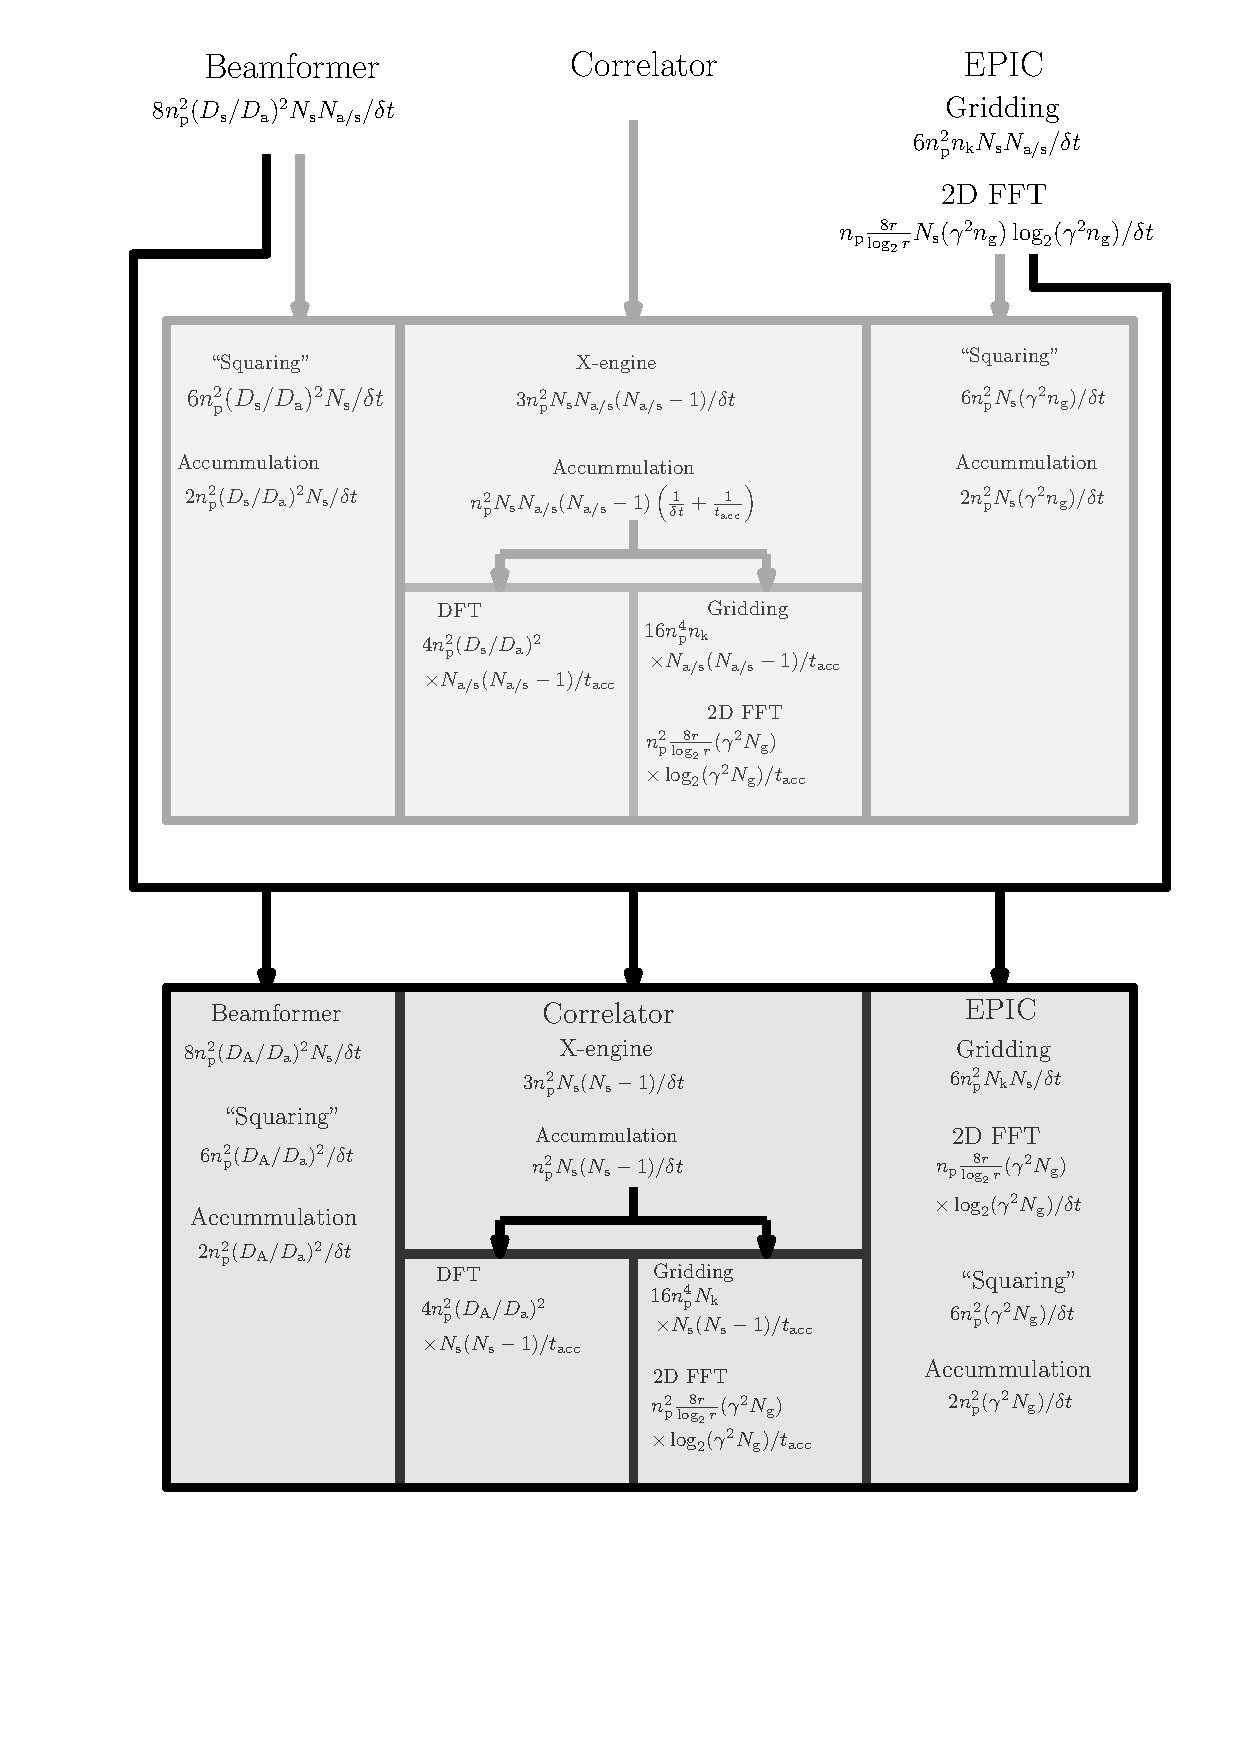
\includegraphics[width=\linewidth]{figures/flops_calc.pdf}
% 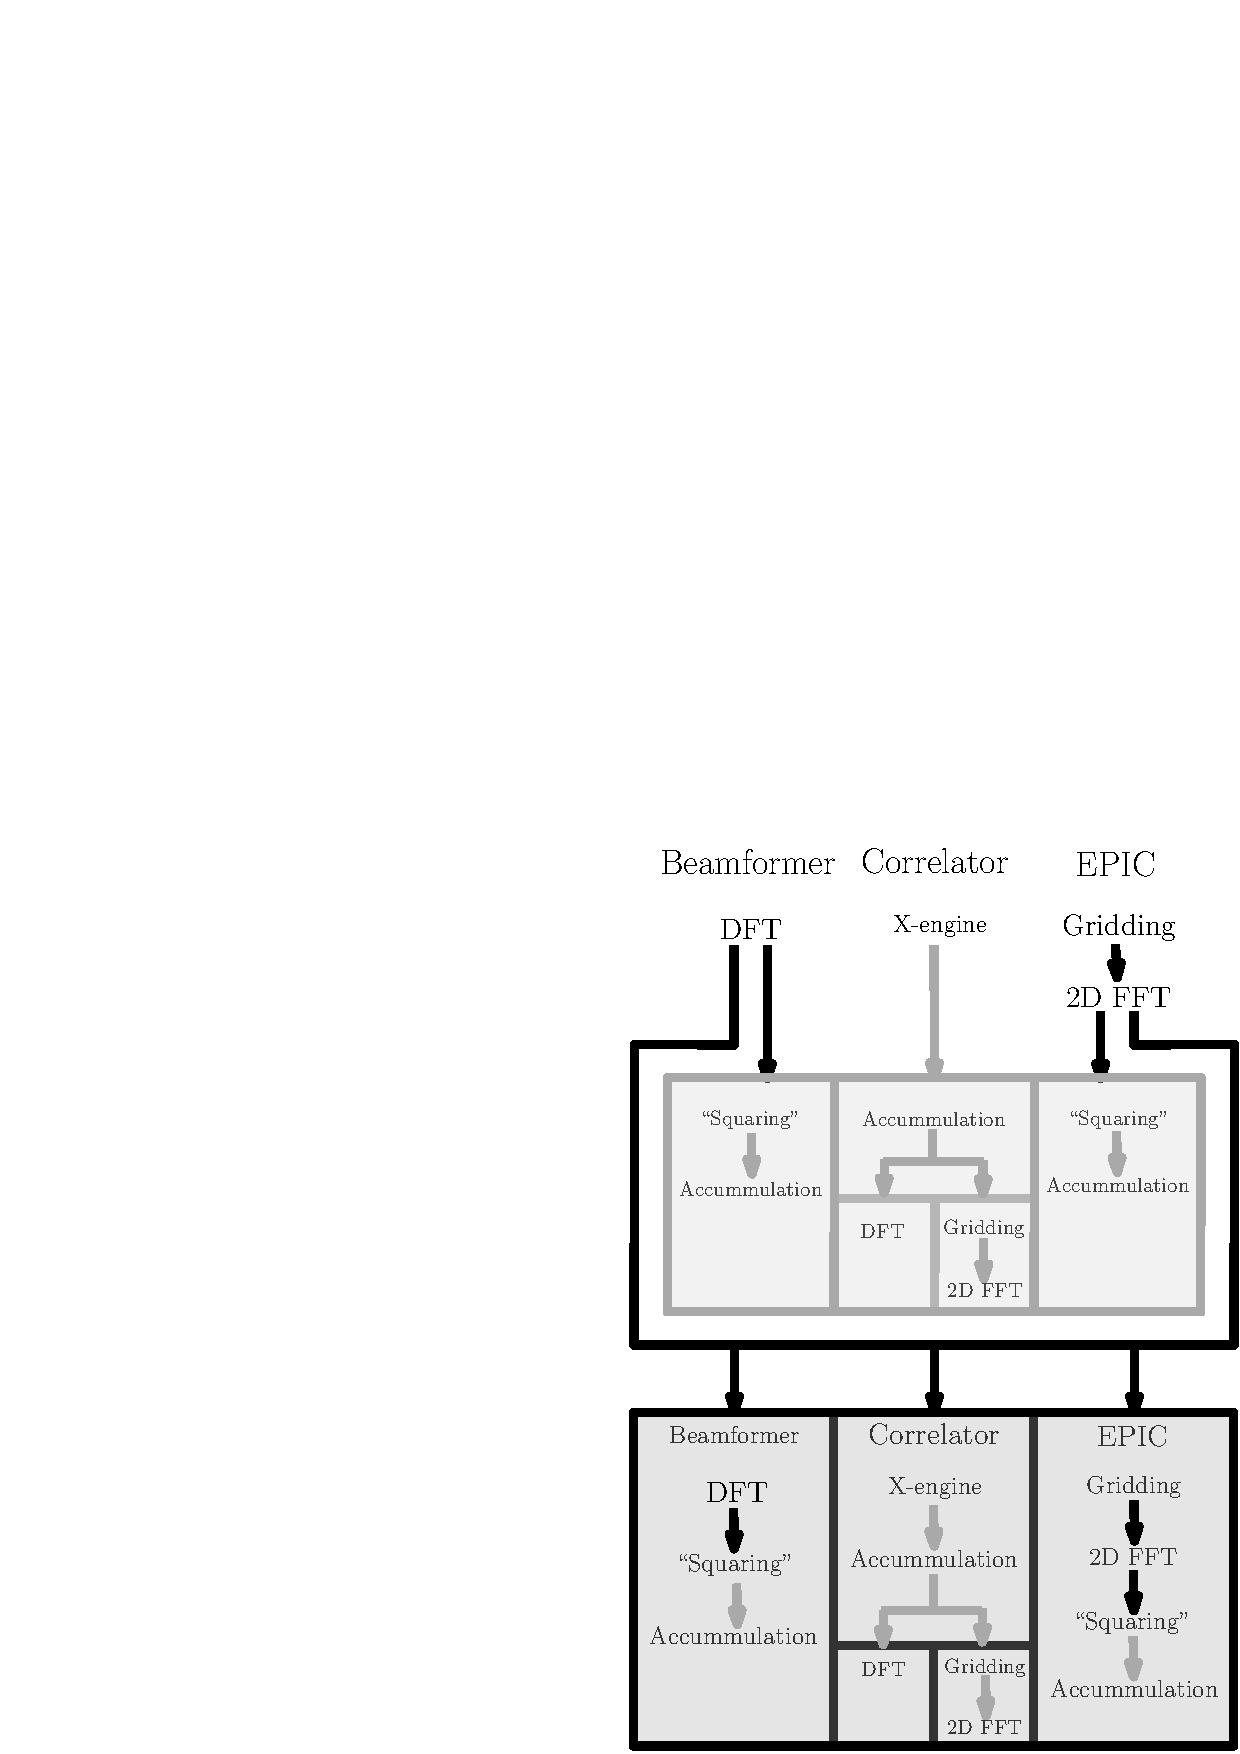
\includegraphics[width=\linewidth]{fig_01.pdf}
\caption{
\label{fig:hybrid-architectures-cost-schematic}}
\end{figure*}

\section{Intra-station Imaging Architectures} \label{sec:intra-station-arch}

We first describe the first stage, namely, intra-station architectures that form the basis for both approaches. This first stage essentially synthesises station-scale apertures with simultaneous, multiple virtual pointings. These station-scale apertures from the first stage will act as fundamental elements for the second stage of inter-station processing. We will use $a_m$ to denote element, $a$, in station, $m$.

\subsection{Voltage Beamforming (BF)}

The calibrated electric fields recorded by individual elements within a station can be phase-coherently superposed towards any desired direction as
\begin{align}
    \widetilde{\mathcal{E}}_m^\alpha(\hat{\boldsymbol{s}}_k) &= \sum_{a_m} \sum_p  \widetilde{\mathcal{W}}_{a_m}^{{p\alpha}^*}(\hat{\boldsymbol{s}}_k) \, \widetilde{E}_{a_m}^p \, e^{i\frac{2\pi}{\lambda} \hat{\boldsymbol{s}}_k\cdot\boldsymbol{r}_{a_m}} \, , \label{eqn:intra-station-pol-hol-img-expl}
\end{align}
where, $\hat{\boldsymbol{s}}_k$ denotes the direction of beam, $k$, towards which the measurements are phase-coherently superposed, $\widetilde{E}_{a_m}^{p}$ represents the calibrated and potentially noise-weighted electric field measured by the station element $a_m$, and $\widetilde{\mathcal{W}}_{a_m}^{{p\alpha}^*}(\hat{\boldsymbol{s}}_k)$ denotes a complex-valued directional weighting\footnote{One can choose $\widetilde{\mathcal{W}}_{a_m}^{p\alpha}(\hat{\boldsymbol{s}}_k)=\mathcal{W}_{a_m}^{p\alpha}(\hat{\boldsymbol{s}}_k)$, the directional electric field sensitivity, if the signal-to-noise ratio is to be optimised. But it can also be generically chosen depending on the property desired of the estimator \cite[][]{Morales2011}.} applied to the station element. This beamforming step has to be executed at a cadence of $\delta t$. 

The polarised intensity in a pixel is then obtained by
\begin{align}
    \widetilde{\mathcal{I}}^{\alpha\beta}_m(\hat{\boldsymbol{s}}_k) &= \left\langle \widetilde{\mathcal{E}}_m^\alpha(\hat{\boldsymbol{s}}_k) \,  \widetilde{\mathcal{E}}_m^{\beta^*}(\hat{\boldsymbol{s}}_k) \right\rangle \, , \label{eqn:intra-station-opt-pol-img-outprod}
\end{align}
where, the angular brackets denote a temporal averaging across an interval of $\Delta t$. Even though it is an outer product over the polarisation axis, we will refer to it as a ``squaring'' operation hereafter for convenience because of what it reduces to if only a single polarisation was measured. 

The solid angle of the beamformed pixel using the intra-station data is given by $\Omega_s \simeq (\lambda/D_\textrm{s})^2$. Beamforming can be applied to all independent beams ($n_\textrm{bs}$) filling the field of view, whose solid angle is $\Omega_a \simeq (\lambda/D_\textrm{a})^2$. Thus, $n_\textrm{bs} \simeq \Omega_\textrm{a}/\Omega_\textrm{s}=(D_\textrm{s}/D_\textrm{a})^2$. 

The computational cost budget consists of the following components. Beamforming $N_\textrm{a/s}$ element polarised voltages (with $n_\textrm{p}$ polarisations) towards $n_\textrm{bs}$ beams on sky as per Equation~(\ref{eqn:intra-station-pol-hol-img-expl}) requires $n_\textrm{p} n_\textrm{bs} N_\textrm{a/s}$ CMACs to get one polarised voltage on sky per station per channel. To get $n_\textrm{p}$ polarised voltages from beamforming, it requires $n_\textrm{p}^2 n_\textrm{bs} N_\textrm{a/s}$ CMACs amounting to $8 n_\textrm{p}^2 n_\textrm{bs} N_\textrm{a/s}/\delta t$ FLOPS per station per channel. 

Converting polarised beamformed voltages on the sky to Stokes intensities and temporally averaging them as per Equation~(\ref{eqn:opt-pol-corr-img-outprod}) requires $n_\textrm{p}^2$ complex "squaring" (complex products) and subsequent complex additions for each of the complex polarised voltage beams, and therefore $n_\textrm{p}^2 n_\textrm{bs}$ CMACs per station channel, amounting to $8 n_\textrm{p}^2 n_\textrm{bs}$ FLOPS per station per channel. Hence, the net rate corresponding to beamforming, squaring, and averaging is $8 n_\textrm{p}^2 (D_\textrm{s}/D_\textrm{a})^2 (N_\textrm{a/s}+1)/\delta t$ FLOPS per station per channel. 

% \begin{figure*}
% \centering
% \subfloat[][Two-dimensional slices \label{fig:multidim-incoherent-compcost-BF-SKA-low}]{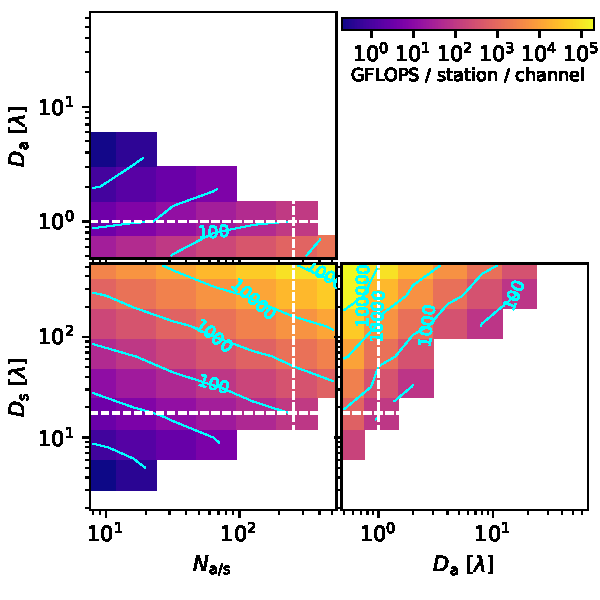
\includegraphics[width=0.4\textwidth]{figures/multidim_beamformer_dft_cost_analysis_SKA1-low.pdf}}
% \subfloat[][One-dimensional slices\label{fig:1D-incoherent-compcost-BF-SKA-low}]{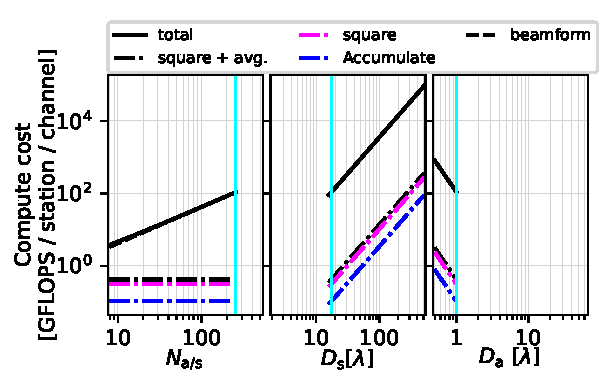
\includegraphics[width=0.58\textwidth]{figures/1D_beamformer_dft_cost_analysis_SKA1-low.pdf}}
% \caption{(Left): Two-dimensional slices of the computational cost for coherent-incoherent imaging using station-level voltage beamforming for \texttt{SKA-low-core}, \texttt{SKA-low}, \texttt{Aus-VLBA-low}, and \texttt{IC-VLBA-low}. Cyan contours  \label{fig:incoherent-compcost-BF-SKA-low}}
% \end{figure*}

\begin{figure}
\includegraphics[width=\linewidth]
% {figures/1D_beamformer_dft_cost_analysis_SKA1-low.pdf}
{figures/1D_beamformer_dft_per_pixel_cost_analysis_LAMBDA-I.pdf}
% 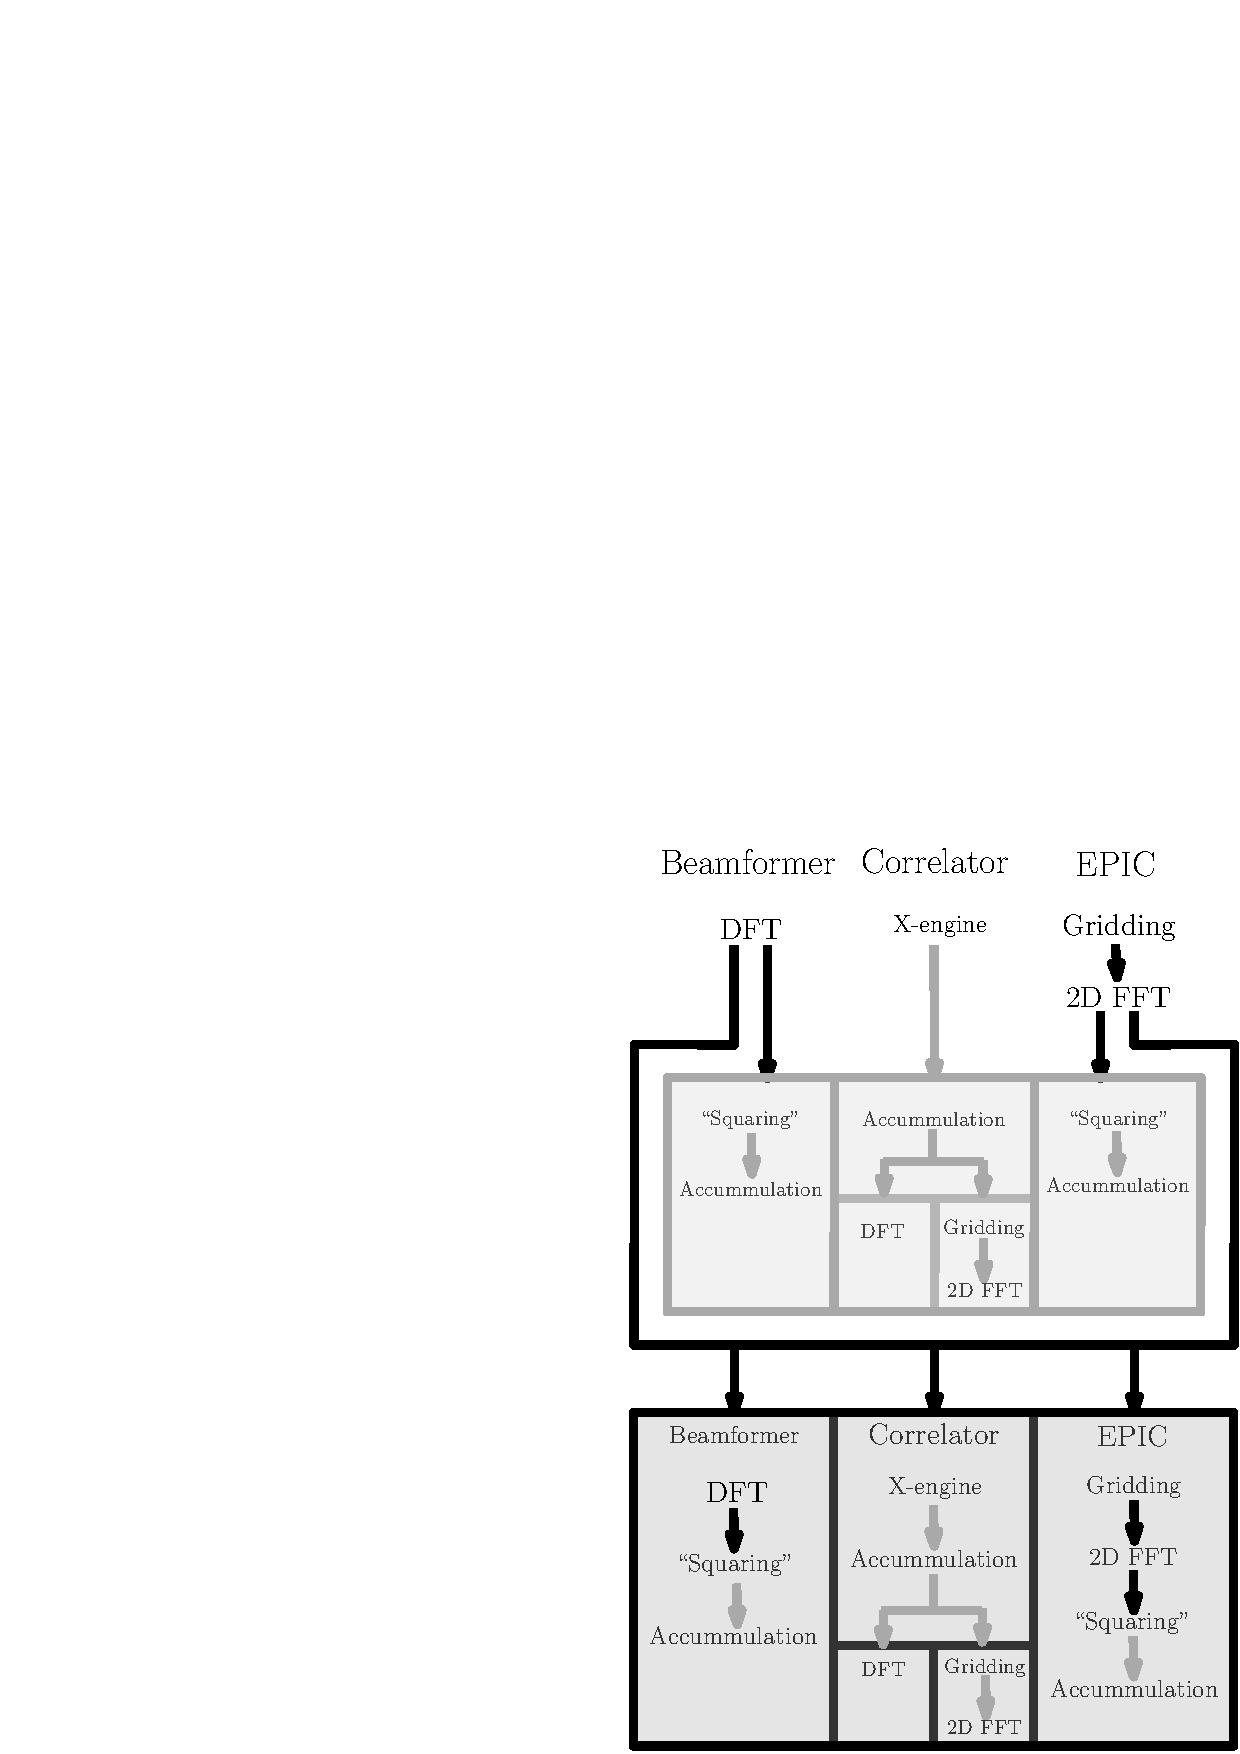
\includegraphics[width=\linewidth]{fig_01.pdf}
\caption{A breakdown of the computational cost density function over the instrument parameters for \texttt{LAMBDA-I} using the voltage beamforming architecture at the station level.
\label{fig:1D-incoherent-compcost-BF-LAMBDA-I}}
\end{figure}

\begin{figure}
\includegraphics[width=\linewidth]
% {figures/multidim_beamformer_dft_cost_analysis_SKA1-low.pdf}
{figures/multidim_beamformer_dft_per_pixel_cost_analysis_LAMBDA-I.pdf}
% 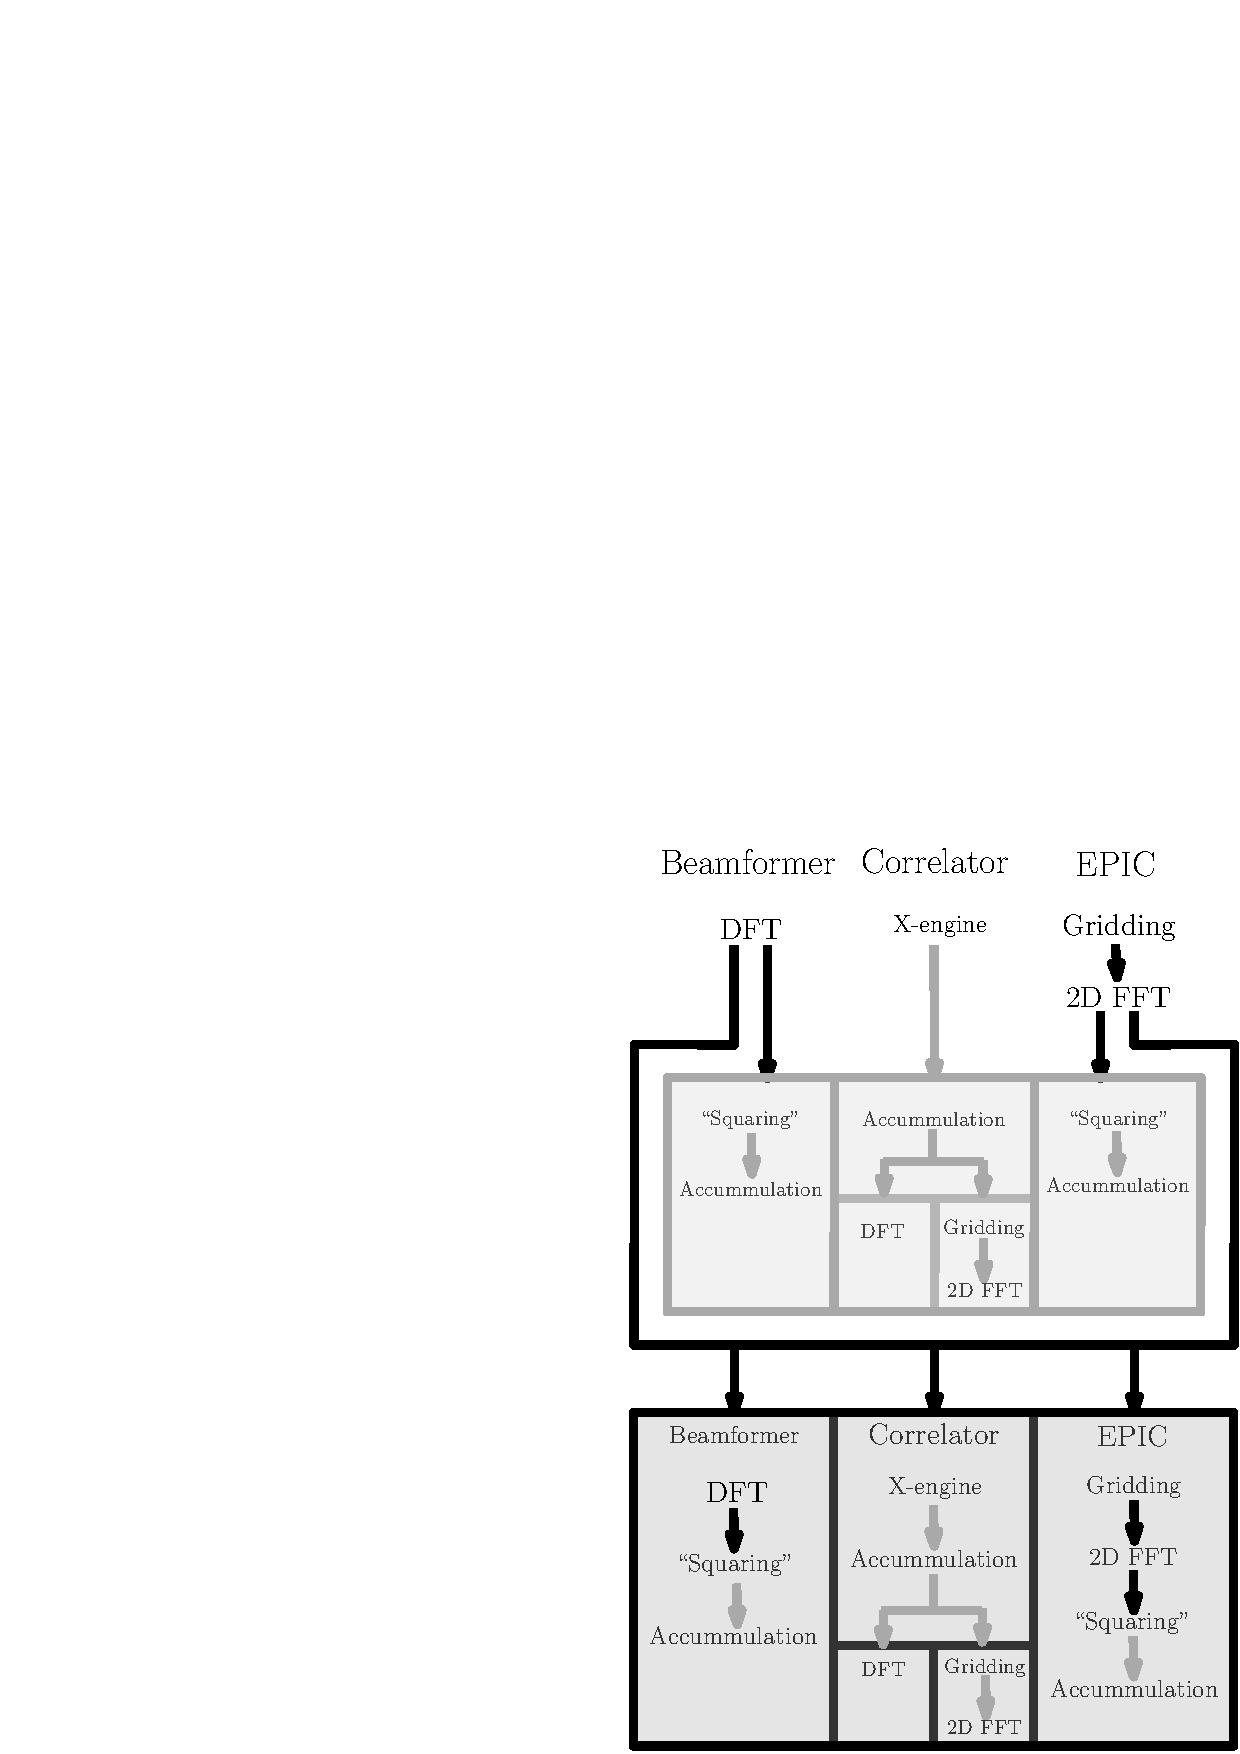
\includegraphics[width=\linewidth]{fig_01.pdf}
\caption{A multi-dimensional view of the net computational cost density function over the instrumental parameters for \texttt{LAMBDA-I} using the voltage beamforming architecture at the station level.
\label{fig:multidim-incoherent-compcost-BF-LAMBDA-I}}
\end{figure}

\subsection{E-field Parallel Imaging Correlator (EPIC)}

A simultaneous beamforming filling the entire field of view can also be achieved by a two-dimensional spatial Fast Fourier Transform (FFT) of the measurements on the aperture plane. This can be enabled even for an irregular layout of station elements by gridding the calibrated electric fields measured by the station elements. The Optimal Map Making formalism \citep[OMM;][]{Tegmark+1997a} formalism adopted by \citet{Morales2011} is the basis of the architecture called E-field Parallel Imaging Correlator \cite[EPIC;][]{Thyagarajan+2017},
\begin{align}
    \widetilde{\mathcal{E}}_m^\alpha(\hat{\boldsymbol{s}}_k) &= \sum_j \delta^2 \boldsymbol{r}_j \, e^{i\frac{2\pi}{\lambda} \hat{\boldsymbol{s}}_k\cdot\boldsymbol{r}_j} \left(\sum_{a_m} \sum_p \widetilde{W}_{a_m}^{p\alpha*}(\boldsymbol{r}_j-\boldsymbol{r}_{a_m}) \, \widetilde{E}_{a_m}^p \right) \, , \label{eqn:intra-station-pol-hol-img-epic}
\end{align}
whose equivalent linear algebraic representation is 
\begin{align}
    \widetilde{\boldsymbol{\mathcal{E}}}_{[m,\alpha,\hat{\boldsymbol{s}}]} &= \mathbf{F}^\textrm{H}_{[\hat{\boldsymbol{s}}\leftarrow \boldsymbol{r}]}\,\widetilde{\mathbf{W}}^\textrm{H}_{[\alpha,\boldsymbol{r}\leftarrow p,\boldsymbol{r}_{a_m}]}\,\widetilde{\mathbf{E}}_{[p,\boldsymbol{r}_{a_m}]} \, . \label{eqn:intra-station-pol-hol-img-epic-LA}
\end{align}

Application of the FFT will have the effect of simultaneously beamforming over the entire field of view, $\Omega_\textrm{a}$. The convolution with $\widetilde{W}_{a_m}^{p\alpha*}(\boldsymbol{r})$ has two purposes. Firstly, it can be chosen to optimise specific properties in the synthesised image. For example, choosing $\widetilde{W}_{a_m}^{p\alpha}(\boldsymbol{r})=W_{a_m}^{p\alpha*}(\boldsymbol{r})$ will optimise the signal-to-noise ratio in the image. Secondly, it also acts as gridding convolution transforming data from discrete and arbitrary locations onto a regular grid, thereby facilitating the application of a two-dimensional spatial FFT. 

The polarised intensity on $\mathbb{S}$ is again given by Equation~(\ref{eqn:intra-station-opt-pol-img-outprod}), which is expressed linear algebraically as
\begin{align}
    \widetilde{\mathbf{I}}_{[m,\alpha\beta,\hat{\boldsymbol{s}}]} &= \left\langle \widetilde{\boldsymbol{\mathcal{E}}}_{[m,\alpha,\hat{\boldsymbol{s}}]} \bigotimes_{\alpha\beta} \widetilde{\boldsymbol{\mathcal{E}}}_{[m,\beta,\hat{\boldsymbol{s}}]}^* \right\rangle \, , \label{eqn:intra-station-opt-polarimetric-direct-img-LA}    
\end{align}
where, the outer product is performed over polarisation indices, $\alpha$ and $\beta$. 

The EPIC architecture has been implemented on the Long Wavelength Array station in Sevilleta (NM, USA) \cite{Kent+2019,Kent+2020,Krishnan+2023} using a GPU framework and offered to the user community commensally.  

\begin{figure}
\includegraphics[width=\linewidth]
% {figures/1D_epic_cost_analysis_SKA1-low.pdf}
{figures/1D_epic_per_pixel_cost_analysis_LAMBDA-I.pdf}
% 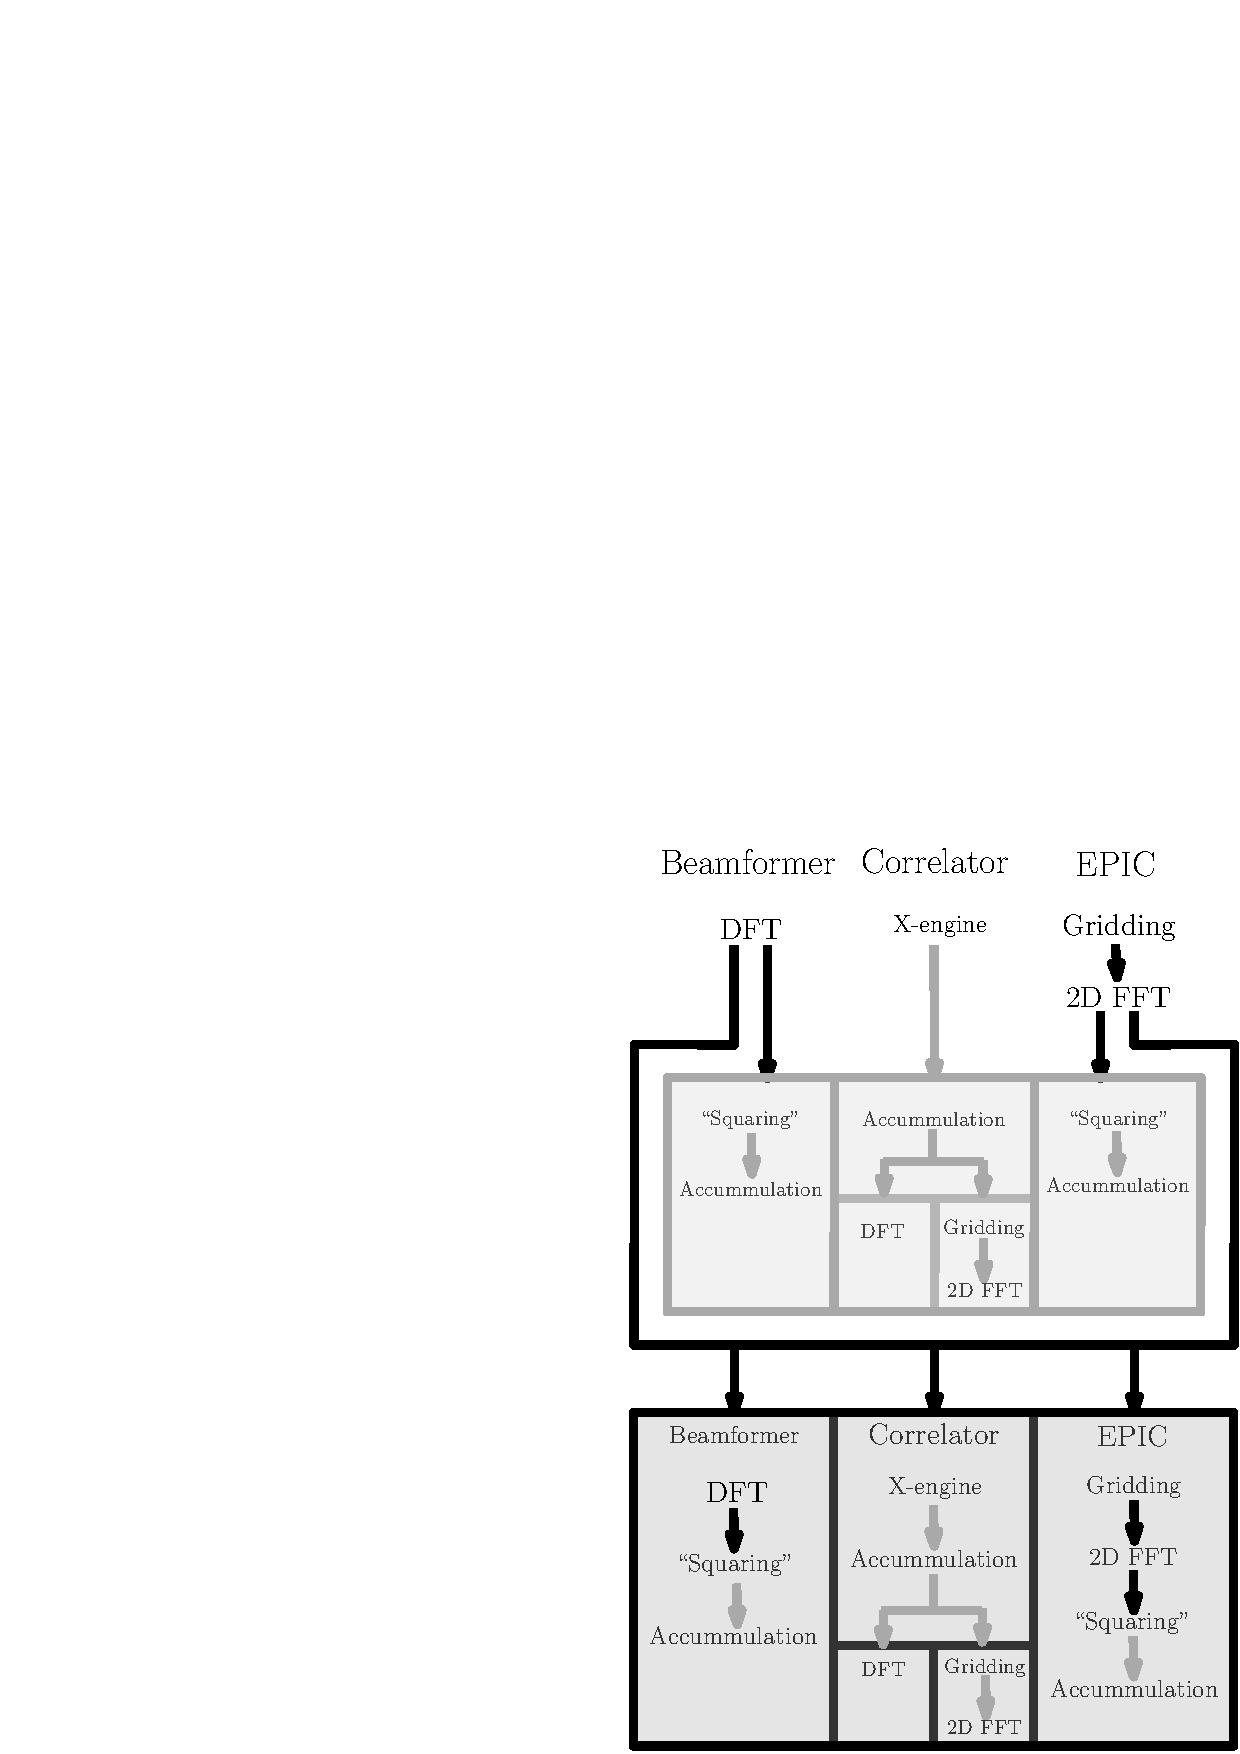
\includegraphics[width=\linewidth]{fig_01.pdf}
\caption{
\label{fig:1D-incoherent-compcost-EPIC-LAMBDA-I}}
\end{figure}

\begin{figure*}
\centering
\subfloat[][Two-dimensional slices \label{fig:multidim-incoherent-compcost-EPIC-LAMBDA-I}]{\includegraphics[width=0.48\textwidth]
% {figures/multidim_epic_cost_analysis_SKA1-low.pdf}
{figures/multidim_epic_per_pixel_cost_analysis_LAMBDA-I.pdf}
}
\subfloat[][Two-dimensional slices (relative)\label{fig:multidim-incoherent-relative-compcost-EPIC-LAMBDA-I}]{\includegraphics[width=0.48\textwidth]
% {figures/multidim_epic_relative_cost_analysis_SKA1-low.pdf}
{figures/multidim_epic_relative_cost_analysis_LAMBDA-I.pdf}
} 
\caption{(Left): Two-dimensional slices of the computational cost for coherent-incoherent imaging using station-level EPIC for \texttt{SKA-low}. Cyan contours  \label{fig:incoherent-compcost-EPIC-LAMBDA-I}}
\end{figure*}


\subsection{Correlator Beamforming (XBF)}

Calibrated visibilities, $\widetilde{V}_{a_m b_m}^{pq}$, in a station, $m$, can be written as 
\begin{align}
    V_{a_m b_m}^{pq} &= \bigl\langle E_{a_m}^p \, E_{b_m}^{q*}\bigr\rangle \label{eqn:intra-station-pol-visibilities}
\end{align}
which can be beamformed through a discrete Fourier transform (DFT) to obtain intensities in any desired direction, $\boldsymbol{s}_k$, as
\begin{align}
    \widetilde{\mathcal{I}}_m^{\alpha\beta}(\hat{\boldsymbol{s}}_k) 
    &= \sum_{a_m,b_m} \sum_{p,q} \widetilde{\mathcal{B}}_{a_m b_m}^{*pq;\alpha\beta}(\hat{\boldsymbol{s}}_k) \, \widetilde{V}_{a_m b_m}^{pq} \,  e^{i\frac{2\pi}{\lambda} \hat{\boldsymbol{s}}_k\cdot\Delta\boldsymbol{r}_{a_m b_m}} \, , \label{eqn:intra-station-pol-xbf-img-expl} 
\end{align}
where, $a_m$ and $b_m$ are elements $a$ and $b$ in station $m$. $\widetilde{\mathcal{B}}_{a_m b_m}^{*pq;\alpha\beta}(\hat{\boldsymbol{s}}_k)$ denotes a complex-valued directional weighting applied to the calibrated visibility and can be chosen to produce images with desired characteristics \citep{Masui+2019}. 
% This correlation beamforming step can be executed at a cadence of $\Delta t$. However, the correlations that produce visibilities must still be executed on timescales of $\delta t$. Like voltage beamforming, the number of independent beams filling the field of view is $n_\textrm{bs} \simeq (D_\textrm{s}/D_\textrm{a})^2$. 

The computational cost budget consists of the following components. The formation of polarimetric visibilities and their accumulations requires $n_\textrm{p}^2 N_\textrm{a/s} (N_\textrm{a/s}-1)/2$ complex multiplications and complex additions, respectively, per station per channel at a cadence of $\delta t$. These accumulated visibilities will be further averaged across stations but on a slower cadence of $\Delta t$. However, in order to obtain stationwise image intensities, we will not consider averaging across stations. Thus, the computational cost of forming polarimetric visibilities and their accumulations per station per channel is $4 n_\textrm{p}^2 N_\textrm{a/s} (N_\textrm{a/s}-1)/(\delta t)$ FLOPS. The accumulated visibilities from a station can be beamformed towards $n_\textrm{bs}\simeq (D_\textrm{s}/D_\textrm{a})^2$ sky locations using a DFT to obtain Stokes intensities. This DFT beamforming performs $n_\textrm{p}^2 N_\textrm{a/s} (N_\textrm{a/s}-1) (D_\textrm{s}/D_\textrm{a})^2 /2$ CMACs at a slower cadence of $\Delta t$. Hence, the net computational cost for DFT beamforming of visibilities across the field of view per station per channel is 
\begin{align}
    C_\textrm{XBF} &= 4 n_\textrm{p}^2 \, N_\textrm{a/s} (N_\textrm{a/s}-1) \left[\frac{1}{\delta t} + \frac{\left(D_\textrm{s}/D_\textrm{a}\right)^2}{\Delta t} \right] \, . \label{eqn:cost-XBF}
\end{align}

\begin{figure}
\includegraphics[width=\linewidth]
% {figures/1D_xcor_dft_cost_analysis_SKA1-low.pdf}
{figures/1D_xcor_dft_per_pixel_cost_analysis_LAMBDA-I.pdf}
% 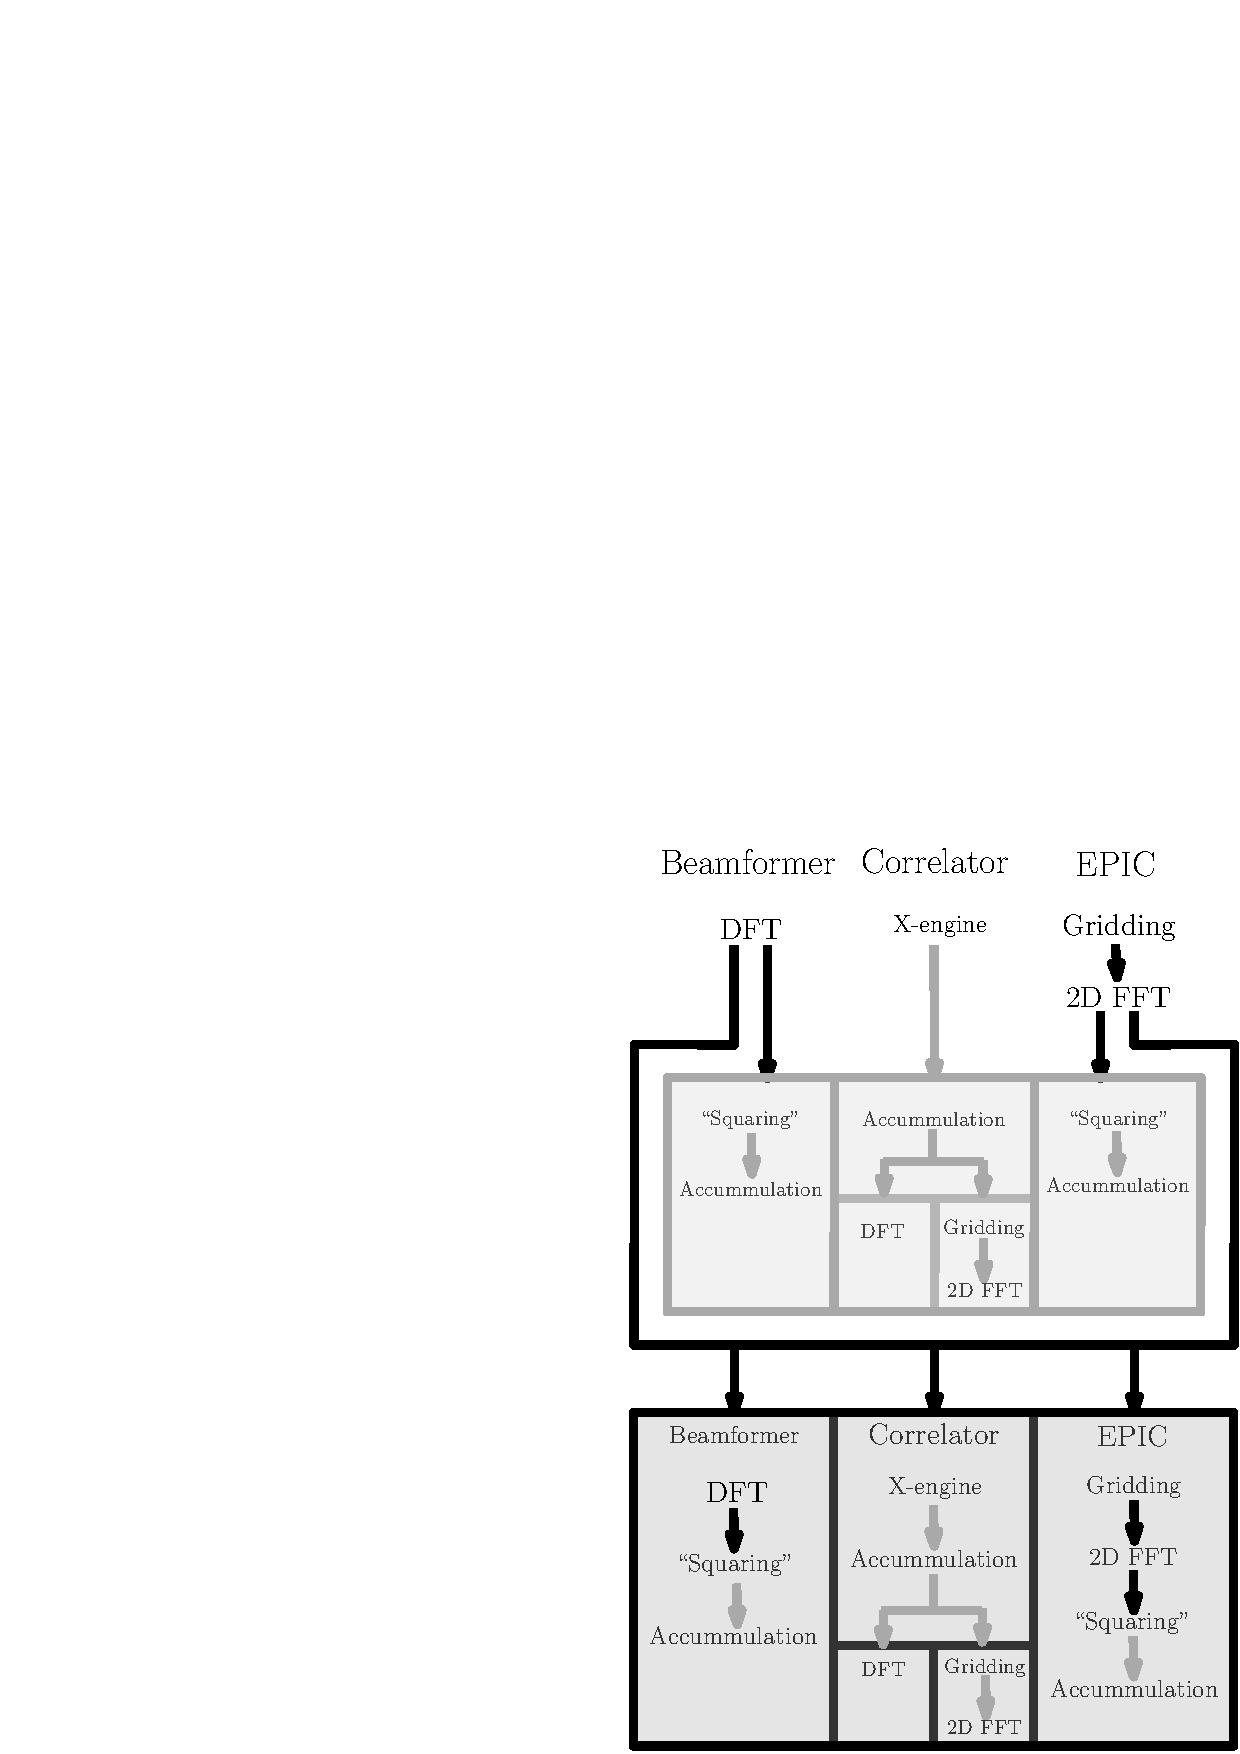
\includegraphics[width=\linewidth]{fig_01.pdf}
\caption{
\label{fig:1D-incoherent-compcost-XBF-LAMBDA-I}}
\end{figure}

\begin{figure*}
\centering
\subfloat[][Two-dimensional slices \label{fig:multidim-incoherent-compcost-XBF-LAMBDA-I}]
{\includegraphics[width=0.48\textwidth]
% {figures/multidim_xcor_dft_cost_analysis_SKA1-low.pdf}
{figures/multidim_xcor_dft_per_pixel_cost_analysis_LAMBDA-I.pdf}
}
\subfloat[][Two-dimensional slices (relative)\label{fig:multidim-incoherent-relative-compcost-XBF-LAMBDA-I}]
{\includegraphics[width=0.48\textwidth]
% {figures/multidim_xcor_dft_relative_cost_analysis_SKA1-low.pdf}
{figures/multidim_xcor_dft_relative_cost_analysis_LAMBDA-I.pdf}
}
\caption{(Left): Two-dimensional slices of the computational cost for coherent-incoherent imaging using a DFT of station-level cross-correlations for \texttt{SKA-low-core}, \texttt{SKA-low}, \texttt{Aus-VLBA-low}, and \texttt{IC-VLBA-low}. Cyan contours  \label{fig:incoherent-compcost-XBF-LAMBDA-I}}
\end{figure*}

\subsection{Correlation and FFT (XFFT)}

Here, the calibrated station visibilities, $\widetilde{V}_{a_m b_m}^{pq}$, in Equation~(\ref{eqn:intra-station-pol-visibilities}) are gridded and Fourier transformed using an FFT rather than the discrete Fourier transform of correlator beamforming. Mathematically, it is similar to the operations performed on calibrated electric fields from the elements in EPIC, with two key differences -- (1) the calibrated visibilities can be accumulated and allowed for Earth rotation and bandwidth synthesis, (2) the gridding and spatial Fourier transform operates on visibilities rather than electric fields, and (2) the spatial Fourier transform can occur on a slower cadence of $\Delta t$ or the calibration timescale, whichever is shorter. needs to happen 

The optimal map-making (OMM) formalism \citep{Tegmark1997a} provides a lossless and optimal (least-squares) solution, which in the radio interferometric context is often referred to as the ``dirty image'' \citep{TMS2017,SIRA-II}, and can be expressed linear algebraically as \citep{Bhatnagar+2008,Morales+2009}:
\begin{align}
    \widetilde{\mathbf{I}}_{[m,\alpha\beta,\hat{\boldsymbol{s}}]} &=  \mathbf{F}^\textrm{H}_{[\hat{\boldsymbol{s}}\leftarrow\Delta\boldsymbol{r}]}\,\widetilde{\mathbf{B}}^\textrm{H}_{[\alpha\beta,\Delta\boldsymbol{r}\leftarrow pq,\Delta\boldsymbol{r}_{a_m b_m}]} \nonumber\\ 
    &\qquad \mathbf{N}^{-1}_{[\Delta\boldsymbol{r}_{a_m b_m}\leftarrow\Delta\boldsymbol{r}_{a_m b_m}]}\,\widehat{\mathbf{V}}_{[pq,\Delta\boldsymbol{r}_{a_m b_m}]} \label{eqn:intra-station-opt-pol-corr-image}
    % &= \mathbf{F}^\textrm{H}_{[\hat{\boldsymbol{s}}\leftarrow\Delta\boldsymbol{r}]}\,\mathbf{B}^\textrm{H}_{[\Delta\boldsymbol{r}\leftarrow\Delta\boldsymbol{r}_{a_m b_m}]}\,\mathbf{N}^{-1}_{[\Delta\boldsymbol{r}_{a_m b_m}\leftarrow\Delta\boldsymbol{r}_{a_m b_m}]} \nonumber\\ 
    % &\qquad\qquad\qquad \vect\left(\Bigl\langle\widehat{\mathbf{E}}_{[\boldsymbol{r}_{a_m}]}\widehat{\mathbf{E}}^\textrm{H}_{[\boldsymbol{r}_{b_m}]}\Bigl\rangle\right)_{[\Delta\boldsymbol{r}_{a_m b_m}]} \, . \label{eqn:opt-copolar-corr-image}
\end{align}
The subscript, $m$, on the left hand side denotes that the image was made using measurements within the station, $m$. The inversion operation above takes a column vector of calibrated visibilities, $\widehat{\mathbf{V}}_{[pq,\Delta\boldsymbol{r}_{a_m b_m}]}\coloneqq \vect\left(\Bigl\langle\widehat{\mathbf{E}}_{[p,\boldsymbol{r}_{a_m}]}\widehat{\mathbf{E}}^\textrm{H}_{[q,\boldsymbol{r}_{b_m}]}\Bigl\rangle\right)$ at element spacings, $\Delta\boldsymbol{r}_{a_m b_m}$, in station $m$, weights them by the inverse noise covariance, $\mathbf{N}_{[\Delta\boldsymbol{r}_{a_m b_m}\leftarrow\Delta\boldsymbol{r}_{a_m b_m}]}\coloneqq \langle \boldsymbol{n}_{[\Delta\boldsymbol{r}_{a_m b_m}]}\boldsymbol{n}^\textrm{H}_{[\Delta\boldsymbol{r}_{a_m b_m}]}\rangle$, then weights and projects this inverse noise-covariance weighted vector of visibilities onto a finely sampled grid denoted by $\Delta\boldsymbol{r}$ using the gridding operator $\widetilde{\mathbf{B}}^\textrm{H}_{[\alpha\beta,\Delta\boldsymbol{r}\leftarrow pq,\Delta\boldsymbol{r}_{a_m b_m}]}$, and inverse-Fourier transforms using $\mathbf{F}^\textrm{H}_{[\hat{\boldsymbol{s}}\leftarrow\Delta\boldsymbol{r}]}$ to obtain the estimate of the vector of pixelized intensities, $\widetilde{\mathbf{I}}_{[m,\alpha\beta,\hat{\boldsymbol{s}}]}$, on $\mathbb{S}$ corresponding to station, $m$. 

The purpose of $\widetilde{\mathbf{B}}^\textrm{H}_{[\alpha\beta,\Delta\boldsymbol{r}\leftarrow pq,\Delta\boldsymbol{r}_{a_m b_m}]}$ is similar \citep{Morales+2009,Cornwell+2008} to its counterpart gridding operator in the EPIC architecture \citep{Morales2011}. 
% implies the following. First, if $\widetilde{\mathbf{B}}^\textrm{H}=\mathbf{B}^\textrm{H}$ (assumed hereafter, unless specified), then the inversion is lossless and optimal, minimizing noise and the reconstruction error \citep{Tegmark1997a}. This form is very similar to a matched filter. Second, it transforms the inverse noise covariance weighted visibilities at arbitrary locations, $\Delta\boldsymbol{r}_{a_m b_m}$, to finely sampled locations, $\Delta\boldsymbol{r}$, on a grid. If the grid is uniformly sampled, it facilitates efficient inverse Fourier transform using Fast Fourier Transform (FFT) algorithms. 
Noting that the optimal inversion is weighted by $\widetilde{\mathbf{B}}^\textrm{H}$, which is the conjugate of that in the RIME in Equation~(\ref{eqn:RIME-LA}), the phase introduced by the instrument is cancelled out precisely during the inversion. However, the amplitude is not. Hence, the inverted image, $\widetilde{\mathbf{I}}_{[\hat{\boldsymbol{s}}]}$, is attenuated relative to the true image, $\mathbf{I}_{[m,\alpha\beta,\hat{\boldsymbol{s}}]}$, by a factor that is square of the interferometer's angular power pattern \citep{Cornwell+2008,Morales+2009}, once due to $\mathbf{B}_{[pq,\Delta\boldsymbol{r}_{a_m b_m}\leftarrow \alpha\beta,\Delta\boldsymbol{r}]}$ in Equation~(\ref{eqn:RIME-LA}) (inherent in the measurement) and once more due to $\widetilde{\mathbf{B}}^\textrm{H}_{[\alpha\beta,\Delta\boldsymbol{r}\leftarrow pq,\Delta\boldsymbol{r}_{a_m b_m}]}$ in Equation~(\ref{eqn:intra-station-opt-pol-corr-image}). 

The computational cost consists of forming the visibilities and accumulating them, gridding them using the gridding kernel and accumulating them on the grid in case of overlapping data, and spatial FFT to obtain the polarimetric images. 

% \begin{table*}[htb!]
% \normalsize
% \begin{threeparttable}
% \caption{Computational budget of intra-station coherent imaging architectures}
% \label{tab:intra-station-coherent-imaging}
% \begin{tabular}{ccccc}
% % \begin{tabularx}{\textwidth}{ccccc}
% \toprule
% \headrow Intra-station & Components & Equation & FLOP count & Timescale \\
% architecture & & & (per station per channel) & \\ 
% \midrule\midrule
% VBF & Beamforming & \ref{eqn:intra-station-pol-hol-img-expl} & $8 n_\textrm{p}^2 N_\textrm{a/s} \left(\frac{D_\textrm{s}}{D_\textrm{a}}\right)^2$ & $\delta t$ \\
% & Squaring & \ref{eqn:intra-station-opt-pol-img-outprod} & $6 n_\textrm{p}^2 \left(\frac{D_\textrm{s}}{D_\textrm{a}}\right)^2$ & $\delta t$ \\
% & Accumulation & \ref{eqn:intra-station-opt-pol-img-outprod} & $2 n_\textrm{p}^2 \left(\frac{D_\textrm{s}}{D_\textrm{a}}\right)^2$ & $\delta t$ \\
% \midrule
% EPIC & Gridding & \ref{eqn:intra-station-pol-hol-img-epic-LA} & $6 n_\textrm{p}^2 N_\textrm{a/s} N_\textrm{ka}$ & $\delta t$ \\
% & FFT & \ref{eqn:intra-station-pol-hol-img-epic-LA} & $8 n_\textrm{p} \frac{r}{\log_2 r} \left(\gamma_\textrm{s}\frac{D_\textrm{s}}{D_\textrm{a}}\right)^2\log_2\left(\gamma_\textrm{s}\frac{D_\textrm{s}}{D_\textrm{a}}\right)^2$ & $\delta t$ \\
% & Squaring & \ref{eqn:intra-station-opt-polarimetric-direct-img-LA} & $6 n_\textrm{p}^2 \left(\gamma_\textrm{s} \frac{D_\textrm{s}}{D_\textrm{a}}\right)^2$ & $\delta t$ \\
% & Accumulation & \ref{eqn:intra-station-opt-polarimetric-direct-img-LA} & $2 n_\textrm{p}^2 \left(\gamma_\textrm{s} \frac{D_\textrm{s}}{D_\textrm{a}}\right)^2$ & $\delta t$ \\
% \midrule
% XBF & Correlator & \ref{eqn:intra-station-pol-visibilities} & $6 n_\textrm{p}^2 N_\textrm{a/s} (N_\textrm{a/s}-1)/2$ & $\delta t$ \\
% & Accumulation & \ref{eqn:intra-station-pol-visibilities} & $2 n_\textrm{p}^2 N_\textrm{a/s} (N_\textrm{a/s}-1)/2$ & $\delta t$ \\
% & DFT & \ref{eqn:intra-station-pol-xbf-img-expl} & $8 n_\textrm{p}^2 \left(\frac{D_\textrm{s}}{D_\textrm{a}}\right)^2 N_\textrm{a/s} (N_\textrm{a/s}-1)/2$ & $\Delta t$ \\
% \midrule
% XFFT & Correlator & \ref{eqn:intra-station-pol-visibilities} & $6 n_\textrm{p}^2 N_\textrm{a/s} (N_\textrm{a/s}-1)/2$ & $\delta t$ \\
% & Accumulation & \ref{eqn:intra-station-pol-visibilities} & $2 n_\textrm{p}^2 N_\textrm{a/s} (N_\textrm{a/s}-1)/2$ & $\delta t$ \\
% & Gridding & \ref{eqn:intra-station-opt-pol-corr-image} & 8$n_\textrm{p}^4 (2^2 N_\textrm{ka}) N_\textrm{a/s} (N_\textrm{a/s}-1)/2$ & $\Delta t$ \\
% & FFT & \ref{eqn:intra-station-opt-pol-corr-image} & $8 n_\textrm{p}^2 \frac{r}{\log_2 r} \left(\frac{D_\textrm{s}}{D_\textrm{a}}\right)^2\log_2\left(\frac{D_\textrm{s}}{D_\textrm{a}}\right)^2$ & $\Delta t$ \\
% % \midrule
% % Three & Four&three three\tnote{b} &four & & \\
% \bottomrule
% % \end{tabularx}
% \end{tabular}
% \begin{tablenotes}[hang]
% % \item[]Table note
% \item[a]Array filling factor, $\,f_\textrm{A}=N_\textrm{s}\,(D_\textrm{s}/D_\textrm{A})^2$
% % \item[b]Station filling factor, $\,f_\textrm{s}=N_\textrm{a/s}\,(D_\textrm{a}/D_\textrm{s})^2$
% \end{tablenotes}
% \end{threeparttable}
% \end{table*}

% \subsubsection{Correlator Beamforming (XBF)}

% \cite{Masui+2019}

% \begin{figure*}
% \centering
% \subfloat[][Two-dimensional slices \label{fig:multidim-incoherent-compcost-XBF-SKA-low}]{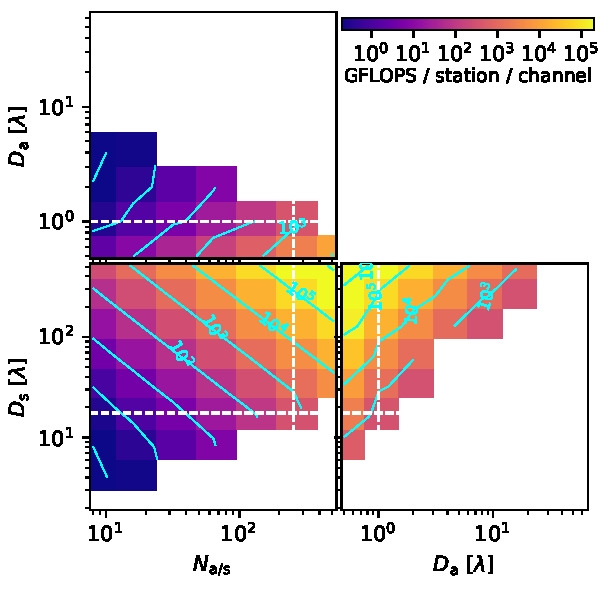
\includegraphics[width=0.48\textwidth]{figures/multidim_xcor_dft_cost_analysis_SKA1-low.pdf}}
% \subfloat[][Two-dimensional slices (relative)\label{fig:multidim-incoherent-relative-compcost-XBF-SKA-low}]{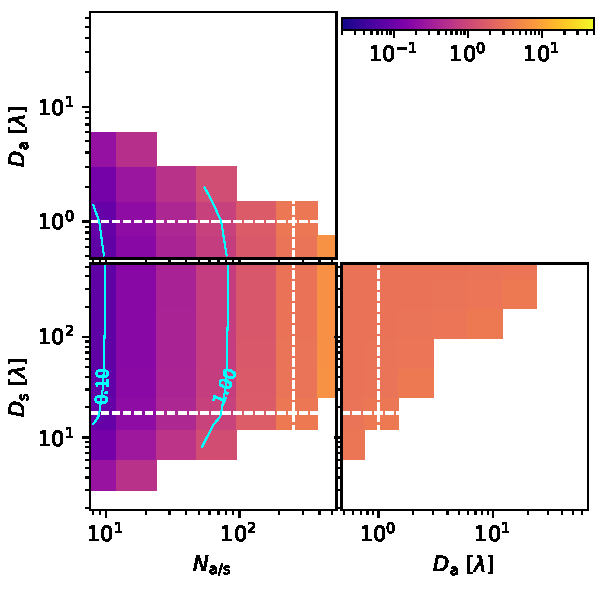
\includegraphics[width=0.48\textwidth]{figures/multidim_xcor_dft_relative_cost_analysis_SKA1-low.pdf}}
% \caption{(Left): Two-dimensional slices of the computational cost for coherent-incoherent imaging using a DFT of station-level cross-correlations for \texttt{SKA-low-core}, \texttt{SKA-low}, \texttt{Aus-VLBA-low}, and \texttt{IC-VLBA-low}. Cyan contours  \label{fig:incoherent-compcost-XBF-SKA-low}}
% \end{figure*}

% \begin{figure}
% 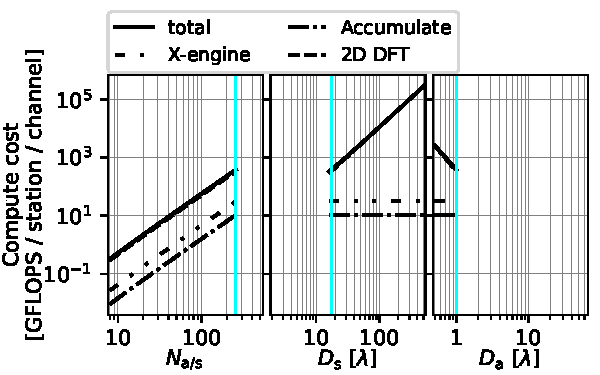
\includegraphics[width=\linewidth]{figures/1D_xcor_dft_cost_analysis_SKA1-low.pdf}
% % 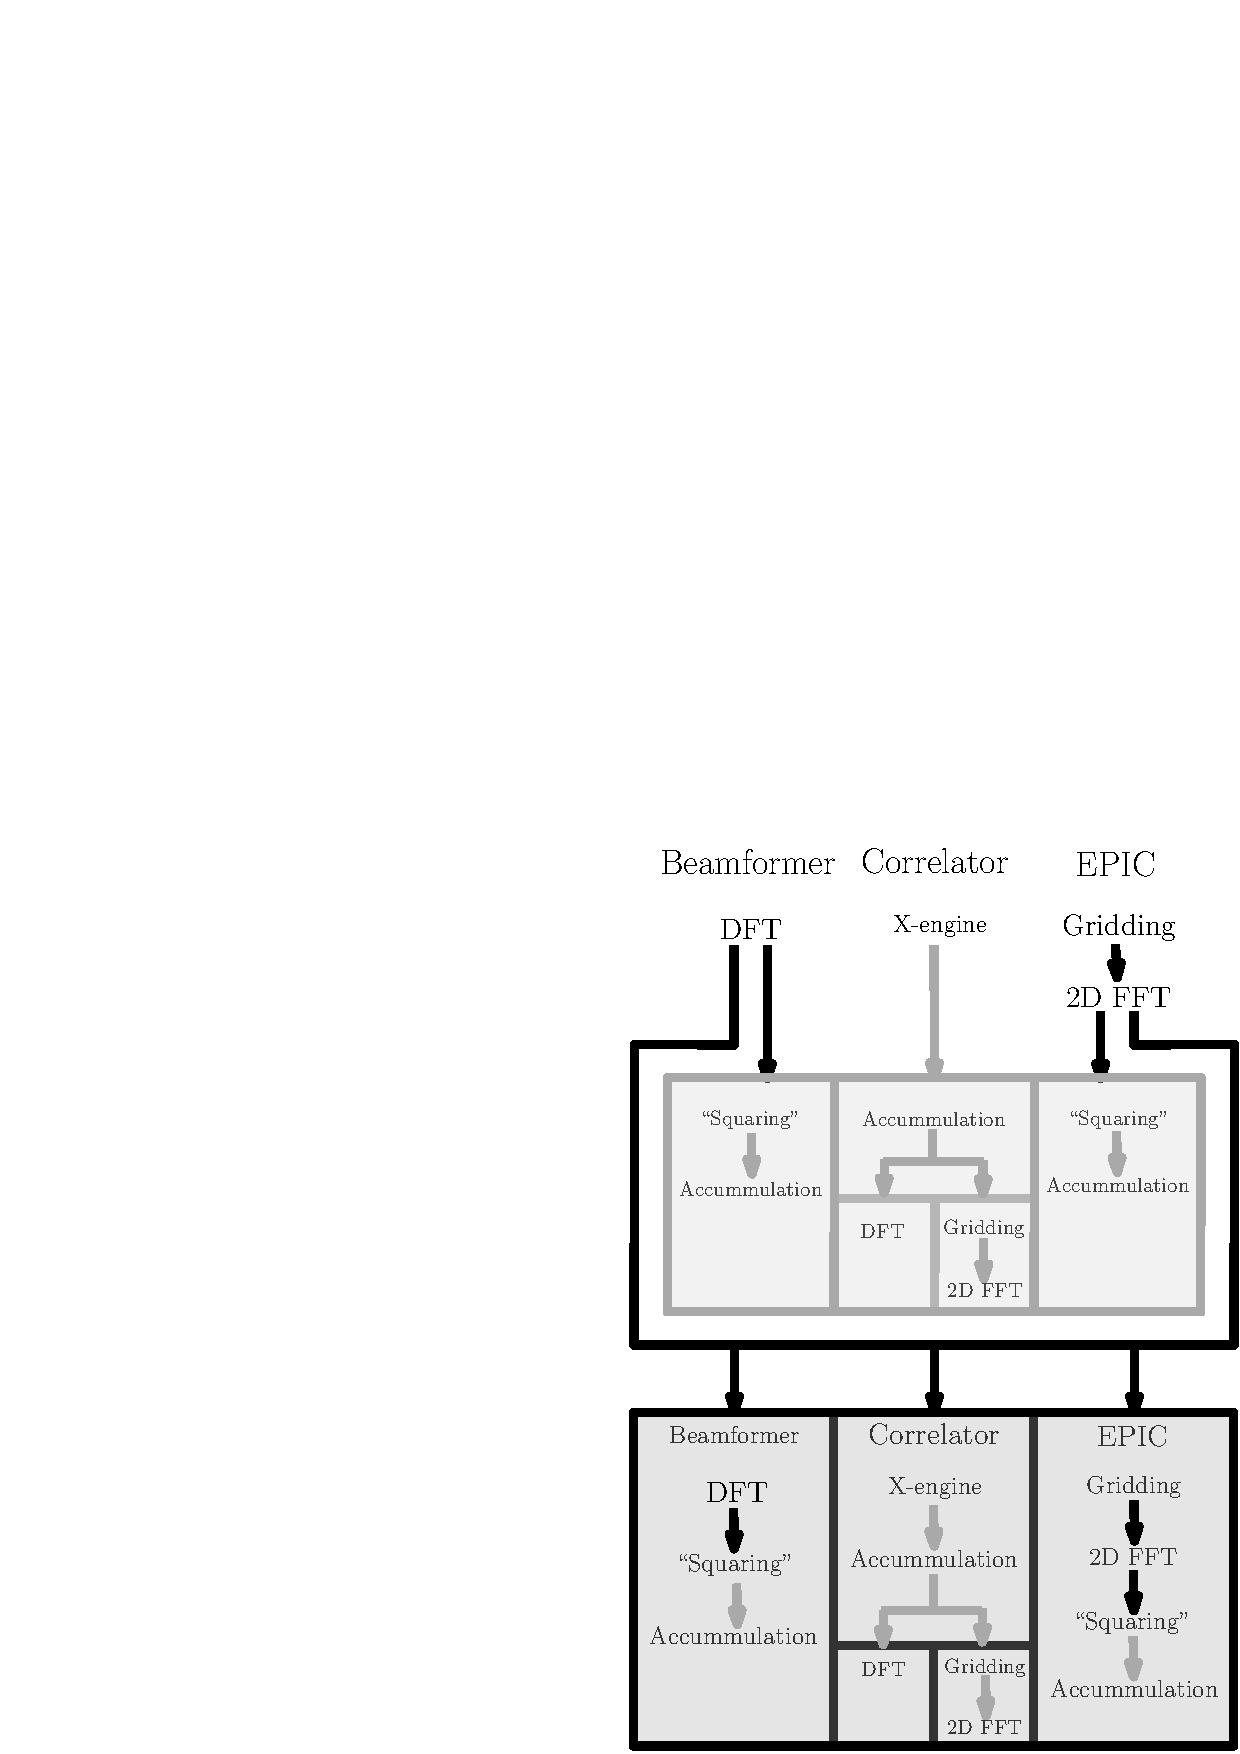
\includegraphics[width=\linewidth]{fig_01.pdf}
% \caption{
% \label{fig:1D-incoherent-compcost-XBF-SKA-low}}
% \end{figure}

% \subsubsection{Correlation and FFT (XFFT)}

\begin{figure}
\includegraphics[width=\linewidth]
% {figures/1D_xcor_fft_cost_analysis_SKA1-low.pdf}
{figures/1D_xcor_fft_per_pixel_cost_analysis_LAMBDA-I.pdf}
\caption{
\label{fig:1D-incoherent-compcost-XFFT-LAMBDA-I}}
\end{figure}

\begin{figure*}
\centering
\subfloat[][Two-dimensional slices \label{fig:multidim-incoherent-compcost-XFFT-LAMBDA-I}]
{\includegraphics[width=0.48\textwidth]
% {figures/multidim_xcor_fft_cost_analysis_SKA1-low.pdf}
{figures/multidim_xcor_fft_per_pixel_cost_analysis_LAMBDA-I.pdf}
}
\subfloat[][Two-dimensional slices (relative)\label{fig:multidim-incoherent-relative-compcost-XFFT-LAMBDA-I}]
{\includegraphics[width=0.48\textwidth]
% {figures/multidim_xcor_fft_relative_cost_analysis_SKA1-low.pdf}
{figures/multidim_xcor_fft_relative_cost_analysis_LAMBDA-I.pdf}
}
\caption{(Left): Two-dimensional slices of the computational cost for coherent-incoherent imaging using an FFT of station-level cross-correlations for . Cyan contours  \label{fig:incoherent-compcost-XFFT-LAMBDA-I}}
\end{figure*}

\begin{figure}
\centering
\subfloat[][One-dimensional slices \label{fig:1D-incoherent-compcost-LAMBDA-I}]
{\includegraphics[width=\textwidth]
% {figures/1D_compcost_analysis_SKA1-low.pdf}
{figures/1D_per_pixel_compcost_analysis_LAMBDA-I.pdf}
} \\
\subfloat[][One-dimensional slices (relative)\label{fig:1D-incoherent-compcost-CASPA}]
{\includegraphics[width=\textwidth]
% {figures/1D_relative_compcost_analysis_SKA1-low.pdf}
{figures/1D_per_pixel_compcost_analysis_CASPA.pdf}
} \\
\subfloat[][One-dimensional slices (relative)\label{fig:1D-incoherent-compcost-FarView}]
{\includegraphics[width=\textwidth]
% {figures/1D_relative_compcost_analysis_SKA1-low.pdf}
{figures/1D_per_pixel_compcost_analysis_FarView.pdf}
}
\caption{(Top): One-dimensional slices of the computational cost for coherent-incoherent imaging using station-level voltage beamforming for \texttt{SKA-low-core}, \texttt{SKA-low}, and \texttt{LAMBDA-I}. (Middle): Same for \texttt{CASPA}. (Bottom): Same for \texttt{FarView}. \label{fig:1D-incoherent-compcost}}
\end{figure}

\section{Inter-station Imaging Architectures} \label{sec:inter-station-arch}

The products from the intra-station architectures form the inputs for inter-station imaging. The intra-station coherent combinations producing $\widetilde{\mathcal{E}}_m^\alpha(\hat{\boldsymbol{s}}_k)$ in Equations~(\ref{eqn:intra-station-pol-hol-img-expl}) and (\ref{eqn:intra-station-pol-hol-img-epic}) effectively act as virtual telescopes measuring the electric fields but simultaneously pointed towards multiple locations, $\hat{\boldsymbol{s}}_k$. Here, we assume that the processing occurs in real time. 

\subsection{Incoherent Architectures} \label{sec:incoherent}

Incoherent inter-station imaging simply involves accumulating the images from each station at a cadence of . The angular resolution remains the same as the intra-station images (assuming all stations have equal angular resolution). This can be achieved through the four methods described in section~\ref{sec:intra-station-arch} by accumulating the intensities, 
\begin{align}
    \widetilde{\mathcal{I}}^{\alpha\beta}(\hat{\boldsymbol{s}}_k) &= \frac{\sum_m w_{km}^{\alpha\beta} \, \widetilde{\mathcal{I}}_m^{\alpha\beta}(\hat{\boldsymbol{s}}_k)}{\sum_m w_{km}^{\alpha\beta}} \, , \label{eqn:inter-station-incoherent-pol-images}
\end{align}
where, $w_{km}^{\alpha\beta}$ represents station weights in the incoherent accumulation of intensities for the intra-station beam centred on $\hat{\boldsymbol{s}}_k$. The incoherent nature of this inter-station intensity accumulation implies that it does not depend on inter-station spacing in the array layout and the array diameter, $D_A$. 

\subsection{Coherent Architectures} \label{sec:coherent}

A coherent combination of data between stations requires electric field data products with phase information from the first stage of processing on individual stations. Thus, intra-station visibilities in which only phase differences remain and from which the original absolute phases have been removed, as well as the image intensity outputs of XBF and XFFT, are unusable for coherent processing at the inter-station level. Hence, we consider two possibilities, namely, the electric fields, $\widetilde{\mathcal{E}}_m^\alpha(\hat{\boldsymbol{s}}_k)$, from VBF and EPIC from equations~\ref{eqn:intra-station-pol-hol-img-expl} and \ref{eqn:intra-station-pol-hol-img-epic-LA}, respectively. 

The pointing direction of the virtual synthesised telescope from the elements of station, $m$ is denoted by $\hat{\boldsymbol{s}}_k$. The field of view and angular resolution of the intra-station $widetilde{\mathcal{E}}_m^\alpha(\hat{\boldsymbol{s}}_k)$ are determined by the station element and the station dimensions, respectively. Using these electric fields as measurements from virtual synthesised telescopes, the inter-station imaging architecture can take any of the architectures that were already discussed under intra-station imaging by combining the electric fields from synthesised telescopes from different stations virtually pointed in the same direction. Since the computational costs depend on the station and array layouts, this necessitates hybrid architectures appropriate for multi-scale aperture arrays. 

Below, $\widetilde{E}_{a_m}^p$ is replaced with the Electric fields, $\widetilde{\mathcal{E}}_m^\alpha(\hat{\boldsymbol{s}}_k)$ (equivalently,  $\widetilde{\boldsymbol{\mathcal{E}}}_{[m,\alpha,\hat{\boldsymbol{s}}]}$) coherently produced by the intra-station processing either through voltage beamforming or EPIC with corresponding changes in replacing intra-station with inter-station terms. We use $\hat{\boldsymbol{\sigma}}_l$ and $\boldsymbol{r}_{m}$ to denote pixel locations within a selected station's resolution solid angle element centred on $\hat{\boldsymbol{s}}_k$, and location of station $m$, respectively. 

\subsubsection{Beamforming}

The inter-station beamforming 
% takes the same form as Equation~(\ref{eqn:intra-station-pol-hol-img-expl}) except $\widetilde{E}_{a_m}^p$ is replaced with beamformed $\widetilde{\mathcal{E}}_m^\alpha(\hat{\boldsymbol{s}}_k)$ and corresponding changes in other terms too. Thus,
can be written as
\begin{align}
    \widetilde{\mathcal{E}}_{\hat{\boldsymbol{s}}_k}^\alpha(\hat{\boldsymbol{\sigma}}_l) &= \sum_{m} \sum_p  \widetilde{\mathcal{W}}_{km}^{{p\alpha}^*}(\hat{\boldsymbol{\sigma}}_l) \, \widetilde{\mathcal{E}}_m^p(\hat{\boldsymbol{s}}_k) \, e^{i\frac{2\pi}{\lambda} \hat{\boldsymbol{\sigma}}_l\cdot\boldsymbol{r}_{m}} \, . \label{eqn:inter-station-pol-hol-img-expl}    
\end{align}
The corresponding polarised intensity at $\hat{\boldsymbol{\sigma}}_l$ within the station resolution element denoted by $\hat{\boldsymbol{s}}_k$, is given by the ``squaring'' and averaging operations, similar to Equation~(\ref{eqn:intra-station-opt-pol-img-outprod}),
\begin{align}
    \widetilde{\mathcal{I}}^{\alpha\beta}_{\hat{\boldsymbol{s}}_k}(\hat{\boldsymbol{\sigma}}_l) &= \left\langle \widetilde{\mathcal{E}}_{\hat{\boldsymbol{s}}_k}^\alpha(\hat{\boldsymbol{\sigma}}_l) \,  \widetilde{\mathcal{E}}_{\hat{\boldsymbol{s}}_k}^{\beta^*}(\hat{\boldsymbol{\sigma}}_l) \right\rangle \, , \label{eqn:inter-station-opt-pol-img-outprod}
\end{align}
where, the angular brackets denote a temporal averaging across an interval of $\Delta t$. The angular resolution of the inter-station beamforming will correspond to the dimensions of the layout of stations within the array.

% The computational budget, $C_\textrm{1VBF+2VBF}$, of coherent inter-station imaging on all independent pixels filling all station resolution elements preceded by intra-station beamforming which fill the entire station field of view can be expressed as
% \begin{align}
%     C_\textrm{1BF+2BF} &= \frac{8 n_\textrm{p}^2}{\delta t} \, \biggl[N_\textrm{a/s} N_\textrm{s}\left(\frac{D_\textrm{s}}{D_\textrm{a}}\right)^2 + N_\textrm{s}\left(\frac{D_\textrm{A}}{D_\textrm{a}}\right)^2 + \left(\frac{D_\textrm{A}}{D_\textrm{a}}\right)^2 \biggr] \, . \label{eqn:cost-1BF-2BF}
% \end{align}
% The first, second, and third terms in the brackets correspond to intra-station voltage beamforming in Equation~(\ref{eqn:intra-station-pol-hol-img-expl}) to produce $\widetilde{E}_{a_m}^p$ on all station resolution elements, inter-station voltage beamforming in Equation~(\ref{eqn:inter-station-pol-hol-img-expl}) on every independent pixel on all station resolution elements, and ``squaring'' and accumulation to obtain intensities in Equation~(\ref{eqn:inter-station-opt-pol-img-outprod}), respectively.  

\subsubsection{EPIC}

% The $\widetilde{E}_{a_m}^p$ produced by intra-station voltage beamforming in Equation~(\ref{eqn:intra-station-pol-hol-img-expl}) forms the input for inter-station EPIC as
% \begin{align}
%     \widetilde{\mathcal{E}}_{\hat{\boldsymbol{s}}_k}^\alpha(\hat{\boldsymbol{\sigma}}_l) &= \sum_j \delta^2 \boldsymbol{r}_j \, e^{i\frac{2\pi}{\lambda} \hat{\boldsymbol{\sigma}}_l\cdot\boldsymbol{r}_j} \left(\sum_{m}\sum_p \widetilde{W}_{m}^{p\alpha*}(\boldsymbol{r}_j-\boldsymbol{r}_{m}) \, \widetilde{\mathcal{E}}_m^p(\hat{\boldsymbol{s}}_k) \right) \, , \label{eqn:inter-station-pol-hol-img-epic}
% \end{align}
% whose equivalent linear algebraic representation is 

Inter-station EPIC takes the form
\begin{align}
    \widetilde{\boldsymbol{\mathcal{E}}}_{[\alpha,\hat{\boldsymbol{\sigma}},\hat{\boldsymbol{s}}]} &= \mathbf{F}^\textrm{H}_{[\hat{\boldsymbol{\sigma}}\leftarrow \boldsymbol{r}]}\,\widetilde{\mathbf{W}}^\textrm{H}_{[\alpha,\boldsymbol{r}\leftarrow p,\boldsymbol{r}_{m}]}\,\widetilde{\boldsymbol{\mathcal{E}}}_{[m,p,\hat{\boldsymbol{s}}]} \, . \label{eqn:inter-station-pol-hol-img-epic-LA}
\end{align}
for producing gridding and two-dimensional FFT electrical fields with an angular resolution corresponding to the full array layout including all stations. The intensities are produced by squaring and accumulation as
\begin{align}
    \widetilde{\mathbf{I}}_{[\alpha\beta,\hat{\boldsymbol{\sigma}},\hat{\boldsymbol{s}}]} &= \left\langle \widetilde{\boldsymbol{\mathcal{E}}}_{[\alpha,\hat{\boldsymbol{\sigma}},\hat{\boldsymbol{s}}]} \bigotimes_{\alpha\beta} \widetilde{\boldsymbol{\mathcal{E}}}_{[\beta,\hat{\boldsymbol{\sigma}},\hat{\boldsymbol{s}}]}^* \right\rangle \, , \label{eqn:inter-station-opt-polarimetric-direct-img-LA}    
\end{align}
where, the outer product is performed over polarisation indices, $\alpha$ and $\beta$, and the the angular brackets denote a temporal averaging across an interval of $\Delta t$.  


\subsubsection{Correlator Beamforming}

The intra-station electric fields, $\widetilde{\boldsymbol{\mathcal{E}}}_{[m,p,\hat{\boldsymbol{s}}]}$ or $\widetilde{\mathcal{E}}_m^p(\hat{\boldsymbol{s}}_k)$, phase-centred towards $\hat{\boldsymbol{s}}_k$ are correlated to produce the inter-station visibilities, 
\begin{align}
    \widetilde{V}_{mn}^{pq}(\hat{\boldsymbol{s}}_k) &= \bigl\langle \widetilde{\mathcal{E}}_m^p(\hat{\boldsymbol{s}}_k) \, \widetilde{\mathcal{E}}_n^{q*}(\hat{\boldsymbol{s}}_k)\bigr\rangle \label{eqn:inter-station-pol-visibilities}
\end{align}
which are then beamformed similar to Equation~(\ref{eqn:intra-station-pol-xbf-img-expl}) to produce the intensities at a higher angular resolution around $\hat{\boldsymbol{s}}_k$ filling the station-scale angular resolution element (equivalently, the array's field of view),
\begin{align}
    \widetilde{\mathcal{I}}^{\alpha\beta}_{\hat{\boldsymbol{s}}_k}(\hat{\boldsymbol{\sigma}}_l)
    &= \sum_{m,n} \sum_{p,q} \widetilde{\mathcal{B}}_{kmn}^{*pq;\alpha\beta}(\hat{\boldsymbol{\sigma}}_l) \, \widetilde{V}_{mn}^{pq}(\hat{\boldsymbol{s}}_k) \,  e^{i\frac{2\pi}{\lambda} \hat{\boldsymbol{\sigma}}_l\cdot\Delta\boldsymbol{r}_{m n}} \, , \label{eqn:inter-station-pol-xbf-img-expl} 
\end{align}
where, $\widetilde{\mathcal{B}}_{kmn}^{*pq;\alpha\beta}(\hat{\boldsymbol{\sigma}}_l)$ is applied to the visibility phase-centred on $\hat{\boldsymbol{s}}_k$ as a directional weighting (direction denoted by $\hat{\boldsymbol{\sigma}}_l$).  

\subsubsection{Correlation FFT}

The visibilities are obtained as in Equation~(\ref{eqn:inter-station-pol-visibilities}) and transformed using an FFT following the same formalism in Equation~(\ref{eqn:intra-station-opt-pol-corr-image}), to yield the polarised intensities,
\begin{align}
    \widetilde{\mathbf{I}}_{[\alpha\beta,\hat{\boldsymbol{\sigma}},\hat{\boldsymbol{s}}]} &= \mathbf{F}^\textrm{H}_{[\hat{\boldsymbol{\sigma}}\leftarrow\Delta\boldsymbol{r}]}\,\widetilde{\mathbf{B}}^\textrm{H}_{[\alpha\beta,\Delta\boldsymbol{r}\leftarrow pq,\Delta\boldsymbol{r}_{mn}]} \mathbf{N}^{-1}_{[mn\leftarrow mn]}\,\widehat{\mathbf{V}}_{[mn,pq,\hat{\boldsymbol{s}}]} \, , \label{eqn:inter-station-opt-pol-corr-image}
\end{align}
where, $\widetilde{\mathbf{B}}^\textrm{H}_{[\alpha\beta,\Delta\boldsymbol{r}\leftarrow pq,\Delta\boldsymbol{r}_{mn}]}$ is the gridding operator that places discrete inverse noise covariance weighted intra-station visibilities onto a array-scale grid and accumulates any visibilities overlapping on the grid points. 

\begin{figure*}
\centering
\subfloat[][\texttt{LAMBDA-I} \label{fig:1D-coherent-compcost-LAMBDA-I}]
{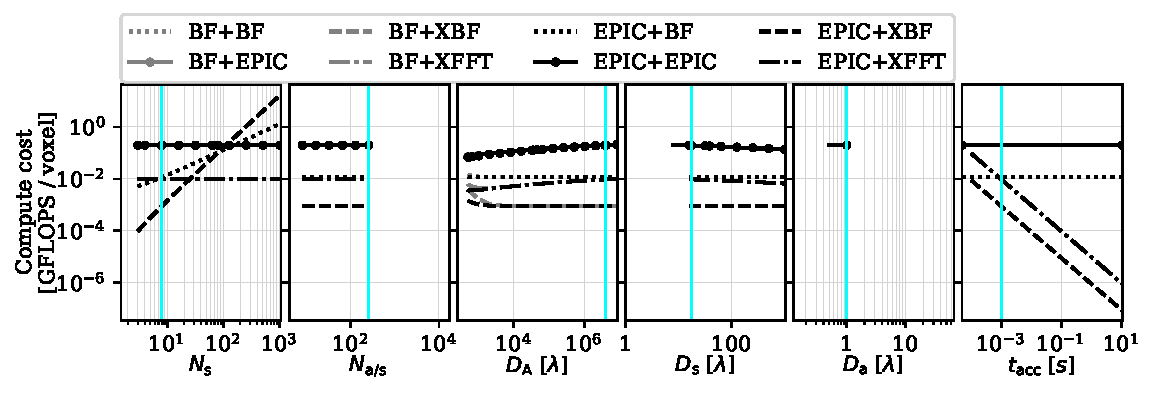
\includegraphics[width=\textwidth]
{figures/1D_coherent_per_pixel_compcost_analysis_LAMBDA-I.pdf}
} \\
\subfloat[][\texttt{SKA1-Low-core} \label{fig:1D-coherent-compcost-LAMBDA-I}]
{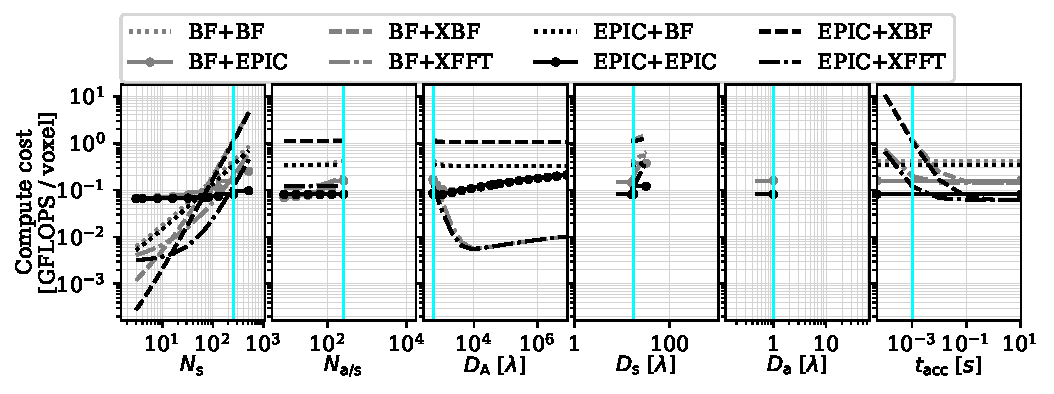
\includegraphics[width=\textwidth]
{figures/1D_coherent_per_pixel_compcost_analysis_SKA1-low-core.pdf}
} \\
\subfloat[][\texttt{SKA1-Low} \label{fig:1D-coherent-compcost-LAMBDA-I}]
{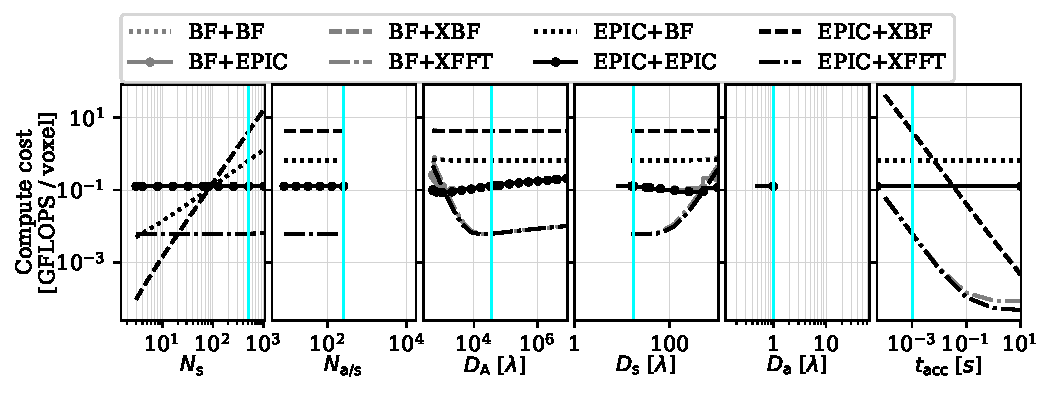
\includegraphics[width=\textwidth]
{figures/1D_coherent_per_pixel_compcost_analysis_SKA1-low.pdf}
} 
\caption{(Top): One-dimensional slices of the computational cost for coherent-incoherent imaging using station-level voltage beamforming for \texttt{SKA-low-core}, \texttt{SKA-low}, and \texttt{LAMBDA-I}. (Middle): Same for \texttt{CASPA}. (Bottom): Same for \texttt{FarView}. \label{fig:1D-incoherent-compcost-a}}
\end{figure*}

\begin{figure*}\ContinuedFloat
\subfloat[][\texttt{CASPA} \label{fig:1D-coherent-compcost-CASPA}]
{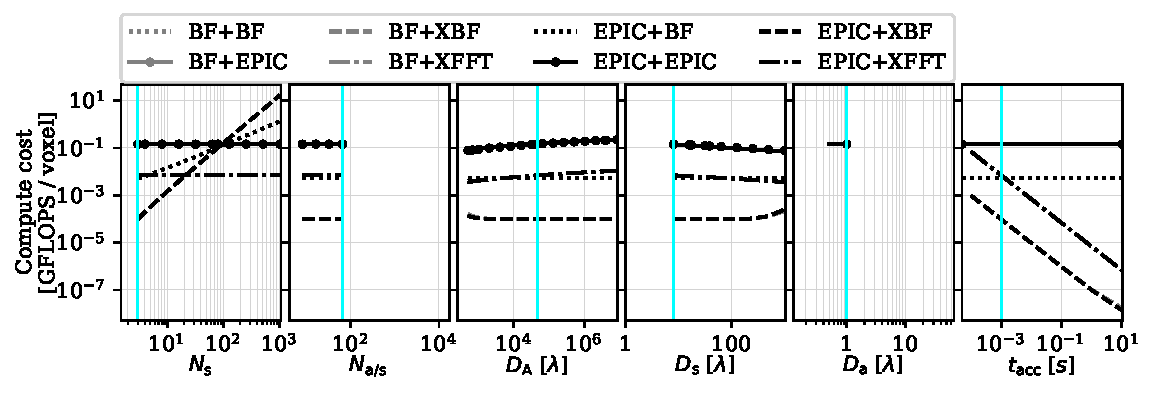
\includegraphics[width=\textwidth]
{figures/1D_coherent_per_pixel_compcost_analysis_CASPA.pdf}
} \\
\subfloat[][\texttt{FarView} \label{fig:1D-coherent-compcost-FarView}]
{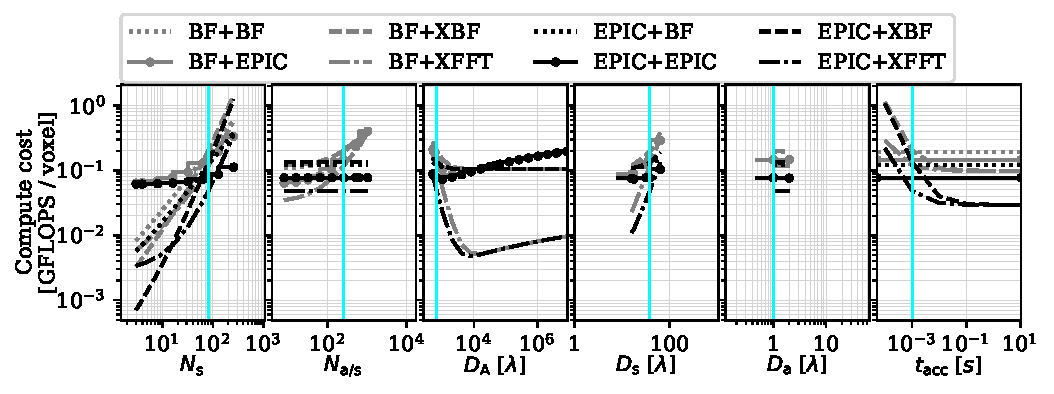
\includegraphics[width=\textwidth]
{figures/1D_coherent_per_pixel_compcost_analysis_FarView.pdf}
}
\caption{Contd. (Top): One-dimensional slices of the computational cost for coherent-incoherent imaging using station-level voltage beamforming for \texttt{SKA-low-core}, \texttt{SKA-low}, and \texttt{LAMBDA-I}. (Middle): Same for \texttt{CASPA}. (Bottom): Same for \texttt{FarView}. \label{fig:1D-incoherent-compcost}}
\end{figure*}

\begin{table*}[htb!]
\normalsize
\begin{threeparttable}
\caption{Computational budget of intra- and inter-station coherent imaging architectures.}
\label{tab:intra-inter-station-coherent-imaging}
% \begin{tabularx}{\textwidth}{ccccc}
\begin{tabular}{ccccc}
\toprule
\headrow Architecture & Components & Intra-station & Inter-station & Equations \\
 & (Timescale) & FLOP count & FLOP count & \\ 
 & & (per station & (per station beam  & \\
 & & per channel) & per channel) & \\
\midrule\midrule
VBF & Beamforming ($\delta t$) & $8 n_\textrm{p}^2 N_\textrm{a/s} \left(\frac{D_\textrm{s}}{D_\textrm{a}}\right)^2$ & $8 n_\textrm{p}^2 N_\textrm{s}\left(\frac{D_\textrm{A}}{D_\textrm{s}}\right)^2$ & \ref{eqn:intra-station-pol-hol-img-expl}, \ref{eqn:inter-station-pol-hol-img-expl} \\
& Squaring ($\delta t$) & $6 n_\textrm{p}^2 \left(\frac{D_\textrm{s}}{D_\textrm{a}}\right)^2$ & $6 n_\textrm{p}^2 \left(\frac{D_\textrm{A}}{D_\textrm{s}}\right)^2$ & \ref{eqn:intra-station-opt-pol-img-outprod} , \ref{eqn:inter-station-opt-pol-img-outprod}  \\
& Accumulation ($\delta t$ ) & $2 n_\textrm{p}^2 \left(\frac{D_\textrm{s}}{D_\textrm{a}}\right)^2$ & $2 n_\textrm{p}^2 \left(\frac{D_\textrm{A}}{D_\textrm{s}}\right)^2$ & \ref{eqn:intra-station-opt-pol-img-outprod}, \ref{eqn:inter-station-opt-pol-img-outprod} \\
\midrule
EPIC & Gridding ($\delta t$) & $6 n_\textrm{p}^2 N_\textrm{a/s} N_\textrm{ka}$ & $6 n_\textrm{p}^2 N_\textrm{s} N_\textrm{ks}$ & \ref{eqn:intra-station-pol-hol-img-epic-LA}, \ref{eqn:inter-station-pol-hol-img-epic-LA}   \\
& FFT ($\delta t$) & $8 n_\textrm{p} \frac{r}{\log_2 r} \left(\gamma_\textrm{s}\frac{D_\textrm{s}}{D_\textrm{a}}\right)^2\log_2\left(\gamma_\textrm{s}\frac{D_\textrm{s}}{D_\textrm{a}}\right)^2$ & $8 n_\textrm{p} \frac{r}{\log_2 r} \left(\gamma_\textrm{A}\frac{D_\textrm{A}}{D_\textrm{S}}\right)^2\log_2\left(\gamma_\textrm{A}\frac{D_\textrm{A}}{D_\textrm{S}}\right)^2$ & \ref{eqn:intra-station-pol-hol-img-epic-LA}, \ref{eqn:inter-station-pol-hol-img-epic-LA} \\
& Squaring ($\delta t$) & $6 n_\textrm{p}^2 \left(\gamma_\textrm{s} \frac{D_\textrm{s}}{D_\textrm{a}}\right)^2$ & $6 n_\textrm{p}^2 \left(\gamma_\textrm{A} \frac{D_\textrm{A}}{D_\textrm{s}}\right)^2$ & \ref{eqn:intra-station-opt-polarimetric-direct-img-LA}, \ref{eqn:inter-station-opt-polarimetric-direct-img-LA} \\
& Accumulation ($\delta t$) & $2 n_\textrm{p}^2 \left(\gamma_\textrm{s} \frac{D_\textrm{s}}{D_\textrm{a}}\right)^2$ & $2 n_\textrm{p}^2 \left(\gamma_\textrm{A} \frac{D_\textrm{A}}{D_\textrm{s}}\right)^2$ & \ref{eqn:intra-station-opt-polarimetric-direct-img-LA}, \ref{eqn:inter-station-opt-polarimetric-direct-img-LA} \\
\midrule
XBF & Correlator ($\delta t$) & $6 n_\textrm{p}^2 N_\textrm{a/s} (N_\textrm{a/s}-1)/2$ & $6 n_\textrm{p}^2 N_\textrm{s} (N_\textrm{s}-1)/2$ & \ref{eqn:intra-station-pol-visibilities}, \ref{eqn:inter-station-pol-visibilities}  \\
& Accumulation ($\delta t$) & $2 n_\textrm{p}^2 N_\textrm{a/s} (N_\textrm{a/s}-1)/2$ & $2 n_\textrm{p}^2  N_\textrm{s} (N_\textrm{s}-1)/2$ & \ref{eqn:intra-station-pol-visibilities}, \ref{eqn:inter-station-pol-visibilities}  \\
& DFT ($\Delta t$) & $8 n_\textrm{p}^2 \left(\frac{D_\textrm{s}}{D_\textrm{a}}\right)^2 N_\textrm{a/s} (N_\textrm{a/s}-1)/2$ & $8 n_\textrm{p}^2 \left(\frac{D_\textrm{A}}{D_\textrm{s}}\right)^2 N_\textrm{s} (N_\textrm{s}-1)/2$ & \ref{eqn:intra-station-pol-xbf-img-expl}, \ref{eqn:inter-station-pol-xbf-img-expl}  \\
\midrule
XFFT & Correlator ($\delta t$) & $6 n_\textrm{p}^2 N_\textrm{a/s} (N_\textrm{a/s}-1)/2$ & $6 n_\textrm{p}^2 N_\textrm{s} (N_\textrm{s}-1)/2$ & \ref{eqn:intra-station-pol-visibilities}, \ref{eqn:inter-station-pol-visibilities}  \\
& Accumulation ($\delta t$) & $2 n_\textrm{p}^2 N_\textrm{a/s} (N_\textrm{a/s}-1)/2$ & $2 n_\textrm{p}^2 N_\textrm{s} (N_\textrm{s}-1)/2$ & \ref{eqn:intra-station-pol-visibilities}, \ref{eqn:inter-station-pol-visibilities} \\
& Gridding ($\Delta t$) & 8$n_\textrm{p}^4 (2^2 N_\textrm{ka}) N_\textrm{a/s} (N_\textrm{a/s}-1)/2$ & $8 n_\textrm{p}^4 (2^2 N_\textrm{ks}) N_\textrm{s} (N_\textrm{s}-1)/2$ & \ref{eqn:intra-station-opt-pol-corr-image}, \ref{eqn:inter-station-opt-pol-corr-image} \\
& FFT ($\Delta t$) & $8 n_\textrm{p}^2 \frac{r}{\log_2 r} \left(\frac{D_\textrm{s}}{D_\textrm{a}}\right)^2\log_2\left(\frac{D_\textrm{s}}{D_\textrm{a}}\right)^2$ & $8 n_\textrm{p}^2 \frac{r}{\log_2 r} \left(\frac{D_\textrm{A}}{D_\textrm{S}}\right)^2\log_2\left(\frac{D_\textrm{A}}{D_\textrm{S}}\right)^2$ & \ref{eqn:intra-station-opt-pol-corr-image}, \ref{eqn:inter-station-opt-pol-corr-image} \\
% \midrule
% Three & Four&three three\tnote{b} &four & & \\
\bottomrule
% \end{tabularx}
\end{tabular}
\begin{tablenotes}[hang]
% \item[]Table note
\item[a]Array filling factor, $\,f_\textrm{A}=N_\textrm{s}\,(D_\textrm{s}/D_\textrm{A})^2$
% \item[b]Station filling factor, $\,f_\textrm{s}=N_\textrm{a/s}\,(D_\textrm{a}/D_\textrm{s})^2$
\end{tablenotes}
\end{threeparttable}
\end{table*}


% \begin{table*}[htb!]
% \normalsize
% \begin{threeparttable}
% \caption{Computational budget of inter-station coherent imaging architectures}
% \label{tab:inter-station-coherent-imaging}
% % \begin{tabularx}{\textwidth}{ccccc}
% \begin{tabular}{ccccc}
% \toprule
% \headrow Inter-station & Components & Equation & FLOP count & Timescale \\
% architecture & & & (per channel) & \\ 
% \midrule\midrule
% VBF & Beamforming & \ref{eqn:inter-station-pol-hol-img-expl} & $8 n_\textrm{p}^2 N_\textrm{s}\left(\frac{D_\textrm{A}}{D_\textrm{s}}\right)^2\left(\frac{D_\textrm{s}}{D_\textrm{a}}\right)^2$ & $\delta t$ \\
% & Squaring & \ref{eqn:inter-station-opt-pol-img-outprod} & $6 n_\textrm{p}^2 \left(\frac{D_\textrm{A}}{D_\textrm{s}}\right)^2\left(\frac{D_\textrm{s}}{D_\textrm{a}}\right)^2$ & $\delta t$ \\
% & Accumulation & \ref{eqn:inter-station-opt-pol-img-outprod} & $2 n_\textrm{p}^2 \left(\frac{D_\textrm{A}}{D_\textrm{s}}\right)^2\left(\frac{D_\textrm{s}}{D_\textrm{a}}\right)^2$ & $\delta t$ \\
% \midrule
% EPIC & Gridding & \ref{eqn:inter-station-pol-hol-img-epic-LA} & $6 n_\textrm{p}^2 N_\textrm{s} N_\textrm{ks}$ & $\delta t$ \\
% & FFT & \ref{eqn:inter-station-pol-hol-img-epic-LA} & $8 n_\textrm{p} \frac{r}{\log_2 r} \left(\gamma_\textrm{A}\frac{D_\textrm{A}}{D_\textrm{S}}\right)^2\log_2\left(\gamma_\textrm{A}\frac{D_\textrm{A}}{D_\textrm{S}}\right)^2$ & $\delta t$ \\
% & Squaring & \ref{eqn:inter-station-opt-polarimetric-direct-img-LA} & $6 n_\textrm{p}^2 \left(\gamma_\textrm{A} \frac{D_\textrm{A}}{D_\textrm{s}}\right)^2\left(\frac{D_\textrm{s}}{D_\textrm{a}}\right)^2$ & $\delta t$ \\
% & Accumulation & \ref{eqn:inter-station-opt-polarimetric-direct-img-LA} & $2 n_\textrm{p}^2 \left(\gamma_\textrm{A} \frac{D_\textrm{A}}{D_\textrm{s}}\right)^2\left(\frac{D_\textrm{s}}{D_\textrm{a}}\right)^2$ & $\delta t$ \\
% \midrule
% XBF & Correlator & \ref{eqn:inter-station-pol-visibilities} & $6 n_\textrm{p}^2 \left(\frac{D_\textrm{s}}{D_\textrm{a}}\right)^2 N_\textrm{s} (N_\textrm{s}-1)/2$ & $\delta t$ \\
% & Accumulation & \ref{eqn:inter-station-pol-visibilities} & $2 n_\textrm{p}^2 \left(\frac{D_\textrm{s}}{D_\textrm{a}}\right)^2 N_\textrm{s} (N_\textrm{s}-1)/2$ & $\delta t$ \\
% & DFT & \ref{eqn:inter-station-pol-xbf-img-expl} & $8 n_\textrm{p}^2 \left(\frac{D_\textrm{A}}{D_\textrm{s}}\right)^2 \left(\frac{D_\textrm{s}}{D_\textrm{a}}\right)^2 N_\textrm{s} (N_\textrm{s}-1)/2$ & $\Delta t$ \\
% \midrule
% XFFT & Correlator & \ref{eqn:inter-station-pol-visibilities} & $6 n_\textrm{p}^2 \left(\frac{D_\textrm{s}}{D_\textrm{a}}\right)^2 N_\textrm{s} (N_\textrm{s}-1)/2$ & $\delta t$ \\
% & Accumulation & \ref{eqn:inter-station-pol-visibilities} & $2 n_\textrm{p}^2 \left(\frac{D_\textrm{s}}{D_\textrm{a}}\right)^2 N_\textrm{s} (N_\textrm{s}-1)/2$ & $\delta t$ \\
% & Gridding & \ref{eqn:inter-station-opt-pol-corr-image} & $8 n_\textrm{p}^4 \left(\frac{D_\textrm{s}}{D_\textrm{a}}\right)^2 (2^2 N_\textrm{ks}) N_\textrm{s} (N_\textrm{s}-1)/2$ & $\Delta t$ \\
% & FFT & \ref{eqn:inter-station-opt-pol-corr-image} & $8 n_\textrm{p}^2 \frac{r}{\log_2 r} \left(\frac{D_\textrm{s}}{D_\textrm{a}}\right)^2 \left(\frac{D_\textrm{A}}{D_\textrm{S}}\right)^2\log_2\left(\frac{D_\textrm{A}}{D_\textrm{S}}\right)^2$ & $\Delta t$ \\
% % \midrule
% % Three & Four&three three\tnote{b} &four & & \\
% \bottomrule
% % \end{tabularx}
% \end{tabular}
% \begin{tablenotes}[hang]
% % \item[]Table note
% \item[a]Array filling factor, $\,f_\textrm{A}=N_\textrm{s}\,(D_\textrm{s}/D_\textrm{A})^2$
% % \item[b]Station filling factor, $\,f_\textrm{s}=N_\textrm{a/s}\,(D_\textrm{a}/D_\textrm{s})^2$
% \end{tablenotes}
% \end{threeparttable}
% \end{table*}

% \subsection{Stage I: Intra-station Architectures} \label{sec:intra-station-arch}

% We first describe the first stage, namely, intra-station architectures that form the basis for both approaches. This first stage essentially synthesises station-scale apertures with simultaneous, multiple virtual pointings. These station-scale apertures from the first stage will act as fundamental elements for the second stage of inter-station processing. We will use $a_m$ to denote element, $a$, in station, $m$.

% \subsubsection{Voltage Beamforming (BF)}

% The calibrated electric fields recorded by individual elements within a station can be phase-coherently superposed towards any desired direction as
% \begin{align}
%     \widetilde{\mathcal{E}}_m^\alpha(\hat{\boldsymbol{s}}_k) &= \sum_{a_m} \sum_p  \widetilde{\mathcal{W}}_{a_m}^{{p\alpha}^*}(\hat{\boldsymbol{s}}_k) \, \widetilde{E}_{a_m}^p \, e^{i\frac{2\pi}{\lambda} \hat{\boldsymbol{s}}_k\cdot\boldsymbol{r}_{a_m}} \, , \label{eqn:pol-hol-img-expl}
% \end{align}
% where, $\hat{\boldsymbol{s}}_k$ denotes the direction of beam, $k$, towards which the measurements are phase-coherently superposed, $\widetilde{E}_{a_m}^{p}$ represents the calibrated and potentially noise-weighted electric field measured by the station element $a_m$, and $\widetilde{\mathcal{W}}_{a_m}^{{p\alpha}^*}(\hat{\boldsymbol{s}}_k)$ denotes a complex-valued directional weighting\footnote{One can choose $\widetilde{\mathcal{W}}_{a_m}^{p\alpha}(\hat{\boldsymbol{s}}_k)=\mathcal{W}_{a_m}^{p\alpha}(\hat{\boldsymbol{s}}_k)$, the directional electric field sensitivity, if the signal-to-noise ratio is to be optimised. But it can also be generically chosen depending on the property desired of the estimator \cite[][]{Morales2011}.} applied to the station element. This beamforming step has to be executed at a cadence of $\delta t$. 

% The polarised intensity in a pixel is then obtained by
% \begin{align}
%     \widetilde{\mathcal{I}}^{\alpha\beta}_m(\hat{\boldsymbol{s}}_k) &= \left\langle \widetilde{\mathcal{E}}_m^\alpha(\hat{\boldsymbol{s}}_k) \,  \widetilde{\mathcal{E}}_m^{\beta^*}(\hat{\boldsymbol{s}}_k) \right\rangle \, , \label{eqn:opt-pol-img-outprod}
% \end{align}
% where, the angular brackets denote a temporal averaging across an interval of $\Delta t$. Even though it is an outer product over the polarisation axis, we will refer to it as a ``squaring'' operation hereafter for convenience because of what it reduces to if only a single polarisation was measured. 

% The solid angle of the beamformed pixel using the intra-station data is given by $\Omega_s \simeq (\lambda/D_\textrm{s})^2$. Beamforming can be applied to all independent beams ($n_\textrm{bs}$) filling the field of view, whose solid angle is $\Omega_a \simeq (\lambda/D_\textrm{a})^2$. Thus, $n_\textrm{bs} \simeq \Omega_\textrm{a}/\Omega_\textrm{s}=(D_\textrm{s}/D_\textrm{a})^2$. 

% The computational cost budget consists of the following components. Beamforming $N_\textrm{a/s}$ element polarised voltages (with $n_\textrm{p}$ polarisations) towards $n_\textrm{bs}$ beams on sky as per Equation~(\ref{eqn:pol-hol-img-expl}) requires $n_\textrm{p} n_\textrm{bs} N_\textrm{a/s}$ CMACs to get one polarised voltage on sky per station per channel. To get $n_\textrm{p}$ polarised voltages from beamforming, it requires $n_\textrm{p}^2 n_\textrm{bs} N_\textrm{a/s}$ CMACs amounting to $8 n_\textrm{p}^2 n_\textrm{bs} N_\textrm{a/s}/\delta t$ FLOPS per station per channel. 

% Converting polarised beamformed voltages on the sky to Stokes intensities and temporally averaging them as per Equation~(\ref{eqn:opt-pol-corr-img-outprod}) requires $n_\textrm{p}^2$ complex "squaring" (complex products) and subsequent complex additions for each of the complex polarised intensity beams, and therefore $n_\textrm{p}^2 n_\textrm{bs}$ CMACs per station per channel, amounting to $8 n_\textrm{p}^2 n_\textrm{bs}$ FLOPS per station per channel. Hence, the net rate corresponding to beamforming, squaring, and averaging is
% \begin{align}
%     C_\textrm{VBF} &= 8 n_\textrm{p}^2 \, \left(\frac{D_\textrm{s}}{D_\textrm{a}}\right)^2 \, (N_\textrm{a/s}+1) \, \frac{1}{\delta t} \, . \label{eqn:cost-VBF}
% \end{align}


% % \begin{figure*}
% % \centering
% % \subfloat[][Two-dimensional slices \label{fig:multidim-incoherent-compcost-BF-SKA-low}]{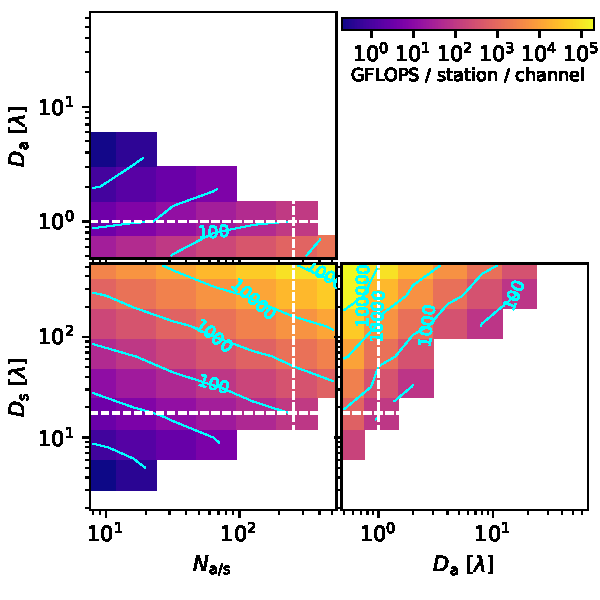
\includegraphics[width=0.4\textwidth]{figures/multidim_beamformer_dft_cost_analysis_SKA1-low.pdf}}
% % \subfloat[][One-dimensional slices\label{fig:1D-incoherent-compcost-BF-SKA-low}]{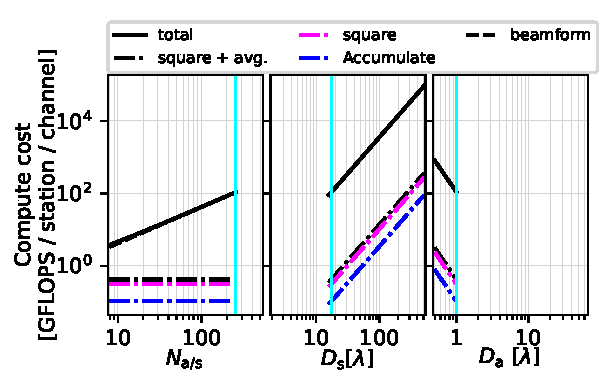
\includegraphics[width=0.58\textwidth]{figures/1D_beamformer_dft_cost_analysis_SKA1-low.pdf}}
% % \caption{(Left): Two-dimensional slices of the computational cost for coherent-incoherent imaging using station-level voltage beamforming for \texttt{SKA-low-core}, \texttt{SKA-low}, \texttt{Aus-VLBA-low}, and \texttt{IC-VLBA-low}. Cyan contours  \label{fig:incoherent-compcost-BF-SKA-low}}
% % \end{figure*}

% \begin{figure}
% 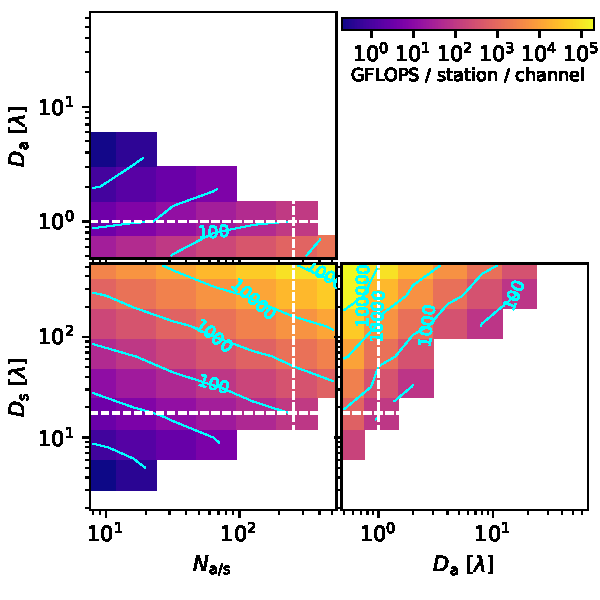
\includegraphics[width=\linewidth]{figures/multidim_beamformer_dft_cost_analysis_SKA1-low.pdf}
% % 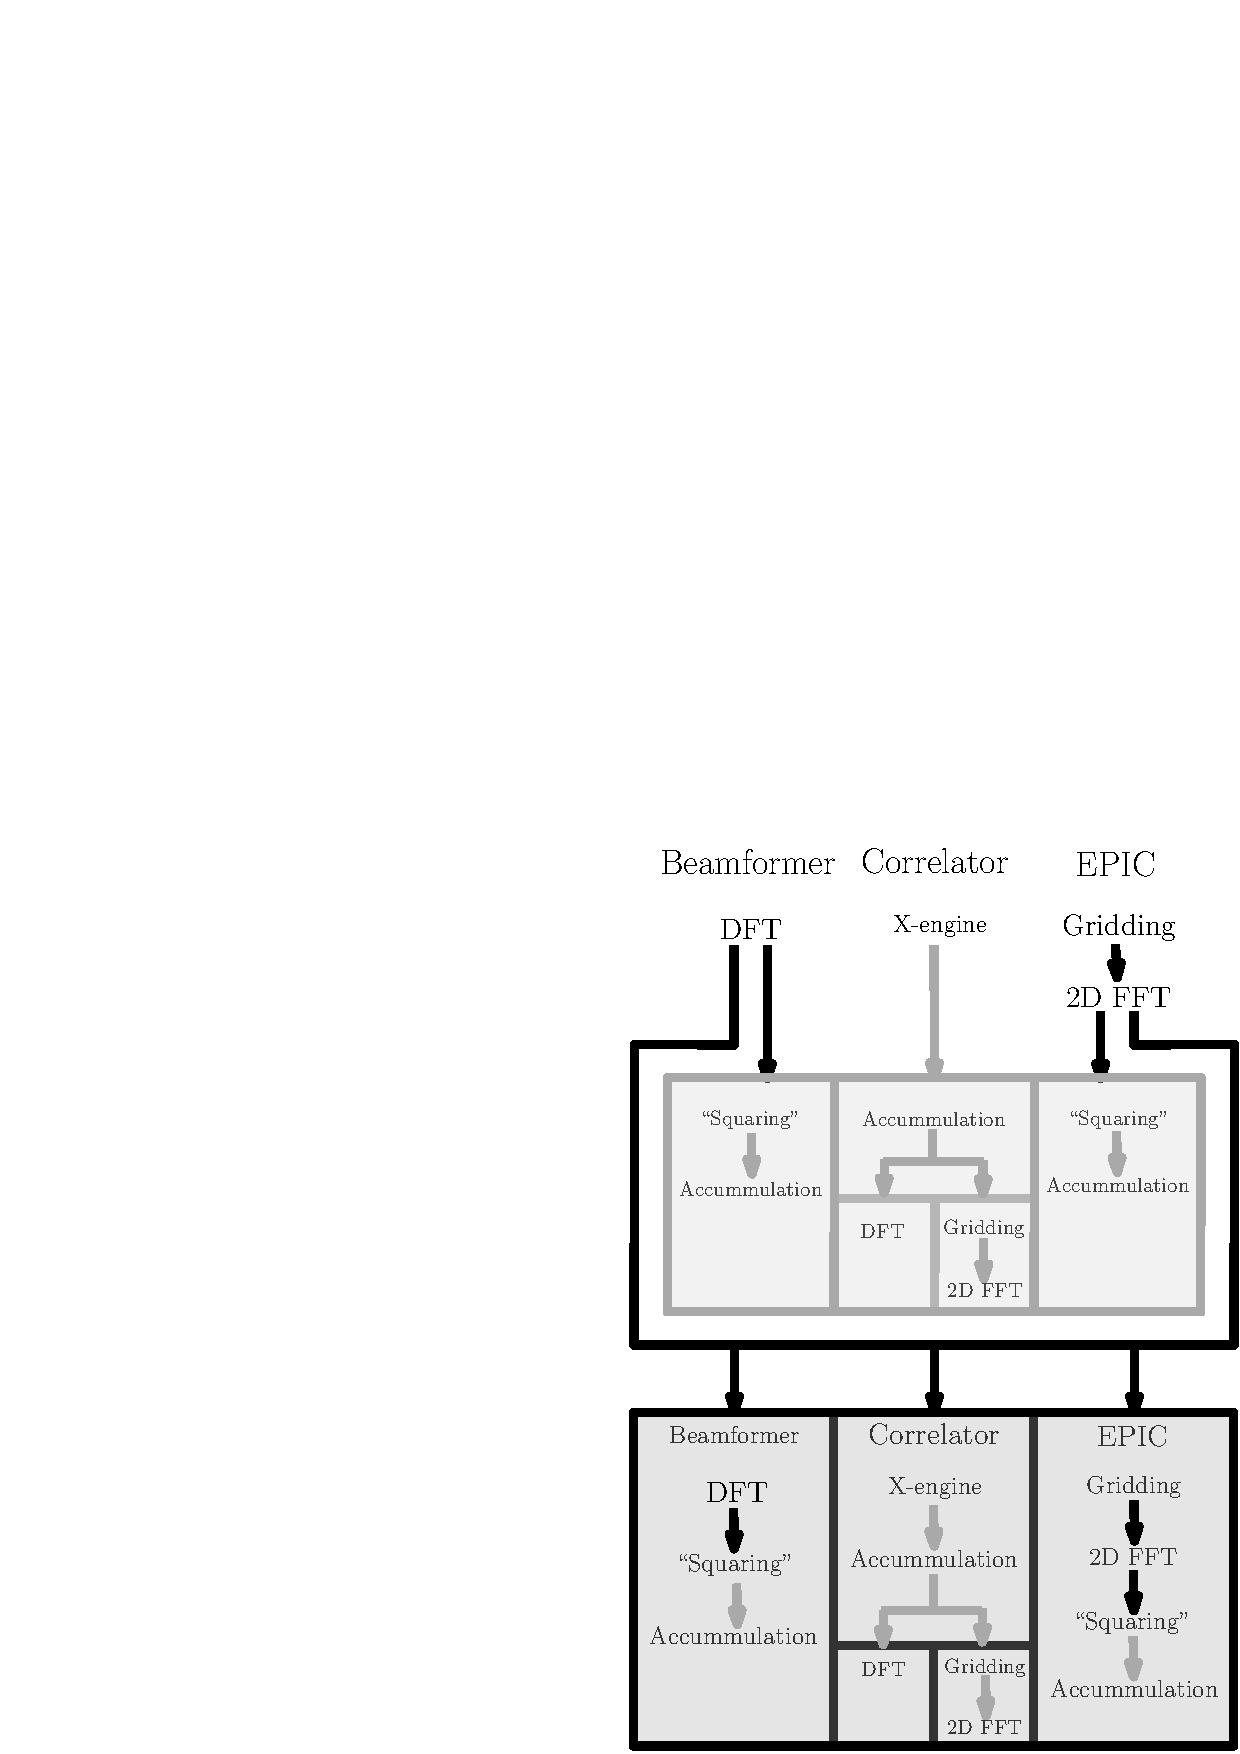
\includegraphics[width=\linewidth]{fig_01.pdf}
% \caption{
% \label{fig:multidim-incoherent-compcost-BF-SKA-low}}
% \end{figure}

% \begin{figure}
% 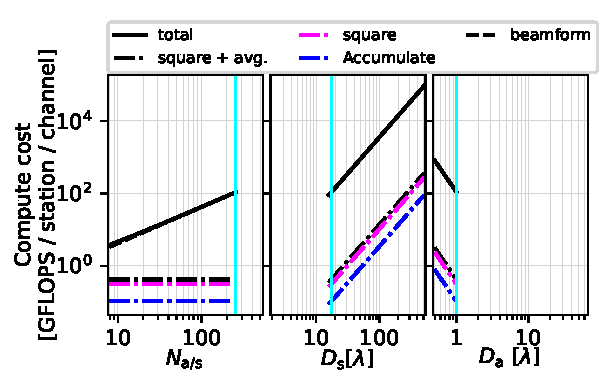
\includegraphics[width=\linewidth]{figures/1D_beamformer_dft_cost_analysis_SKA1-low.pdf}
% % 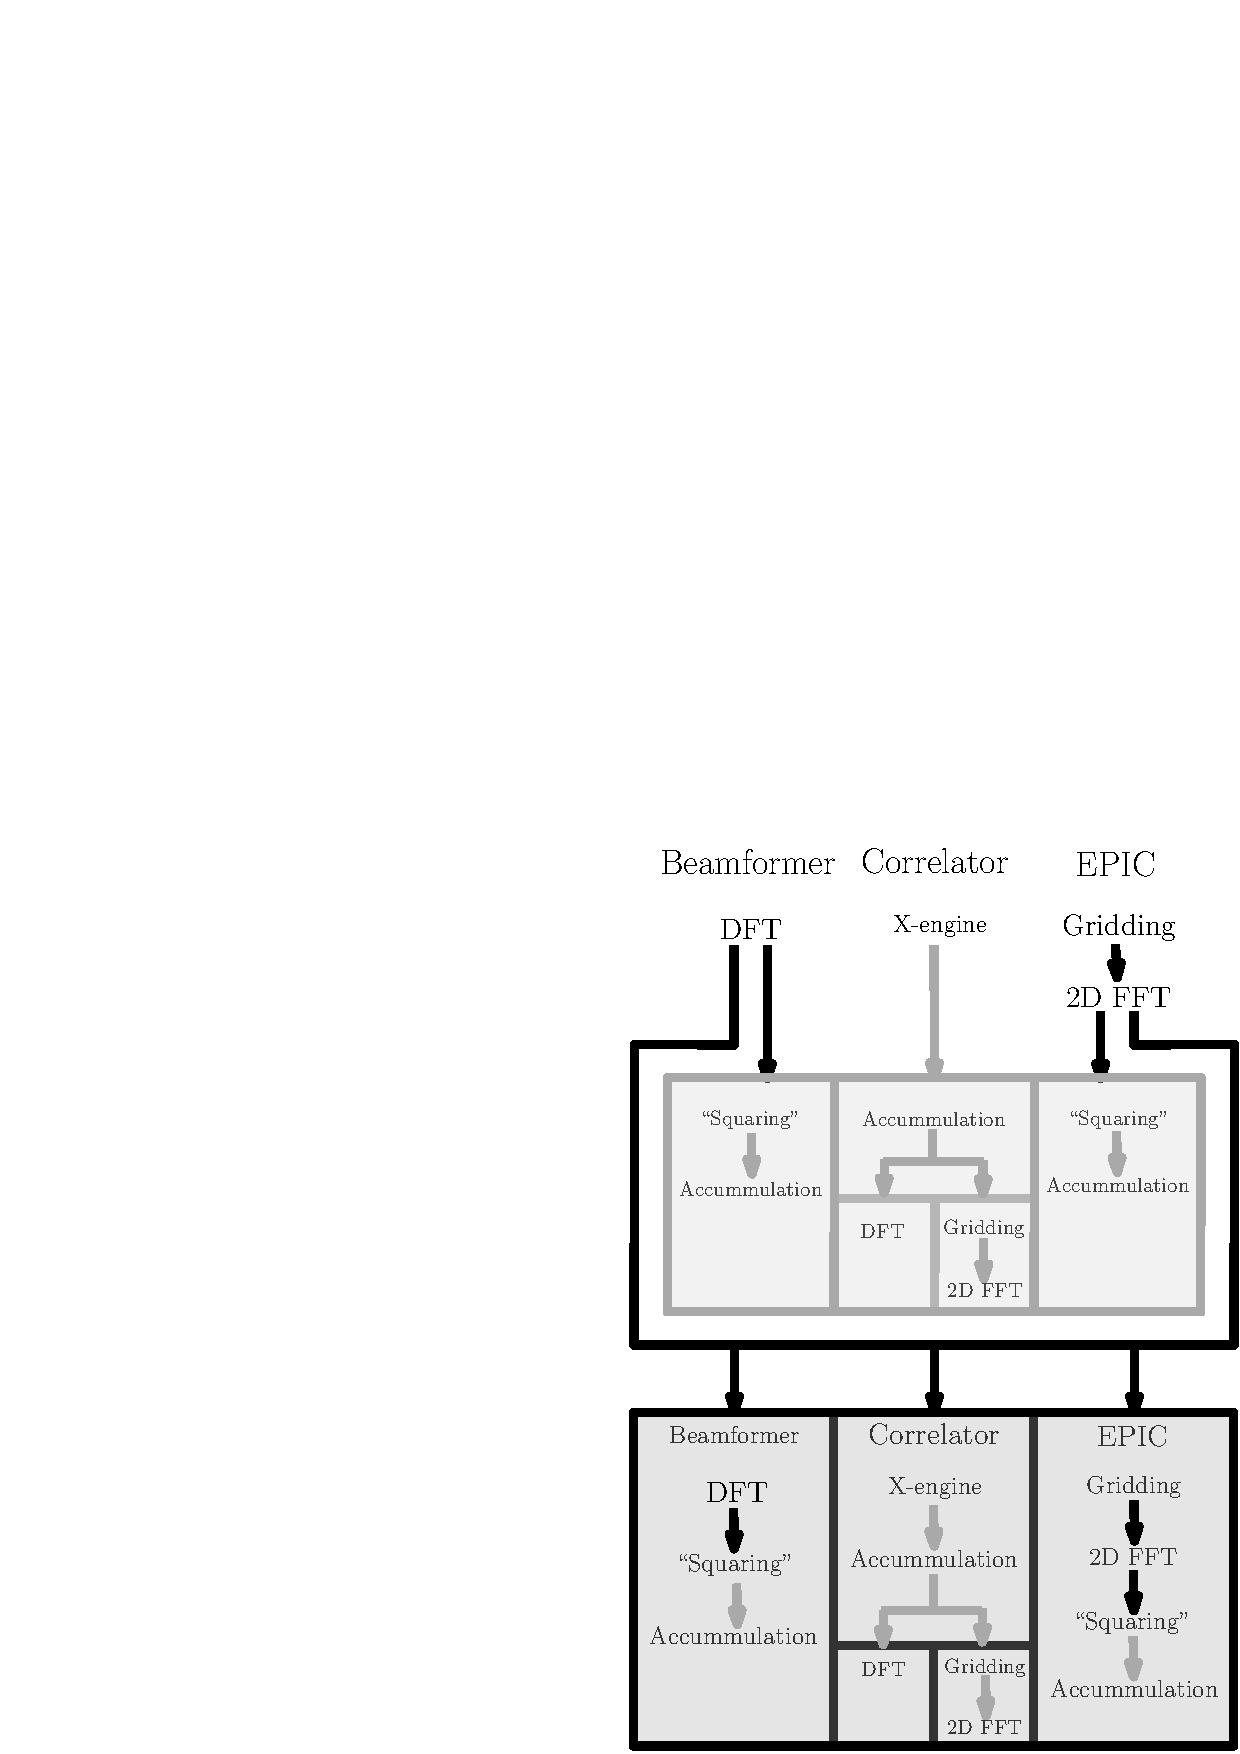
\includegraphics[width=\linewidth]{fig_01.pdf}
% \caption{
% \label{fig:1D-incoherent-compcost-BF-SKA-low}}
% \end{figure}

% \subsubsection{E-field Parallel Imaging Correlator (EPIC)}

% A simultaneous beamforming filling the entire field of view can also be achieved by a two-dimensional spatial Fast Fourier Transform (FFT) of the pre-correlation voltage measurements on the aperture plane. This can be enabled even for an irregular layout of station elements by gridding the calibrated electric fields measured by the station elements. The formalism in \citet{Morales2011} is the basis of the architecture called E-field Parallel Imaging Correlator \citep[EPIC;][]{Thyagarajan+2017,Beardsley+2017}, which has been implemented on the LWA station in Sevilleta (NM, USA) using GPU \citep{Kent+2019,Kent+2020,Krishnan+2023}. 

% The polarised electric fields on the sky can be reconstructed from the calibrated electric fields measured by the antennas as 
% \begin{align}
%     \widetilde{\mathcal{E}}_m^\alpha(\hat{\boldsymbol{s}}_k) &= \sum_j \delta^2 \boldsymbol{r}_j \, e^{i\frac{2\pi}{\lambda} \hat{\boldsymbol{s}}_k\cdot\boldsymbol{r}_j} \left(\sum_{a_m} \widetilde{W}_{a_m}^{p\alpha*}(\boldsymbol{r}_j-\boldsymbol{r}_{a_m}) \, \widetilde{E}_{a_m}^p \right) \, , \label{eqn:pol-hol-img}
% \end{align}
% whose equivalent linear algebraic representation is 
% \begin{align}
%     \widetilde{\boldsymbol{\mathcal{E}}}_{[m,\alpha,\hat{\boldsymbol{s}}]} &= \mathbf{F}^\textrm{H}_{[\hat{\boldsymbol{s}}\leftarrow \boldsymbol{r}]}\,\widetilde{\mathbf{W}}^\textrm{H}_{[\alpha,\boldsymbol{r}\leftarrow p,\boldsymbol{r}_{a_m}]}\,\widetilde{\mathbf{E}}_{[p,\boldsymbol{r}_{a_m}]} \, . \label{eqn:pol-hol-img-LA}
% \end{align}
% The basic operations include (a) gridding convolution of the measured and calibrated electric fields, $\widetilde{\mathbf{E}}_{[p,\boldsymbol{r}_{a_m}]} \equiv \widetilde{E}_{a_m}^p$ from the station elements, $a_m$, by the gridding kernel, $\widetilde{\mathbf{W}}^\textrm{H}_{[\alpha,\boldsymbol{r}\leftarrow p,\boldsymbol{r}_{a_m}]}$ to obtain gridded electric fields from discrete element measurements, and (b) spatial Fourier transform, $\mathbf{F}^\textrm{H}_{[\hat{\boldsymbol{s}}\leftarrow \boldsymbol{r}]}$ of the gridded electric fields from the aperture plane coordinate, $\boldsymbol{r}$, to the image plane coordinate, $\hat{\boldsymbol{s}}$. 

% The convolution with $\widetilde{W}_{a_m}^{p\alpha*}(\boldsymbol{r})$ has two purposes. Firstly, it can be chosen to optimise specific properties in the synthesised image. For example, choosing $\widetilde{W}_{a_m}^{p\alpha}(\boldsymbol{r})=W_{a_m}^{p\alpha*}(\boldsymbol{r})$ will optimise the signal-to-noise ratio in the image. Secondly, it also acts as gridding convolution transforming data from discrete and arbitrary locations onto a regular grid, thereby facilitating the application of a two-dimensional spatial FFT. Application of the FFT has the effect of simultaneously beamforming over the entire field of view, $\Omega_\textrm{a}$. 

% The polarised intensity on $\mathbb{S}$ is again given by Equation~(\ref{eqn:opt-pol-img-outprod}), which is expressed linear algebraically as
% \begin{align}
%     \widetilde{\mathbf{I}}_{[m,\alpha\beta,\hat{\boldsymbol{s}}]} &= \left\langle \widetilde{\boldsymbol{\mathcal{E}}}_{[m,\alpha,\hat{\boldsymbol{s}}]} \bigotimes_{\alpha\beta} \widetilde{\boldsymbol{\mathcal{E}}}_{[m,\beta,\hat{\boldsymbol{s}}]}^* \right\rangle \, , \label{eqn:opt-polarimetric-direct-img-LA}    
% \end{align}
% where, the outer product, representing a pixelwise ``squaring'' operation, is performed over polarisation indices, $\alpha$ and $\beta$. The polarised intensities are accummulated and averaged over the interval, $\Delta t$.

% Gridding a single polarised voltage requires $N_p^2 N_k$ complex multiplications, where, $N_k$ is the number of pixels in the gridding kernel. Let $N_g$ be the number of grid cells in the unpadded grid. The cost of gridding is $6 N_p^2 N_k N_a$ floating point operations. 

% If there is overlap between the gridded voltages (due to mutual coupling, etc.), then there will be complex summations at those overlapping grid locations. Let $\epsilon$ be the antenna overlap factor. Then, the number of overlapping grid cells is $N_\epsilon = \epsilon N_g$. The cost of summing overlapping grid cells is $2 \epsilon N_g$ floating point operations.

% Let $\gamma$ be the padding factor (by default, $\gamma=2$). Then, $\gamma^2 N_g$ pixels will undergo the spatial FFT. The cost of FFT is $N_p \frac{r}{\log_2 r} (\gamma^2 N_g)\log_2(\gamma^2 N_g)$ CMACs amounting to $N_p \frac{8r}{\log_2 r} (\gamma^2 N_g)\log_2(\gamma^2 N_g)$ floating point operations.

% Obtaining Stokes intensities from the EPIC beamformed voltages involves pixelwise complex "squaring" requiring $N_p^2 (\gamma^2 N_g)$ complex multiplications followed by complex additions to carry out the accumulations, equivalent to $N_p^2 (\gamma^2 N_g)$ CMACs, or $8 N_p^2 (\gamma^2 N_g)$ floating point operations for squaing and accumulating. 

% The total is $6 N_p^2 N_k N_a + 2 \epsilon N_g + N_p \frac{8r}{\log_2 r} (\gamma^2 N_g)\log_2(\gamma^2 N_g) + 8 N_p^2 (\gamma^2 N_g)$ floating point operations. 

% \begin{figure*}
% \centering
% \subfloat[][Two-dimensional slices \label{fig:multidim-incoherent-compcost-EPIC-SKA-low}]{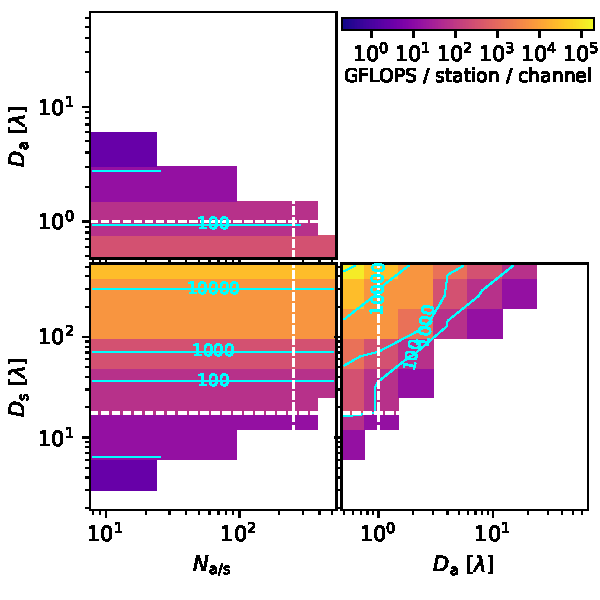
\includegraphics[width=0.48\textwidth]{figures/multidim_epic_cost_analysis_SKA1-low.pdf}}
% \subfloat[][Two-dimensional slices (relative)\label{fig:multidim-incoherent-relative-compcost-EPIC-SKA-low}]{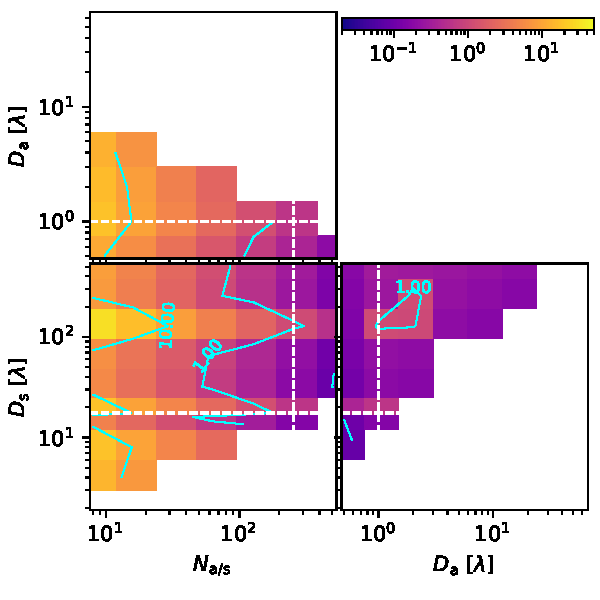
\includegraphics[width=0.48\textwidth]{figures/multidim_epic_relative_cost_analysis_SKA1-low.pdf}}
% \caption{(Left): Two-dimensional slices of the computational cost for coherent-incoherent imaging using station-level EPIC for \texttt{SKA-low}. Cyan contours  \label{fig:incoherent-compcost-EPIC-SKA-low}}
% \end{figure*}

% \begin{figure}
% 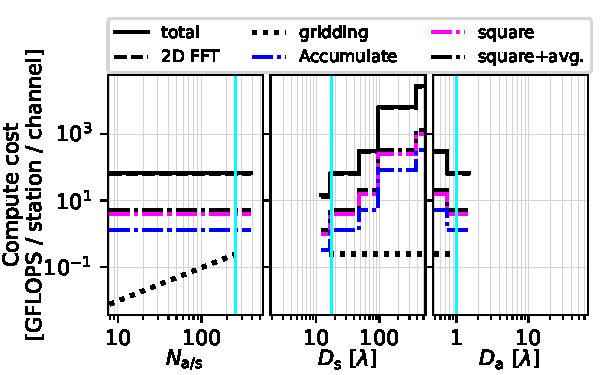
\includegraphics[width=\linewidth]{figures/1D_epic_cost_analysis_SKA1-low.pdf}
% % 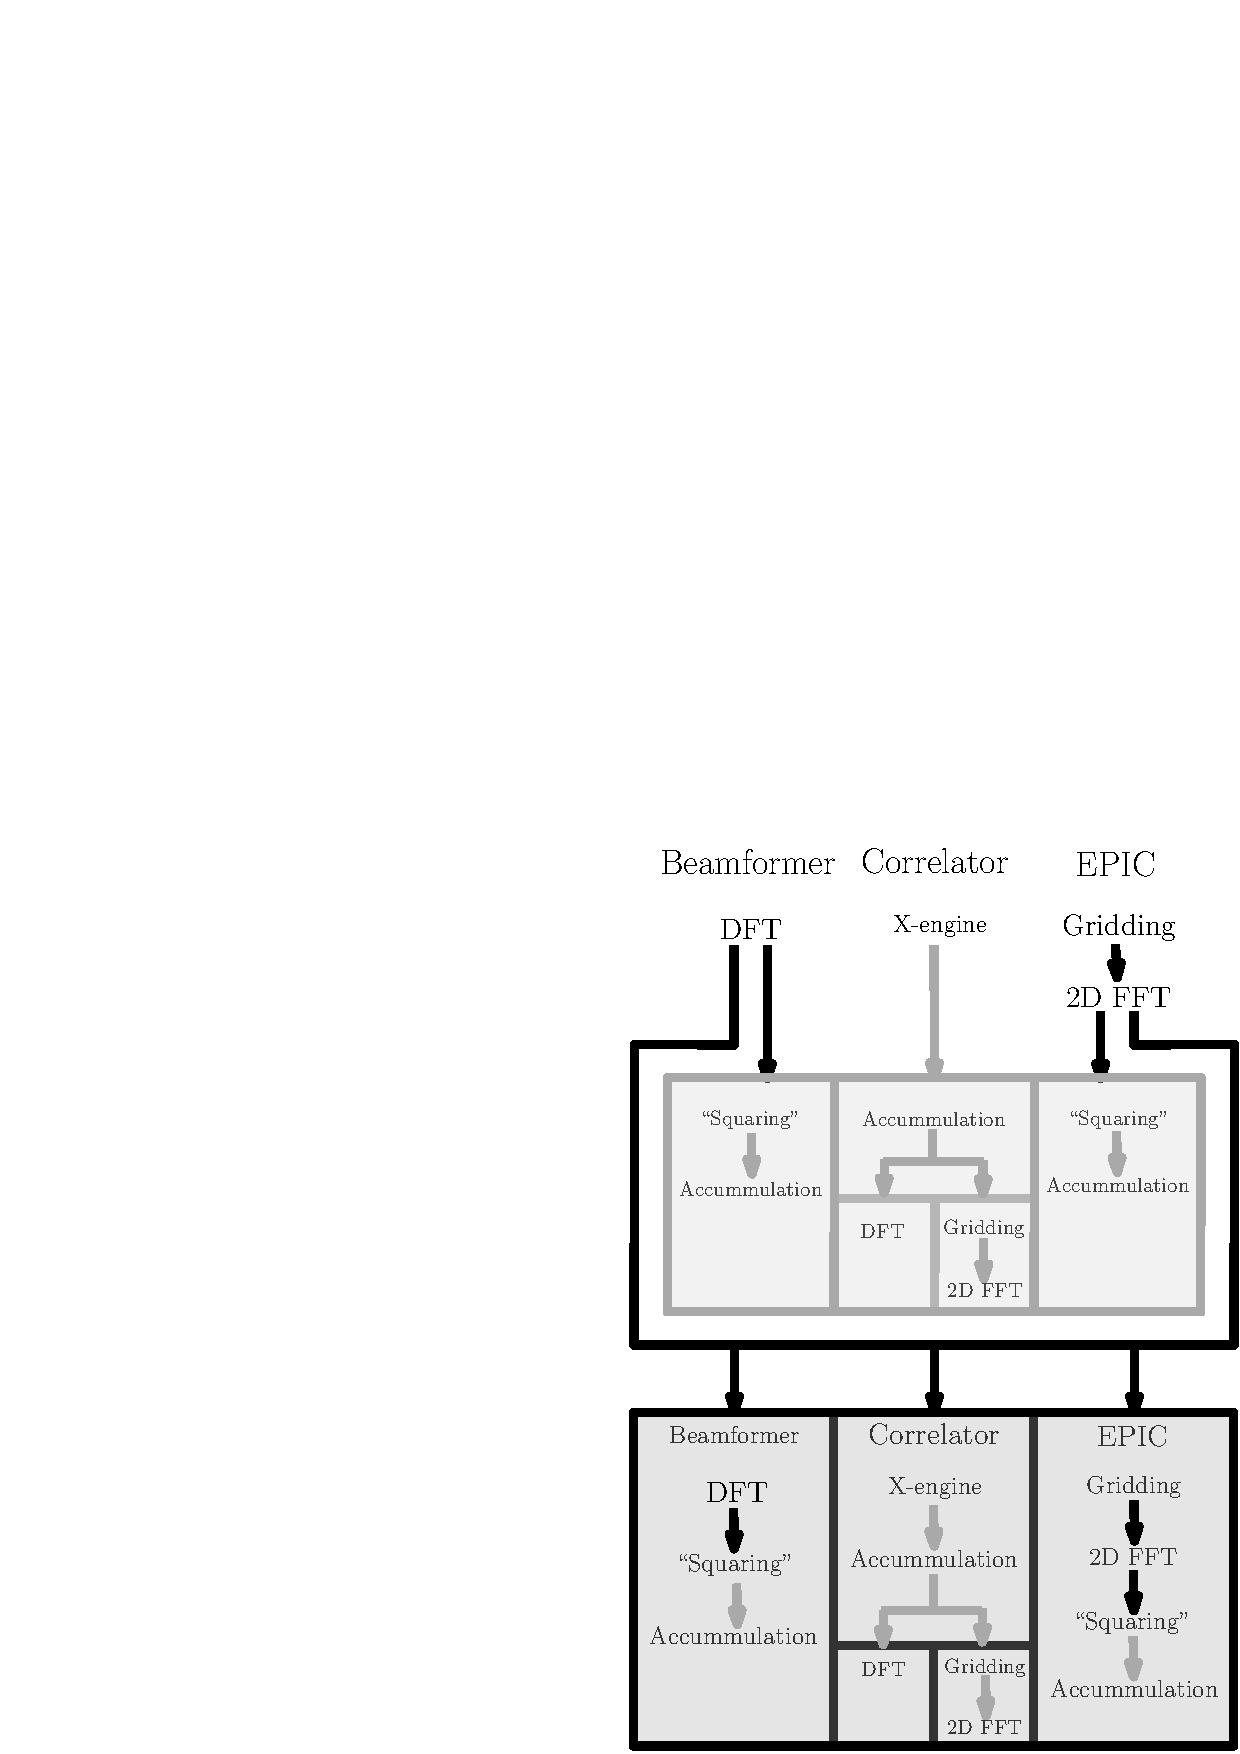
\includegraphics[width=\linewidth]{fig_01.pdf}
% \caption{
% \label{fig:1D-incoherent-compcost-EPIC-SKA-low}}
% \end{figure}

% \subsubsection{Correlator Beamforming (XBF)}

% Calibrated visibilities, $\widetilde{V}_{a_m b_m}^{pq}$, in a station, $m$, can be beamformed through a discrete Fourier transform (DFT) to obtain intensities in any desired direction, $\boldsymbol{s}_k$, as
% \begin{align}
%     \widetilde{\mathcal{I}}_m^{\alpha\beta}(\hat{\boldsymbol{s}}_k) 
%     &= \sum_{a_m,b_m} \sum_{p,q} \widetilde{\mathcal{B}}_{a_m b_m}^{*pq;\alpha\beta}(\hat{\boldsymbol{s}}_k) \, \widetilde{V}_{a_m b_m}^{pq} \,  e^{i\frac{2\pi}{\lambda} \hat{\boldsymbol{s}}_k\cdot\Delta\boldsymbol{r}_{a_m b_m}} \, , \label{eqn:pol-xbf-img-expl} 
% \end{align}
% where, $a_m$ and $b_m$ are elements $a$ and $b$ in station $m$. $\widetilde{\mathcal{B}}_{a_m b_m}^{*pq;\alpha\beta}(\hat{\boldsymbol{s}}_k)$ denotes a complex-valued directional weighting applied to the calibrated visibility and can be chosen to produce images with desired characteristics \citep{Masui+2019}. 
% % This correlation beamforming step can be executed at a cadence of $\Delta t$. However, the correlations that produce visibilities must still be executed on timescales of $\delta t$. Like voltage beamforming, the number of independent beams filling the field of view is $n_\textrm{bs} \simeq (D_\textrm{s}/D_\textrm{a})^2$. 

% The computational cost budget consists of the following components. The formation of polarimetric visibilities and their accumulations requires $n_\textrm{p}^2 N_\textrm{a/s} (N_\textrm{a/s}-1)/2$ complex multiplications and complex additions, respectively, per station per channel at a cadence of $\delta t$. These accumulated visibilities will be further averaged across stations but on a slower cadence of $\Delta t$. However, in order to obtain stationwise image intensities, we will not consider averaging across stations. Thus, the computational cost of forming polarimetric visibilities and their accumulations per station per channel is $4 n_\textrm{p}^2 N_\textrm{a/s} (N_\textrm{a/s}-1)/(\delta t)$ FLOPS. The accumulated visibilities from a station can be beamformed towards $n_\textrm{bs}\simeq (D_\textrm{s}/D_\textrm{a})^2$ sky locations using a DFT to obtain Stokes intensities. This DFT beamforming performs $n_\textrm{p}^2 N_\textrm{a/s} (N_\textrm{a/s}-1) (D_\textrm{s}/D_\textrm{a})^2 /2$ CMACs at a slower cadence of $\Delta t$. Hence, the net computational cost for DFT beamforming of visibilities across the field of view per station per channel is 
% \begin{align}
%     C_\textrm{XBF} &= 4 n_\textrm{p}^2 \, N_\textrm{a/s} (N_\textrm{a/s}-1) \left[\frac{1}{\delta t} + \frac{\left(D_\textrm{s}/D_\textrm{a}\right)^2}{\Delta t} \right] \, . \label{eqn:cost-XBF}
% \end{align}


% \begin{figure*}
% \centering
% \subfloat[][Two-dimensional slices \label{fig:multidim-incoherent-compcost-XBF-SKA-low}]{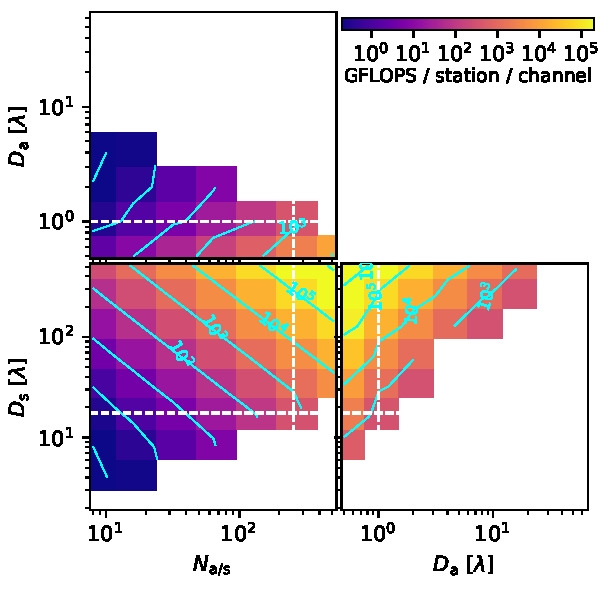
\includegraphics[width=0.48\textwidth]{figures/multidim_xcor_dft_cost_analysis_SKA1-low.pdf}}
% \subfloat[][Two-dimensional slices (relative)\label{fig:multidim-incoherent-relative-compcost-XBF-SKA-low}]{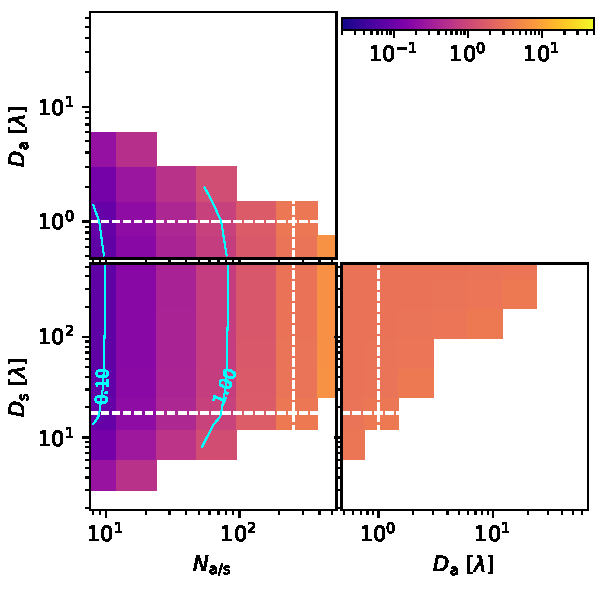
\includegraphics[width=0.48\textwidth]{figures/multidim_xcor_dft_relative_cost_analysis_SKA1-low.pdf}}
% \caption{(Left): Two-dimensional slices of the computational cost for coherent-incoherent imaging using a DFT of station-level cross-correlations for \texttt{SKA-low-core}, \texttt{SKA-low}, \texttt{Aus-VLBA-low}, and \texttt{IC-VLBA-low}. Cyan contours  \label{fig:incoherent-compcost-XBF-SKA-low}}
% \end{figure*}

% \begin{figure}
% 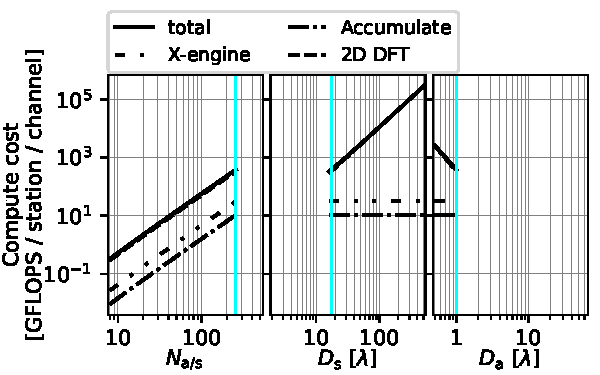
\includegraphics[width=\linewidth]{figures/1D_xcor_dft_cost_analysis_SKA1-low.pdf}
% % 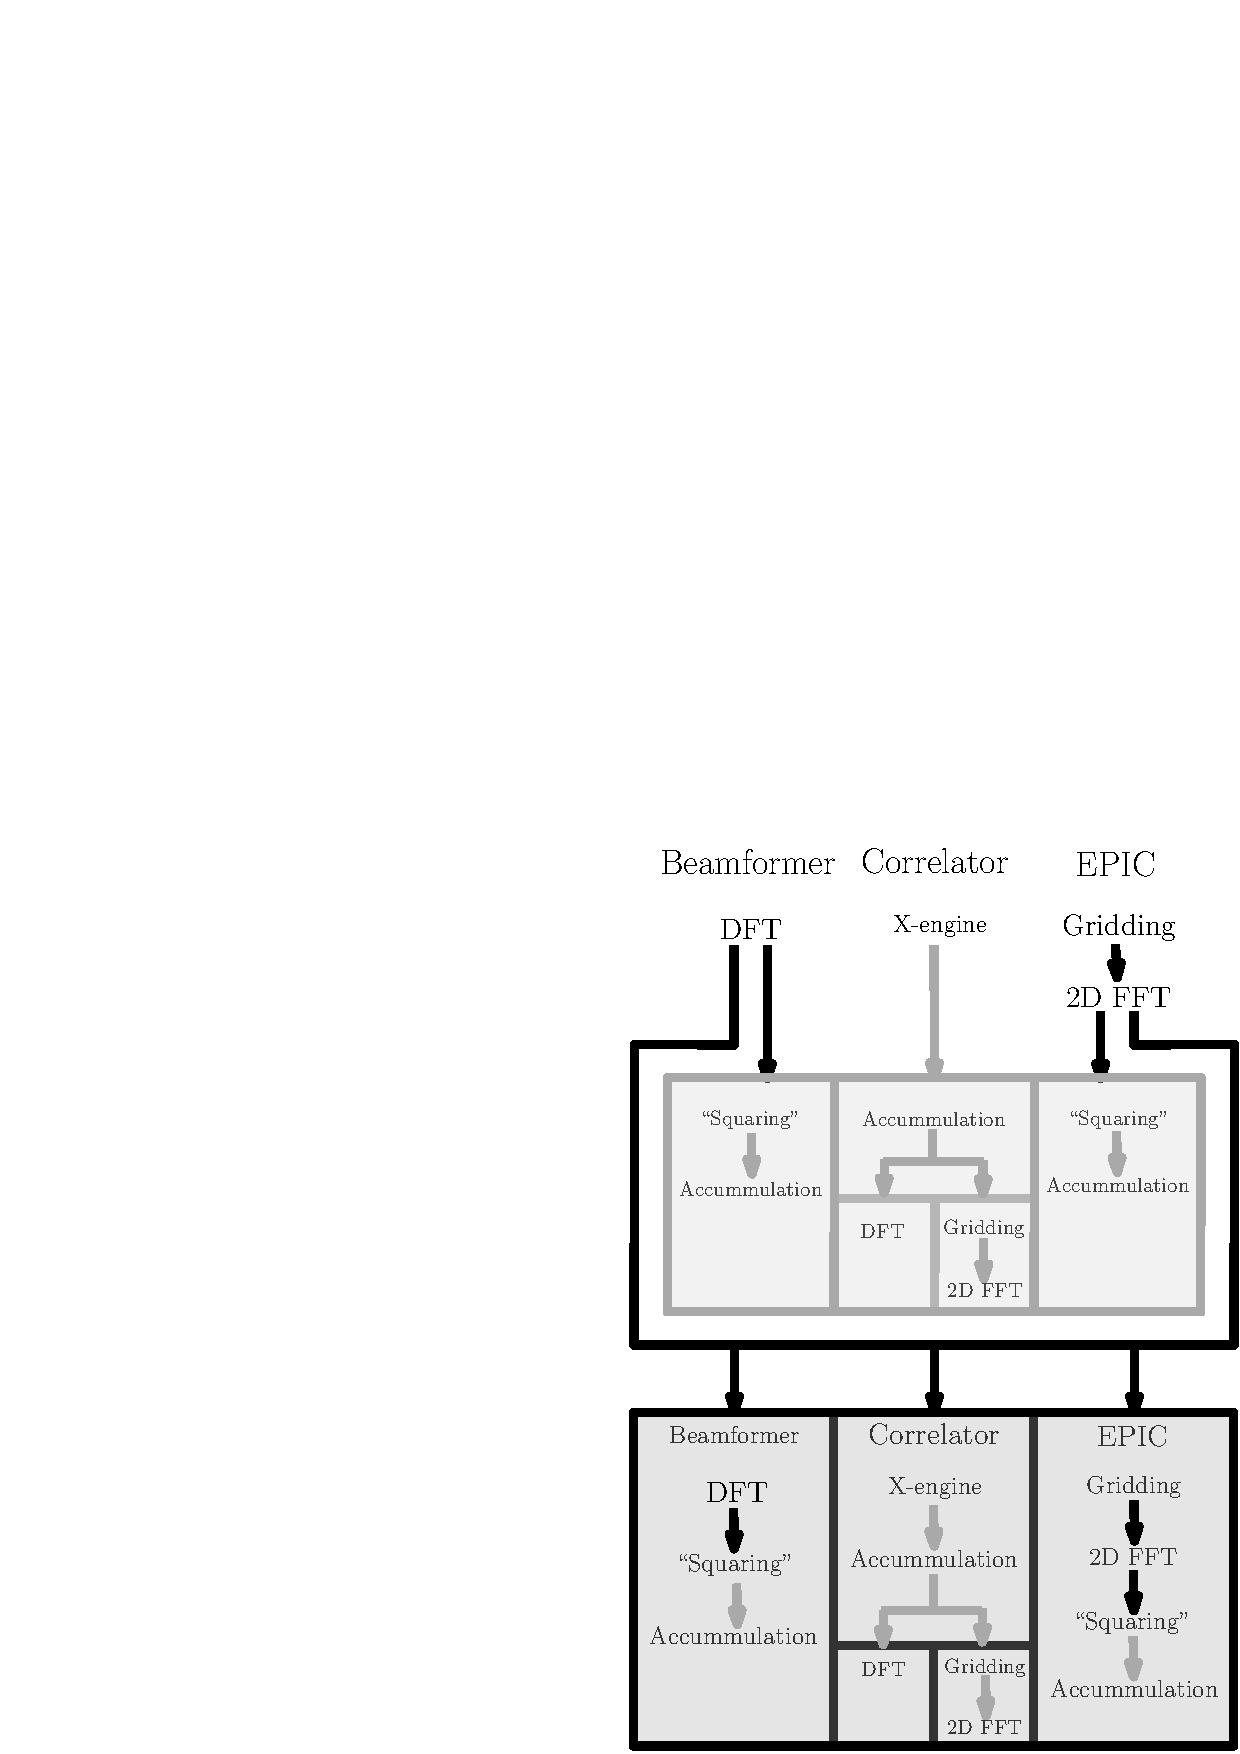
\includegraphics[width=\linewidth]{fig_01.pdf}
% \caption{
% \label{fig:1D-incoherent-compcost-XBF-SKA-low}}
% \end{figure}

% \subsubsection{Correlation and FFT (XFFT)}

% Here, the calibrated visibilities, $\widetilde{V}_{a_m b_m}^{pq}$, in a station, $m$, are gridded and Fourier transformed rather Discrete Fourier transform of correlator beamforming. Mathematically, it is similar to the operations performed on calibrated electric fields from the elements in EPIC, with two key differences -- (1) the calibrated visibilities can be accumulated and allowed for Earth rotation and bandwidth synthesis, (2) the gridding and spatial Fourier transform operates on visibilities rather than electric fields, and (2) the spatial Fourier transform can occur on a slower cadence of $\Delta t$ or the calibration timescale, whichever is shorter. 

% The optimal map-making (OMM) formalism \citep{Tegmark1997a} provides a lossless and optimal (least-squares) solution, which in the radio interferometric context is often referred to as the ``dirty image'' \citep{TMS2017,SIRA-II}, and can be expressed linear algebraically as \citep{Bhatnagar+2008,Morales+2009}:
% \begin{align}
%     \widetilde{\mathbf{I}}_{[m,\hat{\boldsymbol{s}}]} &=  \mathbf{F}^\textrm{H}_{[\hat{\boldsymbol{s}}\leftarrow\Delta\boldsymbol{r}]}\,\widetilde{\mathbf{B}}^\textrm{H}_{[\Delta\boldsymbol{r}\leftarrow\Delta\boldsymbol{r}_{a_m b_m}]} \nonumber\\ 
%     &\qquad \mathbf{N}^{-1}_{[\Delta\boldsymbol{r}_{a_m b_m}\leftarrow\Delta\boldsymbol{r}_{a_m b_m}]}\,\widehat{\mathbf{V}}_{[\Delta\boldsymbol{r}_{a_m b_m}]} \label{eqn:opt-copolar-corr-image}
%     % &= \mathbf{F}^\textrm{H}_{[\hat{\boldsymbol{s}}\leftarrow\Delta\boldsymbol{r}]}\,\mathbf{B}^\textrm{H}_{[\Delta\boldsymbol{r}\leftarrow\Delta\boldsymbol{r}_{a_m b_m}]}\,\mathbf{N}^{-1}_{[\Delta\boldsymbol{r}_{a_m b_m}\leftarrow\Delta\boldsymbol{r}_{a_m b_m}]} \nonumber\\ 
%     % &\qquad\qquad\qquad \vect\left(\Bigl\langle\widehat{\mathbf{E}}_{[\boldsymbol{r}_{a_m}]}\widehat{\mathbf{E}}^\textrm{H}_{[\boldsymbol{r}_{b_m}]}\Bigl\rangle\right)_{[\Delta\boldsymbol{r}_{a_m b_m}]} \, . \label{eqn:opt-copolar-corr-image}
% \end{align}
% The subscript, $m$, on the left hand side denotes that the image was made using measurements within the station, $m$. The inversion operation above takes a column vector of calibrated visibilities, $\widehat{\mathbf{V}}_{[\Delta\boldsymbol{r}_{a_m b_m}]}\coloneqq \vect\left(\Bigl\langle\widehat{\mathbf{E}}_{[\boldsymbol{r}_{a_m}]}\widehat{\mathbf{E}}^\textrm{H}_{[\boldsymbol{r}_{b_m}]}\Bigl\rangle\right)$ at element spacings, $\Delta\boldsymbol{r}_{a_m b_m}$, in station $m$, weights them by the inverse noise covariance, $\mathbf{N}_{[\Delta\boldsymbol{r}_{a_m b_m}\leftarrow\Delta\boldsymbol{r}_{a_m b_m}]}\coloneqq \langle \boldsymbol{n}_{[\Delta\boldsymbol{r}_{a_m b_m}]}\boldsymbol{n}^\textrm{H}_{[\Delta\boldsymbol{r}_{a_m b_m}]}\rangle$, then weights and projects this inverse noise-covariance weighted vector of visibilities onto a finely sampled grid denoted by $\Delta\boldsymbol{r}$ using the operator $\widetilde{\mathbf{B}}^\textrm{H}_{[\Delta\boldsymbol{r}\leftarrow\Delta\boldsymbol{r}_{a_m b_m}]}$, and inverse-Fourier transforms using $\mathbf{F}^\textrm{H}_{[\hat{\boldsymbol{s}}\leftarrow\Delta\boldsymbol{r}]}$ to obtain the estimate of the vector of pixelized intensities, $\widetilde{\mathbf{I}}_{[\hat{\boldsymbol{s}}]}$, on $\mathbb{S}$. 

% The use of $\widetilde{\mathbf{B}}^\textrm{H}_{[\Delta\boldsymbol{r}\leftarrow\Delta\boldsymbol{r}_{a_m b_m}]}$ implies the following. First, if $\widetilde{\mathbf{B}}^\textrm{H}=\mathbf{B}^\textrm{H}$ (assumed hereafter, unless specified), then the inversion is lossless and optimal, minimizing noise and the reconstruction error \citep{Tegmark1997a}. This form is very similar to a matched filter. Second, it transforms the inverse noise covariance weighted visibilities at arbitrary locations, $\Delta\boldsymbol{r}_{a_m b_m}$, to finely sampled locations, $\Delta\boldsymbol{r}$, on a grid. If the grid is uniformly sampled, it facilitates efficient inverse Fourier transform using Fast Fourier Transform (FFT) algorithms. Noting that the optimal inversion is weighted by $\widetilde{\mathbf{B}}^\textrm{H}$, which is the conjugate of that in the RIME in Equation~(\ref{eqn:RIME-LA}), the phase introduced by the instrument is cancelled out precisely during the inversion. However, the amplitude is not. Hence, the inverted image, $\widetilde{\mathbf{I}}_{[\hat{\boldsymbol{s}}]}$, is attenuated relative to the true image, $\mathbf{I}_{[\hat{\boldsymbol{s}}]}$, by a factor that is square of the interferometer's angular power pattern \citep{Bhatnagar+2008,Morales+2009}, once due to $\mathbf{B}_{[\Delta\boldsymbol{r}_{a_m b_m}\leftarrow\Delta\boldsymbol{r}]}$ in Equation~(\ref{eqn:RIME-LA}) (inherent in the measurement) and once more due to $\widetilde{\mathbf{B}}^\textrm{H}_{[\Delta\boldsymbol{r}\leftarrow\Delta\boldsymbol{r}_{a_m b_m}]}$ in Equation~(\ref{eqn:opt-copolar-corr-image}). 

% \begin{figure*}
% \centering
% \subfloat[][Two-dimensional slices \label{fig:multidim-incoherent-compcost-XFFT-SKA-low}]{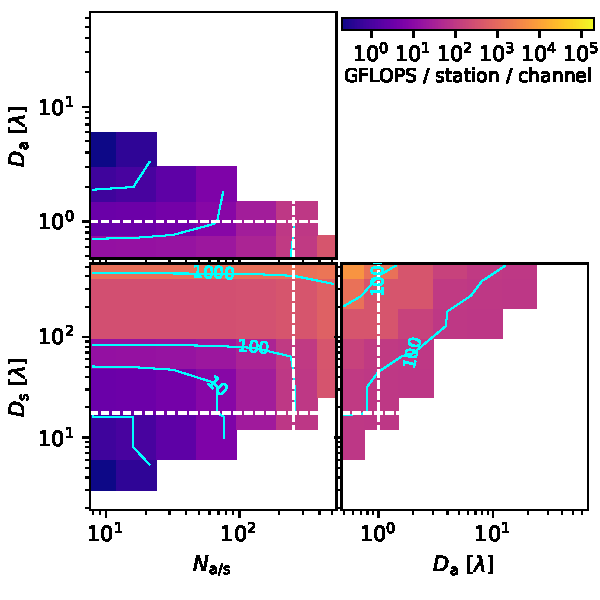
\includegraphics[width=0.48\textwidth]{figures/multidim_xcor_fft_cost_analysis_SKA1-low.pdf}}
% \subfloat[][Two-dimensional slices (relative)\label{fig:multidim-incoherent-relative-compcost-XFFT-SKA-low}]{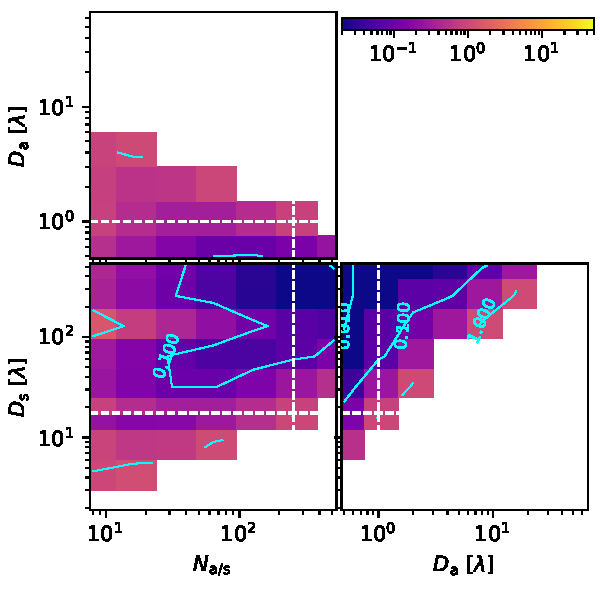
\includegraphics[width=0.48\textwidth]{figures/multidim_xcor_fft_relative_cost_analysis_SKA1-low.pdf}}
% \caption{(Left): Two-dimensional slices of the computational cost for coherent-incoherent imaging using an FFT of station-level cross-correlations for \texttt{SKA-low-core}, \texttt{SKA-low}, \texttt{Aus-VLBA-low}, and \texttt{IC-VLBA-low}. Cyan contours  \label{fig:incoherent-compcost-XFFT-SKA-low}}
% \end{figure*}

% \begin{figure}
% 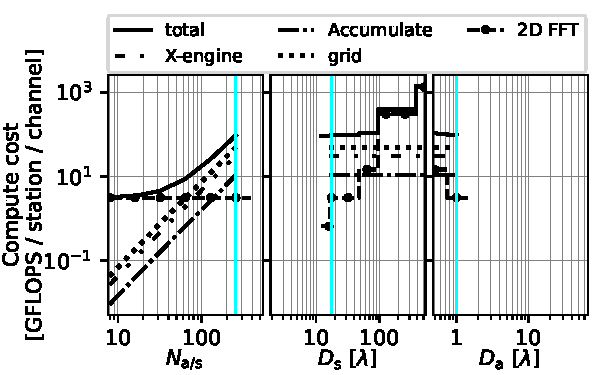
\includegraphics[width=\linewidth]{figures/1D_xcor_fft_cost_analysis_SKA1-low.pdf}
% % 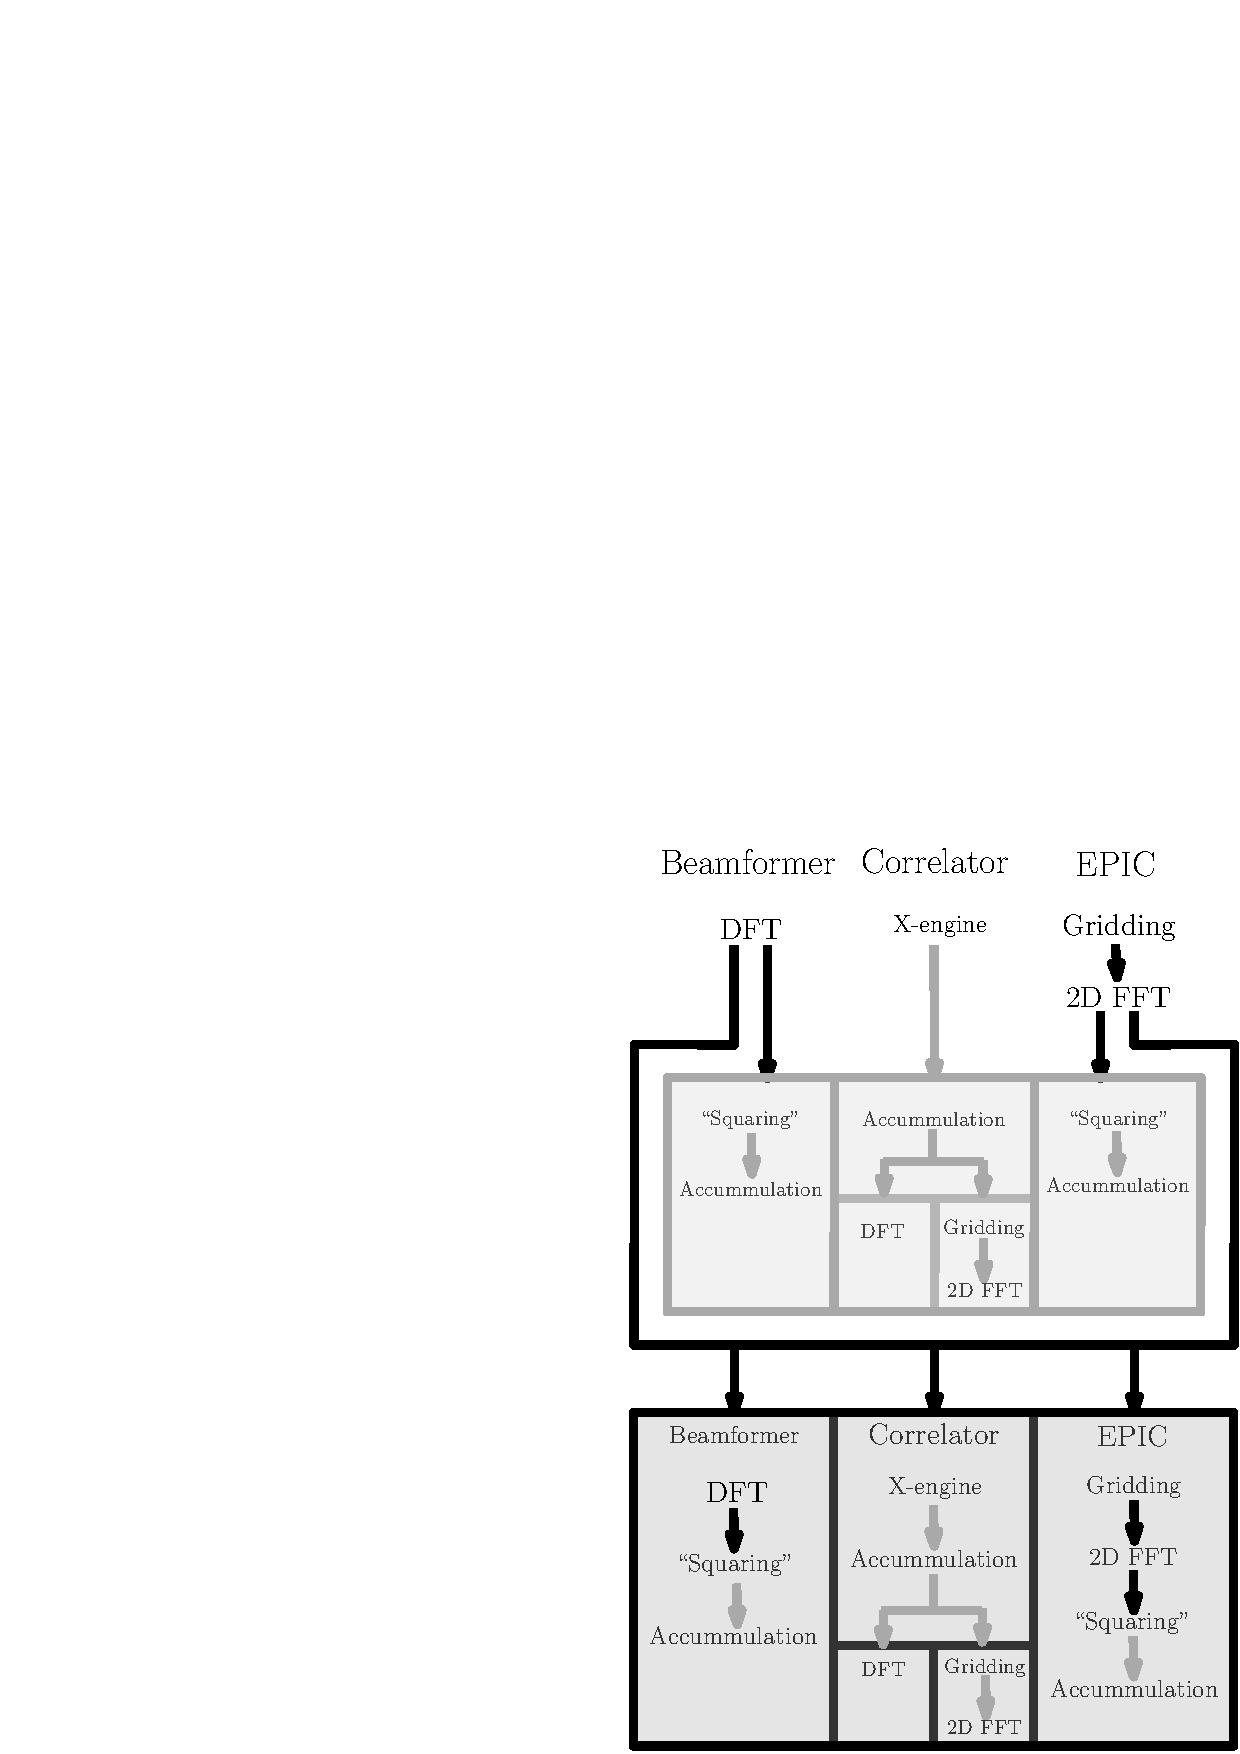
\includegraphics[width=\linewidth]{fig_01.pdf}
% \caption{
% \label{fig:1D-incoherent-compcost-XFFT-SKA-low}}
% \end{figure}

% \begin{figure}
% \centering
% \subfloat[][One-dimensional slices \label{fig:1D-incoherent-compcost-SKA-low}]{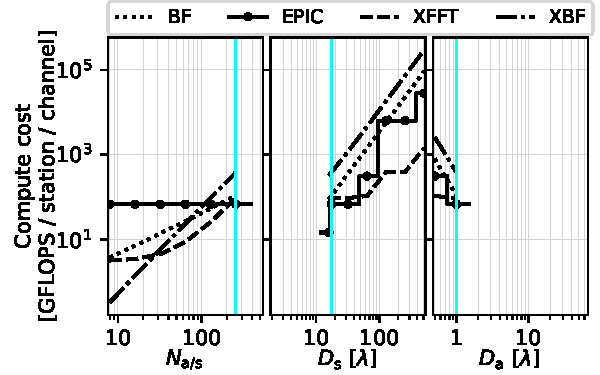
\includegraphics[width=\textwidth]{figures/1D_compcost_analysis_SKA1-low.pdf}} \\
% \subfloat[][One-dimensional slices (relative)\label{fig:1D-incoherent-compcost-XFFT-IC-VLBA-low}]{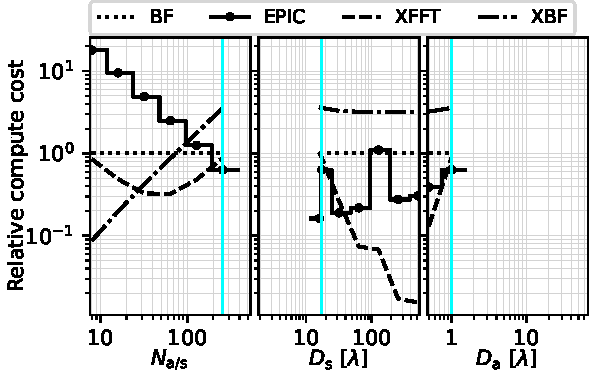
\includegraphics[width=\textwidth]{figures/1D_relative_compcost_analysis_SKA1-low.pdf}}
% \caption{(Left): One-dimensional slices of the computational cost for coherent-incoherent imaging using station-level voltage beamforming for \texttt{SKA-low-core}, \texttt{SKA-low}, \texttt{Aus-VLBA-low}, and \texttt{IC-VLBA-low}. Cyan contours  \label{fig:1D-incoherent-compcost-SKA-low}}
% \end{figure}

% \subsection{Stage II: Inter-station Architectures} \label{sec:inter-station-arch}

% \subsubsection{Incoherent Architectures} \label{sec:incoherent}

% \subsubsection{Coherent Architectures} \label{sec:coherent}

% \subsubsection{Beamforming -- Beamforming (1BF+2BF)}

% \subsubsection{Beamforming -- EPIC (1BF+2EPIC)}

% \subsubsection{Beamforming -- Correlator Beamforming (1BF+2XBF)}

% \subsubsection{Beamforming -- Correlation FFT (1BF+2XFFT)}

% \begin{figure*}
% 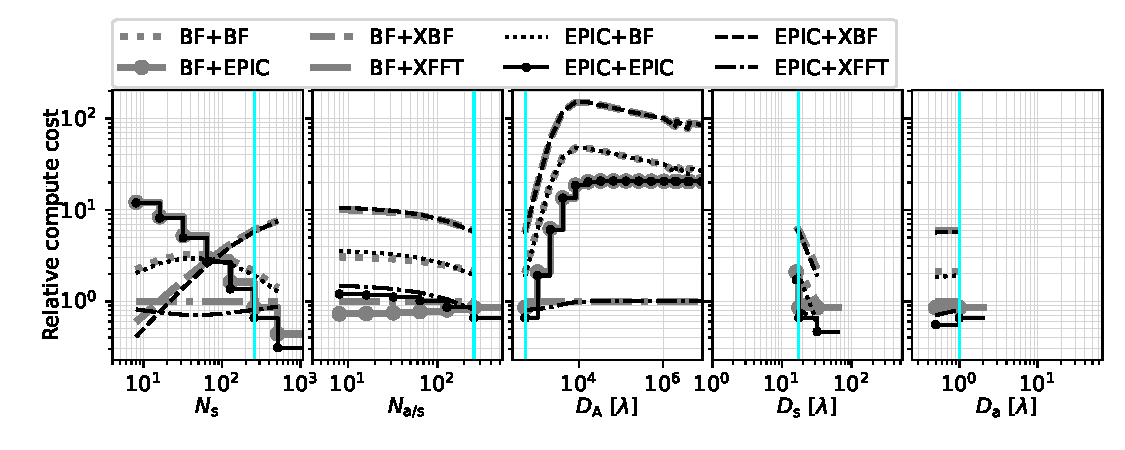
\includegraphics[width=0.95\textwidth]{figures/1D_coherent_relative_compcost_analysis_SKA1-low-core.pdf} 
% \caption{Computational cost of coherent strategy for \texttt{SKA-low-core} relative to BF+XFFT strategy. \label{fig:1D-coherent-relative-compcost-SKA-low-core}}
% \end{figure*}

% \begin{figure*}
% 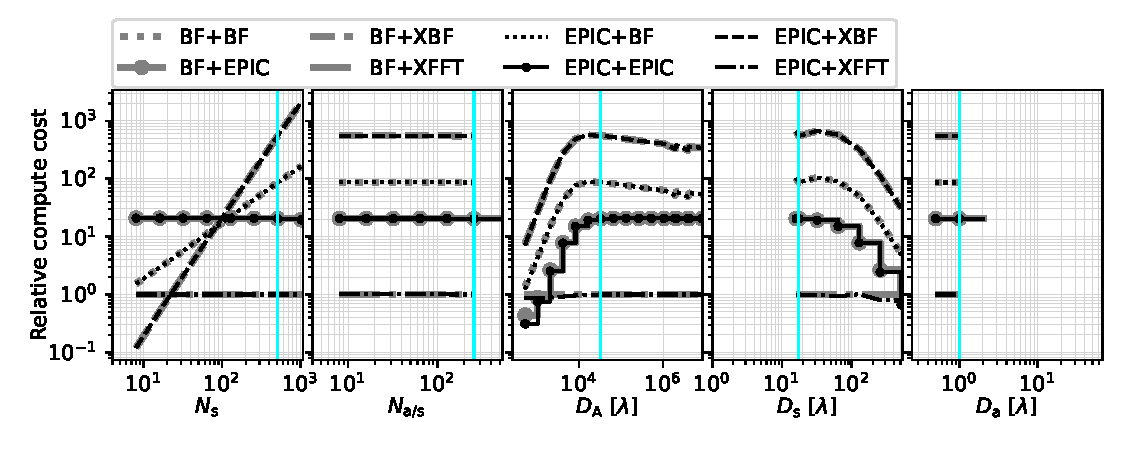
\includegraphics[width=0.95\textwidth]{figures/1D_coherent_relative_compcost_analysis_SKA1-low.pdf}
% \caption{Computational cost of coherent strategy for \texttt{SKA-low} relative to BF+XFFT strategy.  \label{fig:1D-coherent-relative-compcost-SKA-low}}
% \end{figure*}

% \begin{figure*}
% 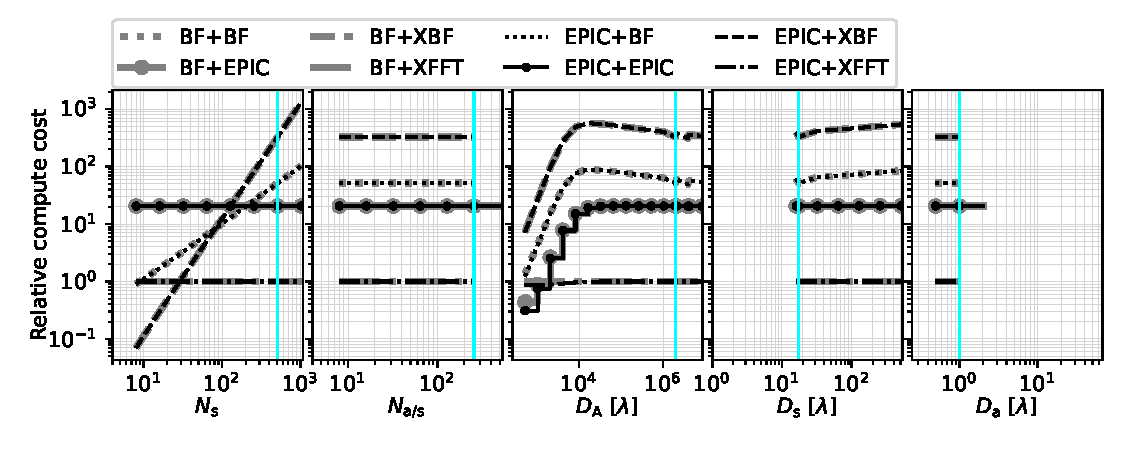
\includegraphics[width=0.95\textwidth]{figures/1D_coherent_relative_compcost_analysis_AU-VLBA-low.pdf}
% \caption{Computational cost of coherent strategy for \texttt{Aus-VLBA-low} relative to BF+XFFT strategy. \label{fig:1D-coherent-relative-compcost-Aus-VLBA-low}}
% \end{figure*}

% \begin{figure*}
% 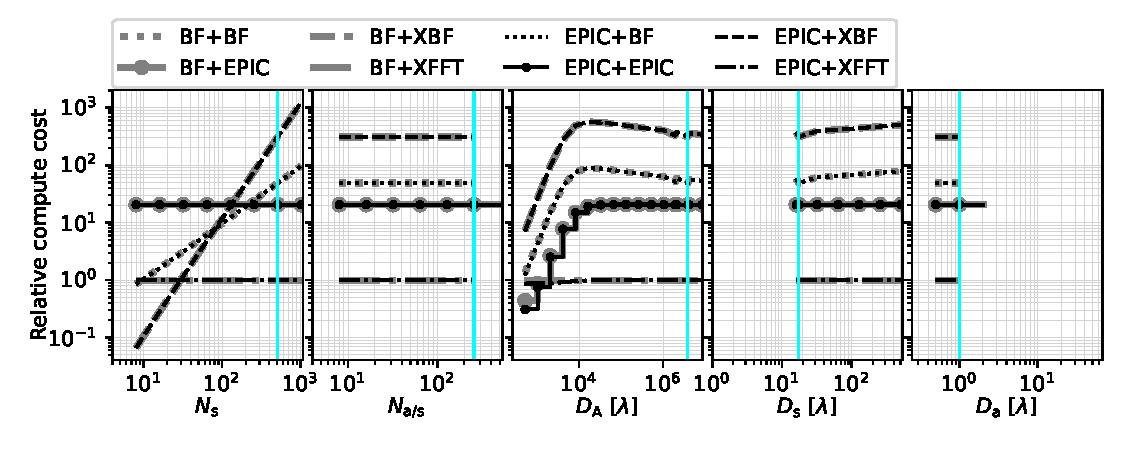
\includegraphics[width=0.95\textwidth]{figures/1D_coherent_relative_compcost_analysis_IC-VLBA-low.pdf}
% \caption{Computational cost of coherent strategy for \texttt{IC-VLBA-low} relative to BF+XFFT strategy. \label{fig:1D-coherent-relative-compcost-IC-VLBA-low}}
% \end{figure*}

\section{Results \& Discussion} \label{sec:results}

\subsection{LAMBDA-I}

\subsection{SKA-low}

\subsection{SKA-low Core}

\subsection{CASPA}

\subsection{FarView}

% \subsection{Australian VLBA-low}

% \subsection{Inter-continental VLBA-low}

\section{Conclusions} \label{sec:conclusion}

% \section{Equations}

% Sample equations. Lorem ipsum dolor sit amet, consectetur adipiscing elit, sed do eiusmod tempor incididunt ut labore et dolore magna aliqua. Lorem ipsum dolor sit amet, consectetur\endnote{Another footnote/endnote} adipiscing elit, sed do eiusmod tempor incididunt ut labore et dolore magna aliqua. Lorem ipsum dolor sit amet, consectetur adipiscing elit, sed do eiusmod tempor incididunt ut labore et dolore magna aliqua. 


% %%% Numbered equation
% \begin{equation}
% \begin{aligned}\label{eq:first}
% \frac{\partial u(t,x)}{\partial t} = Au(t,x) \left(1-\frac{u(t,x)}{K}\right)
%  -B\frac{u(t-\tau,x) w(t,x)}{1+Eu(t-\tau,x)},\\
% \frac{\partial w(t,x)}{\partial t} =\delta \frac{\partial^2w(t,x)}{\partial x^2}-Cw(t,x)
% +D\frac{u(t-\tau,x)w(t,x)}{1+Eu(t-\tau,x)},
% \end{aligned}
% \end{equation}

%  Lorem ipsum dolor sit amet, consectetur adipiscing elit, sed do eiusmod tempor incididunt ut labore et dolore magna aliqua. Lorem ipsum dolor sit amet, consectetur adipiscing elit, sed do eiusmod tempor incididunt ut labore et dolore magna aliqua. Lorem ipsum dolor sit amet, consectetur adipiscing elit, sed do eiusmod tempor incididunt ut labore et dolore magna aliqua. 

% \begin{align}\label{eq:another}
% \begin{split}
% \frac{dU}{dt} &=\alpha U(t)(\gamma -U(t))-\frac{U(t-\tau)W(t)}{1+U(t-\tau)},\\
% \frac{dW}{dt} &=-W(t)+\beta\frac{U(t-\tau)W(t)}{1+U(t-\tau)}.
% \end{split}
% \end{align}


% %%%% Unnumbered equation
% \begin{align*}
% &\frac{\partial(F_1,F_2)}{\partial(c,\omega)}_{(c_0,\omega_0)} = \left|
% \begin{array}{ll}
% \frac{\partial F_1}{\partial c} &\frac{\partial F_1}{\partial \omega} \\\noalign{\vskip3pt}
% \frac{\partial F_2}{\partial c}&\frac{\partial F_2}{\partial \omega}
% \end{array}\right|_{(c_0,\omega_0)}\\
% &\quad=-4c_0q\omega_0 -4c_0\omega_0p^2 =-4c_0\omega_0(q+p^2)>0.
% \end{align*}


% \section{Figures \& Tables}

% The output for a single-column figure is in Figure~\ref{fig_sim}.  Lorem ipsum dolor sit amet, consectetur adipiscing elit, sed do eiusmod tempor incididunt ut labore et dolore magna aliqua. Lorem ipsum dolor sit amet, consectetur adipiscing elit, sed do eiusmod tempor incididunt ut labore et dolore magna aliqua. Lorem ipsum dolor sit amet, consectetur adipiscing elit, sed do eiusmod tempor incididunt ut labore et dolore magna aliqua. 

% Lorem ipsum dolor sit amet, consectetur adipiscing elit, sed do eiusmod tempor incididunt ut labore et dolore magna aliqua. Lorem ipsum dolor sit amet, consectetur adipiscing elit, sed do eiusmod tempor incididunt ut labore et dolore magna aliqua. Lorem ipsum dolor sit amet, consectetur adipiscing elit, sed do eiusmod tempor incididunt ut labore et dolore magna aliqua. 

% %See Figure~\ref{fig_wide} for a double-column figure; this is always at the top of a following page.


% \begin{figure}[hbt!]
% \centering
% 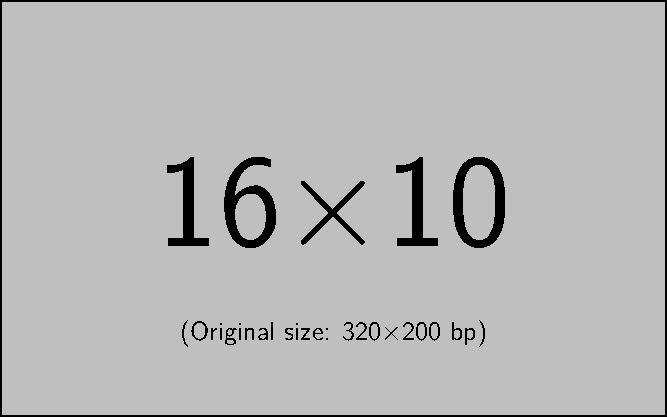
\includegraphics[width=0.75\linewidth]{example-image-16x10.pdf}
% \caption{Insert figure caption here}
% \label{fig_sim}
% \end{figure}


% \begin{figure*}
% \centering
% 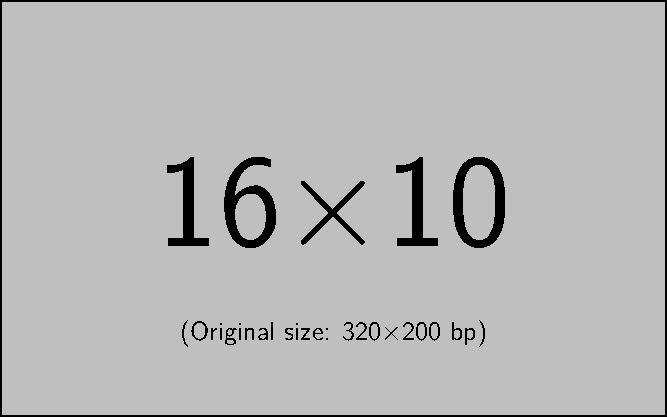
\includegraphics[width=0.8\linewidth]{example-image-16x10.pdf}
% \caption{Insert figure caption here}
% \label{fig_wide}
% \end{figure*}


% See example table in Table~\ref{table_example}.

% \begin{table}[hbt!]
% \begin{threeparttable}
% \caption{An Example of a Table}
% \label{table_example}
% \begin{tabular}{llll}
% \toprule
% \headrow Column head 1 & Column head 2  & Column head 3 & Column head 4\\
% \midrule
% One\tnote{a} & Two&three three &four\\ 
% \midrule
% Three & Four&three three\tnote{b} &four\\
% \bottomrule
% \end{tabular}
% \begin{tablenotes}[hang]
% \item[]Table note
% \item[a]First note
% \item[b]Another table note
% \end{tablenotes}
% \end{threeparttable}
% \end{table}


% \section{Conclusion}
% The conclusion text goes here.


\begin{acknowledgement}
Insert the Acknowledgment text here.
\end{acknowledgement}

% \paragraph{Funding Statement}

% This research was supported by grants from the <funder-name> <doi> (<award ID>); <funder-name> <doi> (<award ID>).

% \paragraph{Competing Interests}

% A statement about any financial, professional, contractual or personal relationships or situations that could be perceived to impact the presentation of the work --- or `None' if none exist.

% \paragraph{Data Availability Statement}

% A statement about how to access data, code and other materials allowing users to understand, verify and replicate findings --- e.g. Replication data and code can be found in Harvard Dataverse: \verb+\url{https://doi.org/link}+.

%\endnote in some journals will behave like \footnote; and \printendnotes will not output anything. 
\printendnotes

% \printbibliography
\bibliography{refs}

\appendix

\section{Mathematical Details of Architectures}

\subsection{Co-polar Interferometry}\label{sec:copolar-interferometry}

If we represent $\mathcal{E}^\alpha(\hat{\boldsymbol{s}},\nu,t)$ as the spectral Fourier components, $\nu$, of the time-domain electric fields, $\mathcal{E}_{t^\prime}(\alpha,\hat{\boldsymbol{s}},t^\prime)$, emanating from astrophysical sources of emission in directions denoted by the unit vector, $\hat{\boldsymbol{s}}$ measured over a finite time interval, $T$, centered around time, $t$, then:
\begin{align}
    \mathcal{E}^\alpha(\hat{\boldsymbol{s}},\nu,t) = \frac{1}{T}\int\limits_{t-T/2}^{t+T/2} \mathcal{E}_{t^\prime}^\alpha(\hat{\boldsymbol{s}},t^\prime) e^{-i 2\pi \nu t^\prime} \mathrm{d}t^\prime,
\end{align}
where, superscript $\alpha\in\{1,2\}$ denotes the polarisation state of the radiation, $\nu$ denotes the spectral component or the frequency of radiation, $\lambda=c/\nu$ is the wavelength, where $c$ is the speed of light. Because all the operations considered in this paper operate independently on each spectral channel, $\nu$, and time, $t$, we will hereafter assume implicit dependence on $\nu$ and $t$ throughout without explicitly specifying it. 

A measuring instrument, like an antenna in an aperture array, in the aperture plane will measure the superposition of these electric fields as they propagate from the sky locations spanning the celestial surface, $\mathbb{S}$, while imprinting its transfer function, $\mathcal{W}_{a_m}^{p\alpha}(\hat{\boldsymbol{s}})$, as
\begin{align}
    \underline{E}_{a_m}^p &= \int_\mathbb{S} \sum_\alpha  \mathcal{W}_{a_m}^{p\alpha}(\hat{\boldsymbol{s}})\, \mathcal{E}^\alpha(\hat{\boldsymbol{s}})\, e^{-i \frac{2\pi}{\lambda} \hat{\boldsymbol{s}}\cdot\boldsymbol{r}_{a_m}} \,\mathrm{d}\Omega \, , \label{eqn:polarimetric-Efield-element-ideal}
\end{align}


Electric fields in the aperture plane, $\underline{E}(\boldsymbol{r})$, can be written as a superposition of those that propagated from the astrophysical sources on the celestial surface $\mathbb{S}$, $\mathcal{E}(\hat{\boldsymbol{s}})$:
\begin{align}
    \underline{E}(\boldsymbol{r}) &= \int_\mathbb{S} \mathcal{E}(\hat{\boldsymbol{s}})\, e^{-i \frac{2\pi}{\lambda}\hat{\boldsymbol{s}}\cdot\boldsymbol{r}} \,\mathrm{d}\Omega,
\end{align}
where, the integral is over the celestial surface, $\mathbb{S}$, covered by the unit vector, $\hat{\boldsymbol{s}}$, $\boldsymbol{r}$ denotes the observer's location, $t$ denotes time, $\mathrm{d}\Omega=\mathrm{d}^2\hat{\boldsymbol{s}}$ is the infinitesimal solid angle element on the tangent plane of the celestial sphere perpendicular to the unit vector $\hat{\boldsymbol{s}}$. 

Thus, the propagated electric field can be construed as a linear superposition of the electric fields emanating from astronomical sources with appropriate complex phases acquired during the propagation. Ignoring wide-field effects, this relation can be simplified as a Fourier transform of the electric fields in the sky coordinates. 

% In the presence of a directional response of an ideal instrument, which includes but is not limited to the directional electric field pattern of the element, the electric field measured by the 

In order to generalize later, we will consider a station indexed by $m$ as being made up of a group of $N_m$ elements, indexed by $a_m$. For now, we will focus on a single station, denoted by $m$. 

The measuring instrument will imprint its transfer function on the measurements. If $\mathcal{W}_{a_m}(\hat{\boldsymbol{s}})$ is the directional electric field response of the element, $a_m$, then the electric field measured by this element will be ideally
\begin{align}
    \underline{E}_{a_m} &= \int_\mathbb{S} \mathcal{W}_{a_m}(\hat{\boldsymbol{s}})\, \mathcal{E}(\hat{\boldsymbol{s}})\, e^{-i \frac{2\pi}{\lambda} \hat{\boldsymbol{s}}\cdot\boldsymbol{r}_{a_m}} \,\mathrm{d}\Omega \, . \label{eqn:copolar-Efield-element-ideal}
\end{align}
In the typical case of non-ideal behavior of an element, the measured electric field will be potentially corrupted both in amplitude and phase relative to the ideal measurement in Equation~(\ref{eqn:copolar-Efield-element-ideal}). Then,
\begin{align}
    E_{a_m} &= g_{a_m}\underline{E}_{a_m} + n_{a_m} \, , \label{eqn:Efield-element}
\end{align}
where, $g_{a_m}$ denotes the multiplicative complex gain encapsulating the corruption of the wavefront due to instrumental and propagation effects, and $n_{a_m}$ denotes element-based additive noise in the measurement chain. A process of calibration is typically performed to remove the effects of this corruption by obtaining the best estimate, $\widehat{g}_{a_m}$, of the corrupting gain term, $g_{a_m}$, and the estimated electric field at the element after calibration will be:
\begin{align}
    \widehat{\underline{E}}_{a_m} &= \widehat{g}_{a_m}^{-1}\,E_{a_m} \, . \label{eqn:calibration}
\end{align}


% then $\mathcal{W}_{a_m}(\hat{\boldsymbol{s}})$ is the corresponding directional electric field response of the element. Thus, by application of Fourier transform properties, 
% \begin{align}
%     E_{a_m}^\textrm{I} &= \int_\mathbb{S} \mathcal{W}_{a_m}(\hat{\boldsymbol{s}})\, \mathcal{E}(\hat{\boldsymbol{s}})\, e^{-2\pi i\frac{\nu}{c} \boldsymbol{r}\cdot \hat{\boldsymbol{s}}} \,\mathrm{d}\Omega
% \end{align}


% \begin{align}
%     &= \int_\mathbb{R} W_{a_m}(\boldsymbol{r} - \boldsymbol{r}_{a_m}) \nonumber\\
%     &\quad \times \left[\int_\textrm{S} \mathcal{E}(\hat{\boldsymbol{s}})\, e^{-2\pi i\nu \boldsymbol{r}\cdot \hat{\boldsymbol{s}}/c} \,\mathrm{d}\Omega\right]\, \mathrm{d}^2 \boldsymbol{r} + n_{a_m} \\
%     &= \int_\textrm{S} \mathcal{W}_{a_m}(\hat{\boldsymbol{s}})\, \mathcal{E}(\hat{\boldsymbol{s}})\, e^{-2\pi i\nu \boldsymbol{r}\cdot \hat{\boldsymbol{s}}/c} \,\mathrm{d}\Omega \nonumber\\ 
%     &\qquad + n_{a_m}  + n_{a_m}
% \end{align}
% The weighting, denoted by $W_{a_m}(\boldsymbol{r})$, encapsulates the aperture field illumination pattern of the element, the complex element gains (including direction-dependence) containing the effects of the propagation medium as well as of the instrumentation. $\mathcal{W}_{a_m}(\hat{\boldsymbol{s}})$ is the spatial Fourier transform of $W_{a_m}(\boldsymbol{r})$. If $W_{a_m}(\boldsymbol{r})$ denotes only the aperture field illumination pattern, then $\mathcal{W}_{a_m}(\hat{\boldsymbol{s}})$ is the corresponding directional element voltage response towards the celestial surface. 

The theory of mutual coherence has established the relation between the intensity distribution of spatially incoherent quasi-monochromatic emission, $I(\hat{\boldsymbol{s}})$ on $\mathbb{S}$ and mutual coherence, or ``true'' visibility, $\underline{V}(\Delta\boldsymbol{r})\coloneqq \bigl\langle \underline{E}(\boldsymbol{r})\underline{E}^*(\boldsymbol{r}+\Delta\boldsymbol{r})\bigr\rangle$, in the aperture plane, and is popularly known as the \textit{Van Cittert-Zernike} theorem \citep{VanCittert1934,Zernike1938,Born-Wolf,Goodman2000,TMS2017}:
\begin{align}
    \underline{V}(\Delta\boldsymbol{r}) &= \int_\mathbb{S} \mathcal{I}(\hat{\boldsymbol{s}})\, e^{-i\frac{2\pi}{\lambda} \hat{\boldsymbol{s}}\cdot\Delta\boldsymbol{r}} \,\mathrm{d}\Omega, \label{eqn:VCZ-theorem}
\end{align}
where, $\Delta\boldsymbol{r}$, denotes the displacement vector between any two locations\footnote{The dependence of spatial coherence on $\Delta\mathbb{R}$ (displacement vectors between the element pairs), rather than $\mathbb{R}$ (absolute positions), in Equation~(\ref{eqn:VCZ-theorem}) implies an assumption of wide-sense spatial stationarity for the electric fields measured on the aperture, which will hold true only when the spatial intensity distribution, $\mathcal{I}(\hat{\boldsymbol{s}})$, on $\mathbb{S}$ is incoherent.} in the aperture domain $\mathbb{R}$, $\langle\cdot\rangle$ denotes an estimator of the ensemble average\footnote{This is typically obtained by assuming ergodicity and averaging over a coherence scale usually along temporal or spectral axes, and sometimes over redundant element spacings.}, and $*$ denotes complex conjugation. When the ideal instrument's transfer function is included in the measurement process, the visibility measured by the interferometer elements $a$ and $b$ (with separation $\Delta\boldsymbol{r}_{a_m b_m}\coloneqq \boldsymbol{r}_{a_m}-\boldsymbol{r}_{b_m}$) will be:
\begin{align}
    \underline{V}_{a_m b_m} &= \int_\mathbb{S} \mathcal{B}_{a_m b_m}(\hat{\boldsymbol{s}})\,\mathcal{I}(\hat{\boldsymbol{s}})\, e^{-i\frac{2\pi}{\lambda} \hat{\boldsymbol{s}}\cdot\Delta\boldsymbol{r}_{a_m b_m}} \,\mathrm{d}\Omega, \label{eqn:ideal-copolar-visibilities}
\end{align}
where, 
\begin{align}
    \mathcal{B}_{a_m b_m}(\hat{\boldsymbol{s}}) &=  \mathcal{W}_{a_m}(\hat{\boldsymbol{s}})\,\mathcal{W}_{b_m}^*(\hat{\boldsymbol{s}}) \, ,
\end{align}
is called the directional cross-power pattern of an ideal two-element interferometer (made of elements $a$ and $b$). Equation~(\ref{eqn:ideal-copolar-visibilities}) is referred to as the radio interferometric measurement equation (RIME). 
% In the absence of other non-ideal effects, $\mathcal{B}_{a_m b_m}(\hat{\boldsymbol{s}})$ corresponds to the directional cross-power pattern of the interferometer comprising of elements $a$ and $b$.

Correlators in interferometer arrays produce complex correlations products of the measured (corrupted) electric fields between pairs of elements (denoted by $a$ and $b$) to produce corrupted visibilities,
\begin{align}
    V_{a_m b_m} &= \bigl\langle E_{a_m} \, E_{b_m}^*\bigr\rangle \\
    &= g_{a_m}\, \underline{V}_{a_m b_m}\, g_{b_m}^* + n_{a_m b_m} \, . \label{eqn:corrupted-noise-visibility}
\end{align}
% where, $\underline{V}_{a_m b_m}$ denotes ideal visibilities measured at element spacing $\boldsymbol{r}_{a_m b_m}\coloneqq \boldsymbol{r}_{a_m}-\boldsymbol{r}_{b_m}$, $\langle\cdot\rangle$ denotes an estimator of the ensemble average\footnote{This is typically obtained by assuming ergodicity and averaging over a coherence scale usually along temporal or spectral axes, and sometimes over redundant element spacings.}, and $*$ denotes complex conjugation. 
The corresponding estimate of ideal visibilities, after calibration, will be
\begin{align}
    \widehat{\underline{V}}_{a_m b_m} &= \bigl\langle \widehat{\underline{E}}_{a_m}\widehat{\underline{E}}_{b_m}^*\bigr\rangle \nonumber\\
    &= \widehat{g}_{a_m}^{-1}\, V_{a_m b_m}\, \widehat{g}_{b_m}^{*^{-1}} \, .
\end{align}
Because this paper does not concern primarily with calibration, we will assume that the measured element electric fields are perfectly calibrated hereafter, and hence, $\widehat{\underline{E}}_{a_m}=\underline{E}_{a_m}$ and $E_{a_m}=\underline{E}_{a_m}+n_{a_m}$. Correspondingly, we will assume $\widehat{\underline{V}}_{a_m b_m}=\underline{V}_{a_m b_m}$ and $V_{a_m b_m}=\underline{V}_{a_m b_m}+n_{a_m b_m}$. 

% Equation~(\ref{eqn:ideal-copolar-visibilities}) can be alternatively expressed in the aperture domain, using Fourier transform properties, as:
% \begin{align}
%     V_{a_m b_m}^\textrm{I} &= \int_{\Delta\mathbb{R}} B_{a_m b_m}(\Delta\boldsymbol{r}-\Delta\boldsymbol{r}_{a_m b_m})\,V^\textrm{T}(\Delta\boldsymbol{r})\,\mathrm{d}^2\Delta\boldsymbol{r}, \label{eqn:vis-degridding}
% \end{align}
% where, $B_{a_m b_m}(\Delta\boldsymbol{r})$ denotes the cross-power illumination of the interferometer's aperture. Equation~(\ref{eqn:vis-degridding}) represents a weighting of the true spatial coherence of the incident radiation by the interferometer's cross-power illumination pattern and integration over the region the interferometer has a response to. $\Delta\mathbb{R}$ denotes the space of all possible displacement vectors between elements. $B_{a_m b_m}(\Delta\boldsymbol{r})$ is the Fourier transform of $\mathcal{B}_{a_m b_m}(\hat{\boldsymbol{s}})$. Thus,
% \begin{align}
%     B_{a_m b_m}(\Delta\boldsymbol{r}) &= \frac{\nu^2}{c^2}\int_\mathbb{S} \mathcal{W}_{a_m}(\hat{\boldsymbol{s}})\mathcal{W}_{b_m}^{*}(\hat{\boldsymbol{s}})\nonumber\\
%     &\qquad\qquad \times e^{-2\pi i\frac{\nu}{c} \Delta\boldsymbol{r}\cdot\hat{\boldsymbol{s}}} \,\mathrm{d}\Omega \\
%     &= \int_\mathbb{R} W_{a_m}(\boldsymbol{r}) W_{b_m}^{*}(\boldsymbol{r}+\Delta\boldsymbol{r})\,\mathrm{d}^2\boldsymbol{r}. \label{eqn:holographic-power-illumination}
% \end{align}
 
% Interferometric image synthesis involves inverting Equation~(\ref{eqn:VCZ-theorem}) to obtain $\mathcal{I}(\hat{\boldsymbol{s}})$, the spatial intensity distribution on $\mathbb{S}$, using a number of calibrated visibility measurements, $\widehat{V}_{a_m b_m}$, from different element pairs. The optimal map-making (OMM) formalism \citep{Tegmark1997a} provides an optimal solution, which in the radio interferometric context is often referred to as the ``dirty image'' \citep{TMS2017,SIRA-II}. In linear algebraic notation, the measurement and the optimal inversion operations can be written as \citep{Bhatnagar+2008,Morales+2009}:
% \begin{align}
%     \mathbf{V}_{[\Delta\boldsymbol{r}_{a_m b_m}]} &= \mathbf{B}_{[\Delta\boldsymbol{r}_{a_m b_m}|\Delta\boldsymbol{r}]}\,\mathbf{F}_{[\Delta\boldsymbol{r}|\hat{\boldsymbol{s}}]}\,\mathbf{I}_{[\hat{\boldsymbol{s}}]} + \mathbf{n}_{[\Delta\boldsymbol{r}_{a_m b_m}]}, \label{eqn:RIME-LA}
% \end{align}
% and
% \begin{align}
%     \widehat{\mathbf{I}}_{[\hat{\boldsymbol{s}}]} &=  \mathbf{F}^\textrm{H}_{[\hat{\boldsymbol{s}}\leftarrow\Delta\boldsymbol{r}]}\,\mathbf{B}^\textrm{H}_{[\Delta\boldsymbol{r}\leftarrow\Delta\boldsymbol{r}_{a_m b_m}]}\,\mathbf{N}^{-1}_{[\Delta\boldsymbol{r}_{a_m b_m}\leftarrow\Delta\boldsymbol{r}_{a_m b_m}]}\,\widehat{\mathbf{V}}_{[\Delta\boldsymbol{r}_{a_m b_m}]} \label{eqn:OptEst-LA} \\
%     &= \mathbf{F}^\textrm{H}_{[\hat{\boldsymbol{s}}\leftarrow\Delta\boldsymbol{r}]}\,\mathbf{B}^\textrm{H}_{[\Delta\boldsymbol{r}\leftarrow\Delta\boldsymbol{r}_{a_m b_m}]}\,\mathbf{N}^{-1}_{[\Delta\boldsymbol{r}_{a_m b_m}\leftarrow\Delta\boldsymbol{r}_{a_m b_m}]} \nonumber\\ 
%     &\qquad\qquad\qquad \vect\left(\Bigl\langle\widehat{\mathbf{E}}_{[\boldsymbol{r}_{a_m}]}\widehat{\mathbf{E}}^\textrm{H}_{[\boldsymbol{r}_{b_m}]}\Bigl\rangle\right)_{[\Delta\boldsymbol{r}_{a_m b_m}]}, \label{eqn:opt-copolar-corr-image}
% \end{align}
% respectively. Here, the dependence on $\nu$ and $t$ have been omitted for convenience as they carry through the equation without transformations. $\vect(\mathbf{M})$ denotes the vectorization of a matrix $\mathbf{M}$ into a column vector. Quantities with a single bracketed variable, such as $\mathbf{V}_{[\Delta\boldsymbol{r}_{a_m b_m}]}$, $\mathbf{I}_{[\hat{\boldsymbol{s}}]}$, $\mathbf{n}_{[\Delta\boldsymbol{r}_{a_m b_m}]}$, and $\widehat{\mathbf{I}}_{[\hat{\boldsymbol{s}}]}$, denote vectors that are a function of that variable, and those with two bracketed variables denote matrix operators that transform the vector between the variable on the right of the delimiter $\leftarrow$ to that on its left. For example, Equation~(\ref{eqn:RIME-LA}) Fourier transforms a vector of true pixelized intensities, $\mathbf{I}_{[\hat{\boldsymbol{s}}]}$, to a spatial coherence function, $\mathbf{F}_{[\Delta\boldsymbol{r}|\hat{\boldsymbol{s}}]}\mathbf{I}_{[\hat{\boldsymbol{s}}]}$, defined on a continuous variable (or finely sampled in case of a discretized implementation), $\boldsymbol{r}_{a_m b_m}$, which through the operator represented by $\mathbf{B}_{[\Delta\boldsymbol{r}_{a_m b_m}|\Delta\boldsymbol{r}]}$ is then further transformed into a discrete vector of measured visibilities between specific element pairs, $\mathbf{V}_{[\Delta\boldsymbol{r}_{a_m b_m}]}$, which includes an additive measurement noise vector, $\mathbf{n}_{[\Delta\boldsymbol{r}_{a_m b_m}]}$. 
% % weighted by $B_{a_m b_m}(\Delta\boldsymbol{r})$ and integrated the propagated spatial coherence over the aperture defined on a continuous (or finely sampled in case of a discretized implementation) variable $\Delta\boldsymbol{r}$ and obtaining the visibility measured at the specific element spacing, $\Delta\boldsymbol{r}_{a_m b_m}$. 
% Equation~(\ref{eqn:OptEst-LA}) represents the optimal inversion operation that takes the vector of measured visibilities that have been calibrated, $\widehat{\mathbf{V}}_{[\Delta\boldsymbol{r}_{a_m b_m}]}$, weights them by the inverse of the noise covariance, $\mathbf{N}_{[\Delta\boldsymbol{r}_{a_m b_m}|\Delta\boldsymbol{r}_{a_m b_m}]}\coloneqq \langle \boldsymbol{n}_{[\Delta\boldsymbol{r}_{a_m b_m}]}\boldsymbol{n}^\textrm{H}_{[\Delta\boldsymbol{r}_{a_m b_m}]}\rangle$, then weights and projects this inverse noise-covariance weighted vector of visibilities onto a finely sampled grid denoted by $\Delta\boldsymbol{r}_{a_m b_m}$ using the operator $\mathbf{B}^\textrm{H}_{[\Delta\boldsymbol{r}|\Delta\boldsymbol{r}_{a_m b_m}]}$, and Fourier transforms to obtain the optimal estimate of the vector of pixelized intensities, $\widehat{\mathbf{I}}_{[\hat{\boldsymbol{s}}]}$, on $\mathbb{S}$. The optimal solution in Equation~(\ref{eqn:OptEst-LA}) may require further treatment, such as deconvolution, based on the properties desired in the reconstructed image \citep{Bhatnagar+2008,Morales+2009}. 

Let $N_{a_m}$ denote the number of collecting elements in the interferometer array. Then, $\left\langle\widehat{\mathbf{E}}_{[\boldsymbol{r}_{a_m}]}\widehat{\mathbf{E}}^\textrm{H}_{[\boldsymbol{r}_{b_m}]}\right\rangle_{[\Delta\boldsymbol{r}_{a_m b_m}]}$ involves generating the outer product of stochastic electric fields measured by the $N_{a_m}$ elements, and thus the cost of computing the correlations scales as $\mathcal{O}(N_{a_m}^2)$ \citep{Daishido+1991,Bunton+2004,Tegmark+2009} for every spectral channel, before they can be averaged within an accumulation interval as denoted by the $\langle\cdot\rangle$ operator. Thus, the correlator cost can become very expensive for arrays with large $N_{a_m}$ (as $N_{a_m}$ approaches hundreds to thousands of array elements) as will be the case with HERA, SKA-low, etc.

\subsection{Discrete and Linear Algebraic Representations}\label{sec:discrete-LA}

The measurement process and the imaging step via inversion can be represented in the aperture plane through equivalent Fourier domain quantities. The net electric field measured by an ideal element, $a$, in Equation~(\ref{eqn:copolar-Efield-element-ideal}) can be re-written as the weighted integral of the propagated electric field over the region the element is responsive to in the aperture surface, $\mathbb{R}$, 
\begin{align}
    \underline{E}_{a_m} &= \int_\mathbb{R} W_{a_m}(\boldsymbol{r}_{a_m} - \boldsymbol{r})\,E(\boldsymbol{r}) \, \mathrm{d}^2 \boldsymbol{r} \, , \label{eqn:copolar-Efield-element-ideal-aperture-continuous}
\end{align}
where, the weighting, denoted by $W_{a_m}(\boldsymbol{r})$, is the spatial Fourier transform of $\mathcal{W}_{a_m}(\hat{\boldsymbol{s}})$,
\begin{align}
    W_{a_m}(\boldsymbol{r}) &= \frac{1}{\lambda^2}\int_\mathbb{S} \mathcal{W}_{a_m}(\hat{\boldsymbol{s}})\, e^{-i\frac{2\pi}{\lambda} \hat{\boldsymbol{s}}\cdot \boldsymbol{r}} \,\mathrm{d}\Omega \, . \label{eqn:holographic-Efield-illumination}
\end{align}

Equation~(\ref{eqn:copolar-Efield-element-ideal-aperture-continuous}) involves a weighted integral of the propagated electric fields, where the weighting corresponds to the instrumental response, $W_{a_m}(\boldsymbol{r})$, centered at the location of the element, $a$, in the aperture plane, $\mathbb{R}$. Generally, $W_{a_m}(\boldsymbol{r})$ is physically interpretable as the holographic pattern of the element element in the aperture plane, which has support over the element's area of influence where it collects signals from. However, in some cases such as for narrow dipoles, this relation is purely mathematical and a physical interpretation is not straightforward. 
% such as narrow dipoles, this relation is  encapsulates the aperture field illumination pattern of the element or the element's aperture distribution, 
$W_{a_m}(\boldsymbol{r})$ can also include other instrumental effects that influence the element behavior. 

Similarly, $B_{a_m b_m}(\Delta\boldsymbol{r})$ denotes the cross-power illumination of the interferometer's aperture and is the Fourier transform of the directional cross-power pattern, $\mathcal{B}_{a_m b_m}(\hat{\boldsymbol{s}})$. $B_{a_m b_m}(\Delta\boldsymbol{r})$ is the Fourier transform of $\mathcal{B}_{a_m b_m}(\hat{\boldsymbol{s}})$. Thus,
\begin{align}
    B_{a_m b_m}(\Delta\boldsymbol{r}) &= \frac{1}{\lambda^2}\int_\mathbb{S} \mathcal{W}_{a_m}(\hat{\boldsymbol{s}})\mathcal{W}_{b_m}^{*}(\hat{\boldsymbol{s}})\nonumber\\
    &\qquad\qquad \times e^{-i\frac{2\pi}{\lambda} \hat{\boldsymbol{s}}\cdot \Delta\boldsymbol{r}} \,\mathrm{d}\Omega \label{eqn:holographic-power-illumination}
\end{align}
In the aperture (Fourier) domain, it is equivalent to
\begin{align}
    B_{a_m b_m}(\Delta\boldsymbol{r}) &= \int_\mathbb{R} W_{a_m}(\boldsymbol{r}) W_{b_m}^{*}(\boldsymbol{r}+\Delta\boldsymbol{r})\,\mathrm{d}^2\boldsymbol{r} \, ,
\end{align}
which is a correlation of the aperture-plane responses of the two individual elements of the interferometer. 

Now, the RIME in Equation~(\ref{eqn:ideal-copolar-visibilities}) can be alternatively expressed in the aperture domain using Fourier transform properties as:
\begin{align}
    \underline{V}_{a_m b_m} &= \int_{\Delta\mathbb{R}} B_{a_m b_m}(\Delta\boldsymbol{r}_{a_m b_m}-\Delta\boldsymbol{r})\,\underline{V}(\Delta\boldsymbol{r})\,\mathrm{d}^2\Delta\boldsymbol{r}, \label{eqn:vis-degridding}
\end{align}
where, $B_{a_m b_m}(\Delta\boldsymbol{r})$ denotes the cross-power illumination of the interferometer's aperture. Equation~(\ref{eqn:vis-degridding}) represents a weighting of the true spatial coherence of the incident radiation by the interferometer's cross-power illumination pattern and integration over the region the interferometer has a response to, centered at $\Delta\boldsymbol{r}_{a_m b_m}$. $\Delta\mathbb{R}$ denotes the space of all possible displacement vectors between elements. 

% $B_{a_m b_m}(\Delta\boldsymbol{r})$ is the Fourier transform of $\mathcal{B}_{a_m b_m}(\hat{\boldsymbol{s}})$. Thus,
% \begin{align}
%     B_{a_m b_m}(\Delta\boldsymbol{r}) &= \frac{\nu^2}{c^2}\int_\mathbb{S} \mathcal{W}_{a_m}(\hat{\boldsymbol{s}})\mathcal{W}_{b_m}^{*}(\hat{\boldsymbol{s}})\nonumber\\
%     &\qquad\qquad \times e^{-2\pi i\frac{\nu}{c} \Delta\boldsymbol{r}\cdot\hat{\boldsymbol{s}}} \,\mathrm{d}\Omega \\
%     &= \int_\mathbb{R} W_{a_m}(\boldsymbol{r}) W_{b_m}^{*}(\boldsymbol{r}+\Delta\boldsymbol{r})\,\mathrm{d}^2\boldsymbol{r}. \label{eqn:holographic-power-illumination}
% \end{align}

% Equation~(\ref{eqn:vis-degridding}) represents a weighting of the true spatial coherence of the incident radiation by the interferometer's cross-power illumination pattern and integration over the region the interferometer has a response to. $\Delta\mathbb{R}$ denotes the space of all possible displacement vectors between elements. 

In discrete form, Equations~(\ref{eqn:copolar-Efield-element-ideal}) and (\ref{eqn:Efield-element}) can be combined as
\begin{align}
    E_{a_m} &= \sum_k e^{-i\frac{2\pi}{\lambda}\hat{\boldsymbol{s}}_k\cdot\boldsymbol{r}_{a_m}} \, \left[\mathcal{W}_{a_m}(\hat{\boldsymbol{s}}_k) \, \mathcal{E}(\hat{\boldsymbol{s}}_k)\right] \, \delta\Omega_k + n_{a_m} \, ,
\end{align}
or equivalently, from Equation~(\ref{eqn:copolar-Efield-element-ideal-aperture-continuous}) as
\begin{align}
    E_{a_m} &= \sum_j W_{a_m}(\boldsymbol{r}_{a_m}-\boldsymbol{r}_j)\, \delta^2\boldsymbol{r}_j \nonumber\\ 
    &\qquad \left(\sum_k e^{-i\frac{2\pi}{\lambda} \hat{\boldsymbol{s}}_k\cdot\boldsymbol{r}_j} \, \mathcal{E}(\hat{\boldsymbol{s}}_k) \,\delta\Omega_k \right) + n_{a_m} \, . \label{eqn:Efield-element-aperture-discrete}
\end{align}
The term inside the parenthesis is a discrete Fourier transform of the spatial distribution of electric fields on the celestial sphere, which represents the propagated electric fields on a grid sampling the aperture plane at $\boldsymbol{r}_j$. The outer summation on the sampled aperture plane denotes a convolution of the true propagated electric fields with the instrumental response of element, $a$, at location, $\boldsymbol{r}_{a_m}$, which is further corrupted by additive noise, $n_{a_m}$. The outer summation also transforms the true instrument-independent electric fields on a well-sampled (typically, Nyquist-sampled) aperture grid, $\boldsymbol{r}_j$, to a discrete instrument-dependent measurement of the electric fields at an arbitrary element location, $\boldsymbol{r}_{a_m}$, which does not have to coincide with any of the grid points. 

Consider a collection of such electric fields in the sky plane and those measured by the elements in the aperture plane arranged as column vectors, $\boldsymbol{\mathcal{E}}_{[\hat{\boldsymbol{s}}]}\coloneqq \{\mathcal{E}(\hat{\boldsymbol{s}}_k)\}$ and $\mathbf{E}_{[\boldsymbol{r}_{a_m}]}\coloneqq \{E_{a_m}\}$, respectively. Then, Equation~(\ref{eqn:Efield-element-aperture-discrete}) can be represented in linear algebraic form
\begin{align}
    \mathbf{E}_{[\boldsymbol{r}_{a_m}]} &= \mathbf{W}_{[\boldsymbol{r}_{a_m}\leftarrow \boldsymbol{r}]} \, \mathbf{F}_{[\boldsymbol{r}\leftarrow \hat{\boldsymbol{s}}]} \, \boldsymbol{\mathcal{E}}_{[\hat{\boldsymbol{s}}]} + \mathbf{n}_{[\boldsymbol{r}_{a_m}]} \, .
\end{align}
The subscripted $\leftarrow$ with variables on either side indicates the transformation brought out by the associated matrix. For example, $\mathbf{F}_{[\boldsymbol{r}\leftarrow \hat{\boldsymbol{s}}]}\coloneqq e^{-i\frac{2\pi}{\lambda} \hat{\boldsymbol{s}}_k\cdot\boldsymbol{r}_j}$ denotes the Fourier matrix transforming variables defined on sky grid, $\hat{\boldsymbol{s}}_k$, to the aperture grid, $\boldsymbol{r}_j$. And, $\mathbf{W}_{[\boldsymbol{r}_{a_m}\leftarrow \boldsymbol{r}]}\coloneqq \{W_{a_m}(\boldsymbol{r}_{a_m}-\boldsymbol{r}_j)\}$ is a matrix, where each row corresponds to the holographic pattern of an element, $W_{a_m}(\boldsymbol{r}_j)$, and the columns correspond to the aperture grid locations, $\boldsymbol{r}_j$. In each row, the holographic weights are shifted to the element location, $\boldsymbol{r}_{a_m}$. 

Similarly, the RIME in discrete form is
\begin{align}
    V_{a_m b_m} &= \sum_k e^{-i\frac{2\pi}{\lambda}\hat{\boldsymbol{s}}_k\cdot\Delta\boldsymbol{r}_{a_m b_m}} \, \left[\mathcal{B}_{a_m b_m}(\hat{\boldsymbol{s}}_k) \,  \mathcal{I}(\hat{\boldsymbol{s}}_k)\right] \, \delta\Omega_k \nonumber\\ 
    &\qquad + n_{a_m b_m} \, .
\end{align}
Equivalently, Equations~(\ref{eqn:VCZ-theorem}), (\ref{eqn:corrupted-noise-visibility}), and (\ref{eqn:vis-degridding}) yield
\begin{align}
    V_{a_m b_m} &= \sum_j B_{a_m b_m}(\Delta\boldsymbol{r}_{a_m b_m}-\Delta\boldsymbol{r}_j)\, \delta^2\Delta\boldsymbol{r}_j \nonumber\\ 
    &\qquad \left(\sum_k e^{-i\frac{2\pi}{\lambda} \hat{\boldsymbol{s}}_k\cdot\Delta\boldsymbol{r}_j} \, \mathcal{I}(\hat{\boldsymbol{s}}_k) \,\delta\Omega_k \right) + n_{a_m b_m} \, . \label{eqn:copolar-aperture-plane-RIME}
\end{align}
Again, the term inside the parenthesis is a discrete Fourier transform of sky intensity distribution, which represents the spatial coherence on a grid sampling the aperture plane at $\Delta\boldsymbol{r}_j$. The outer summation on the sampled aperture plane denotes a convolution of the true spatial coherence with the instrumental response corresponding to the element pair $(a,b)$ at the element spacing, $\Delta\boldsymbol{r}_{a_m b_m}$, which is further corrupted by additive noise, $n_{a_m b_m}$. The outer summation also transforms the true instrument-independent spatial coherence on a well-sampled aperture grid, $\Delta\boldsymbol{r}_j$, to a discrete instrument-dependent visibility at an arbitrary element spacing, $\Delta\boldsymbol{r}_{a_m b_m}$, which does not have to coincide with any of the grid points. 

The linear algebraic form of Equation~(\ref{eqn:copolar-aperture-plane-RIME}) is
\begin{align}
    \mathbf{V}_{[\boldsymbol{r}_{a_m b_m}]} &= \mathbf{B}_{[\Delta\boldsymbol{r}_{a_m b_m}\leftarrow \Delta\boldsymbol{r}]} \, \mathbf{F}_{[\Delta\boldsymbol{r}\leftarrow \hat{\boldsymbol{s}}]} \, \boldsymbol{\mathcal{I}}_{[\hat{\boldsymbol{s}}]} + \mathbf{n}_{[\boldsymbol{r}_{a_m b_m}]} \, ,
\end{align}
where, $\boldsymbol{\mathcal{I}}_{[\hat{\boldsymbol{s}}]}\coloneqq \{\mathcal{I}(\hat{\boldsymbol{s}}_k)\}$, $\mathbf{V}_{[\Delta\boldsymbol{r}_{a_m b_m}]} \coloneqq \{V_{a_m b_m}\}$, $\mathbf{n}_{[\Delta\boldsymbol{r}_{a_m b_m}]} \coloneqq \{n_{a_m b_m}\}$. $\mathbf{F}_{[\Delta\boldsymbol{r}\leftarrow \hat{\boldsymbol{s}}]}\coloneqq e^{-i\frac{2\pi}{\lambda} \hat{\boldsymbol{s}}_k\cdot\Delta\boldsymbol{r}_j}$ denotes the Fourier matrix transforming variables defined on sky grid, $\hat{\boldsymbol{s}}_k$, to the aperture grid of element spacings, $\Delta\boldsymbol{r}_j$.  $\mathbf{B}_{[\Delta\boldsymbol{r}_{a_m b_m}\leftarrow \Delta\boldsymbol{r}]}\coloneqq \{B_{a_m b_m}(\Delta\boldsymbol{r}_{a_m b_m}-\Delta\boldsymbol{r}_j)\}$ is a matrix, where each row corresponds to the aperture illumination pattern, $B_{a_m b_m}(\Delta\boldsymbol{r}_j)$, of an element pair, $(a,b)$, and the columns correspond to the aperture grid locations, $\Delta\boldsymbol{r}_j$. In each row, the aperture illumination weights are shifted to the location of the element pair spacing, $\Delta\boldsymbol{r}_{a_m b_m}$.

For a collection of such visibilities measured at arbitrary locations, Equation~(\ref{eqn:copolar-aperture-plane-RIME}) can be represented linear algebraically as
\begin{align}
    \mathbf{V}_{[\Delta\boldsymbol{r}_{a_m b_m}]} &= \mathbf{B}_{[\Delta\boldsymbol{r}_{a_m b_m}\leftarrow\Delta\boldsymbol{r}]}\,\mathbf{F}_{[\Delta\boldsymbol{r}\leftarrow\hat{\boldsymbol{s}}]}\,\mathbf{I}_{[\hat{\boldsymbol{s}}]} + \mathbf{n}_{[\Delta\boldsymbol{r}_{a_m b_m}]} \, . \label{eqn:RIME-LA}
\end{align}

\subsection{Image Synthesis}\label{eqn:vis-imaging}

Interferometric image synthesis involves inverting Equation~(\ref{eqn:RIME-LA}) to obtain $\mathcal{I}(\hat{\boldsymbol{s}})$, the spatial intensity distribution on $\mathbb{S}$, using a number of calibrated visibility measurements, $\{\widehat{\underline{V}}_{a_m b_m}\}$, from different element pairs. The optimal map-making (OMM) formalism \citep{Tegmark1997a} provides a lossless and optimal (least-squares) solution, which in the radio interferometric context is often referred to as the ``dirty image'' \citep{TMS2017,SIRA-II}, and can be expressed linear algebraically as \citep{Bhatnagar+2008,Morales+2009}:
\begin{align}
    \widetilde{\mathbf{I}}_{[m,\hat{\boldsymbol{s}}]} &=  \mathbf{F}^\textrm{H}_{[\hat{\boldsymbol{s}}\leftarrow\Delta\boldsymbol{r}]}\,\widetilde{\mathbf{B}}^\textrm{H}_{[\Delta\boldsymbol{r}\leftarrow\Delta\boldsymbol{r}_{a_m b_m}]} \nonumber\\ 
    &\qquad \mathbf{N}^{-1}_{[\Delta\boldsymbol{r}_{a_m b_m}\leftarrow\Delta\boldsymbol{r}_{a_m b_m}]}\,\widehat{\mathbf{V}}_{[\Delta\boldsymbol{r}_{a_m b_m}]} \label{eqn:opt-copolar-corr-image}
    % &= \mathbf{F}^\textrm{H}_{[\hat{\boldsymbol{s}}\leftarrow\Delta\boldsymbol{r}]}\,\mathbf{B}^\textrm{H}_{[\Delta\boldsymbol{r}\leftarrow\Delta\boldsymbol{r}_{a_m b_m}]}\,\mathbf{N}^{-1}_{[\Delta\boldsymbol{r}_{a_m b_m}\leftarrow\Delta\boldsymbol{r}_{a_m b_m}]} \nonumber\\ 
    % &\qquad\qquad\qquad \vect\left(\Bigl\langle\widehat{\mathbf{E}}_{[\boldsymbol{r}_{a_m}]}\widehat{\mathbf{E}}^\textrm{H}_{[\boldsymbol{r}_{b_m}]}\Bigl\rangle\right)_{[\Delta\boldsymbol{r}_{a_m b_m}]} \, . \label{eqn:opt-copolar-corr-image}
\end{align}
The subscript, $m$, on the left hand side denotes that the image was made using measurements within the station, $m$. The inversion operation above takes a column vector of calibrated visibilities, $\widehat{\mathbf{V}}_{[\Delta\boldsymbol{r}_{a_m b_m}]}\coloneqq \vect\left(\Bigl\langle\widehat{\mathbf{E}}_{[\boldsymbol{r}_{a_m}]}\widehat{\mathbf{E}}^\textrm{H}_{[\boldsymbol{r}_{b_m}]}\Bigl\rangle\right)$ at element spacings, $\Delta\boldsymbol{r}_{a_m b_m}$, in station $m$, weights them by the inverse noise covariance, $\mathbf{N}_{[\Delta\boldsymbol{r}_{a_m b_m}\leftarrow\Delta\boldsymbol{r}_{a_m b_m}]}\coloneqq \langle \boldsymbol{n}_{[\Delta\boldsymbol{r}_{a_m b_m}]}\boldsymbol{n}^\textrm{H}_{[\Delta\boldsymbol{r}_{a_m b_m}]}\rangle$, then weights and projects this inverse noise-covariance weighted vector of visibilities onto a finely sampled grid denoted by $\Delta\boldsymbol{r}$ using the operator $\widetilde{\mathbf{B}}^\textrm{H}_{[\Delta\boldsymbol{r}\leftarrow\Delta\boldsymbol{r}_{a_m b_m}]}$, and inverse-Fourier transforms using $\mathbf{F}^\textrm{H}_{[\hat{\boldsymbol{s}}\leftarrow\Delta\boldsymbol{r}]}$ to obtain the estimate of the vector of pixelized intensities, $\widetilde{\mathbf{I}}_{[\hat{\boldsymbol{s}}]}$, on $\mathbb{S}$. 

The use of $\widetilde{\mathbf{B}}^\textrm{H}_{[\Delta\boldsymbol{r}\leftarrow\Delta\boldsymbol{r}_{a_m b_m}]}$ implies the following. First, if $\widetilde{\mathbf{B}}^\textrm{H}=\mathbf{B}^\textrm{H}$ (assumed hereafter, unless specified), then the inversion is lossless and optimal, minimizing noise and the reconstruction error \citep{Tegmark1997a}. This form is very similar to a matched filter. Second, it transforms the inverse noise covariance weighted visibilities at arbitrary locations, $\Delta\boldsymbol{r}_{a_m b_m}$, to finely sampled locations, $\Delta\boldsymbol{r}$, on a grid. If the grid is uniformly sampled, it facilitates efficient inverse Fourier transform using Fast Fourier Transform (FFT) algorithms. Noting that the optimal inversion is weighted by $\widetilde{\mathbf{B}}^\textrm{H}$, which is the conjugate of that in the RIME in Equation~(\ref{eqn:RIME-LA}), the phase introduced by the instrument is cancelled out precisely during the inversion. However, the amplitude is not. Hence, the inverted image, $\widetilde{\mathbf{I}}_{[\hat{\boldsymbol{s}}]}$, is attenuated relative to the true image, $\mathbf{I}_{[\hat{\boldsymbol{s}}]}$, by a factor that is square of the interferometer's angular power pattern \citep{Bhatnagar+2008,Morales+2009}, once due to $\mathbf{B}_{[\Delta\boldsymbol{r}_{a_m b_m}\leftarrow\Delta\boldsymbol{r}]}$ in Equation~(\ref{eqn:RIME-LA}) (inherent in the measurement) and once more due to $\widetilde{\mathbf{B}}^\textrm{H}_{[\Delta\boldsymbol{r}\leftarrow\Delta\boldsymbol{r}_{a_m b_m}]}$ in Equation~(\ref{eqn:opt-copolar-corr-image}). 

The discrete form of this optimal inversion operation can be written as 
\begin{align}
    \widetilde{\mathcal{I}}_m(\hat{\boldsymbol{s}}_k) &= \sum_j \delta^2 \Delta\boldsymbol{r}_j  \, e^{i\frac{2\pi}{\lambda} \hat{\boldsymbol{s}}_k\cdot\Delta\boldsymbol{r}_j} \label{eqn:opt-img-aperture-plane} \nonumber\\
    &\qquad\quad \left(\sum_{a_m,b_m} \widetilde{B}_{a_m b_m}^*(\Delta\boldsymbol{r}_j-\Delta\boldsymbol{r}_{a_m b_m}) \,  \widehat{\underline{V}}_{a_m b_m}^\prime\right) \\
    &= \sum_{a_m,b_m} \widetilde{\mathcal{B}}_{a_m b_m}^*(\hat{\boldsymbol{s}}_k) \, \widehat{\underline{V}}_{a_m b_m}^\prime \,  e^{i\frac{2\pi}{\lambda} \hat{\boldsymbol{s}}_k\cdot\Delta\boldsymbol{r}_{a_m b_m}} \, , \label{eqn:opt-img-sky-plane}
\end{align}
where,
\begin{align}
    \widehat{\underline{V}}_{a_m b_m}^\prime &\equiv \mathbf{N}^{-1}_{[\Delta\boldsymbol{r}_{a_m b_m}\leftarrow\Delta\boldsymbol{r}_{a_m b_m}]} \, \widehat{\mathbf{V}}_{[\Delta\boldsymbol{r}_{a_m b_m}]} \\
    &\propto \sum_{a_m^\prime,b_m^\prime} N^{-1}_{a_m b_m, a_m^\prime b_m^\prime} \, \widehat{\underline{V}}_{a_m^\prime b_m^\prime}  \label{eqn:inv-cov-weighted-vis}
\end{align}
denotes inverse noise-covariance weighted calibrated visibilities, and the proportionality indicates that it requires a normalization factor. Equation~(\ref{eqn:opt-img-sky-plane}) is an equivalent representation using the instrumental response, $\mathcal{B}_{a_m b_m}(\hat{\boldsymbol{s}}_k)$, described on the sky plane using a discrete Fourier transform. It has the advantage that specific and arbitrary directions, $\hat{\boldsymbol{s}}_k$, can be chosen where the intensity can be estimated if the computational demand is too high for determining intensities in all directions. Hence, we term this as ``selective beamforming''. 

The representation in Equations~(\ref{eqn:opt-copolar-corr-image}) and (\ref{eqn:opt-img-aperture-plane}) have the advantage that the weighting and gridding operations can produce a uniformly sampled grid which makes it convenient to implement the Fourier transform operation efficiently through Fast Fourier Transform (FFT) algorithms. Another related advantage is that the intensities in all directions within the field of view (FoV) are simultaneously estimated with a sampling interval that depends on the maximum extent of the grid. So, it can be considered as a ``simultaneous full-FoV beamforming''. 

The optimal solution in either of the equivalent representations may require further treatment, such as deconvolution, based on the properties desired in the reconstructed image \citep{Bhatnagar+2008,Morales+2009}.

\subsection{E-field Parallel Imaging ``Correlator'' (EPIC)}\label{sec:EPIC}

The above solution in Equation~(\ref{eqn:opt-copolar-corr-image}), whether represented as selective or collective beamforming, requires the production of visibilities, which are correlation products of the electric fields from all the element pairs. For an interferometer array consisting of $N_{a_m}$ elements, the computational cost of the correlation process scales as $\sim N_{a_m}^2$. For large $N_{a_m}$, this cost can become prohibitive. 

The computational cost can be lowered substantially in certain situations by leveraging the properties of Fourier transforms. Noting that Equation~(\ref{eqn:opt-copolar-corr-image}) or (\ref{eqn:opt-img-sky-plane}) denotes the spatial Fourier transform of correlated quantities like $\widetilde{\mathbf{B}}^\textrm{H}_{[\Delta\boldsymbol{r}\leftarrow\Delta\boldsymbol{r}_{a_m b_m}]}$ and $\widehat{\underline{V}}_{a_m b_m}^\prime$, it can be equivalently represented as the product of the spatial Fourier transforms of the pre-correlated quantities, namely, the gridded electric fields after calibration and weighting. Alternately, consider a holographic electric field distribution on the image plane reconstructed from the calibrated electric fields 
\begin{align}
    \widetilde{\mathcal{E}}_m(\hat{\boldsymbol{s}}_k) &= \sum_{a_m} \widetilde{\mathcal{W}}_{a_m}^*(\hat{\boldsymbol{s}}_k) \, \widehat{\underline{E}}_{a_m}^\prime \,  e^{i\frac{2\pi}{\lambda} \hat{\boldsymbol{s}}_k\cdot\boldsymbol{r}_{a_m}} \, , \label{eqn:opt-hol-img-sky-plane}
\end{align}
where, $\widehat{\underline{E}}_{a_m}^\prime \propto \sum_{a_m^\prime}\widetilde{N}_{a_m,a_m^\prime}\widehat{\underline{E}}_{a_m^\prime}$ is the noise-weighted electric fields measured by the elements, and $\mathbf{N}^{-1}_{[\Delta\boldsymbol{r}_{a_m b_m}\leftarrow\Delta\boldsymbol{r}_{a_m b_m}]}=\widetilde{\mathbf{N}}_{[\boldsymbol{r}_{a_m}\leftarrow\boldsymbol{r}_{a_m}]}^\textrm{H} \widetilde{\mathbf{N}}_{[\boldsymbol{r}_{a_m}\leftarrow\boldsymbol{r}_{a_m}]}$. Then the intensity distribution of these holographic electric fields in the image plane is 
\begin{align}
    \widetilde{\mathcal{I}}_m(\hat{\boldsymbol{s}}_k) &= \left\langle |\widetilde{\mathcal{E}}_m(\hat{\boldsymbol{s}}_k)|^2 \right\rangle \nonumber \\
    &= \Bigl\langle \left(\sum_{a_m} \widetilde{\mathcal{W}}_{a_m}^*(\hat{\boldsymbol{s}}_k) \, \widehat{\underline{E}}_{a_m}^\prime \,  e^{i\frac{2\pi}{\lambda} \hat{\boldsymbol{s}}_k\cdot\boldsymbol{r}_{a_m}}\right) \nonumber\\
    &\qquad\qquad\qquad \left(\sum_{b_m} \widetilde{\mathcal{W}}_{b_m}^*(\hat{\boldsymbol{s}}_k) \, \widehat{\underline{E}}_{b_m}^\prime \, e^{i\frac{2\pi}{\lambda} \hat{\boldsymbol{s}}_k\cdot\boldsymbol{r}_{b_m}}\right)^* \Bigr\rangle \, . \label{eqn:opt-direct-image-sky-plane}
\end{align}
It can be shown that 
\begin{align}
    \widetilde{\mathcal{I}}_m(\hat{\boldsymbol{s}}_k) = \sum_{a_m,b_m} \widetilde{\mathcal{B}}_{a_m b_m}^*(\hat{\boldsymbol{s}}_k) \, \widehat{\underline{V}}_{a_m b_m}^\prime \, e^{i\frac{2\pi}{\lambda} \hat{\boldsymbol{s}}_k\cdot\Delta\boldsymbol{r}_{a_m b_m}} \, ,
\end{align}
where, $\widehat{\underline{V}}_{a_m b_m}^\prime=\left\langle \widehat{\underline{E}}_{a_m}^\prime \widehat{\underline{E}}_{b_m}^{\prime *} \right\rangle$ and is thus identical to Equation~(\ref{eqn:opt-img-sky-plane}). Because Fourier transform properties give 
\begin{align}
    \widetilde{\mathcal{E}}_m(\hat{\boldsymbol{s}}_k) &\equiv \sum_j \delta^2 \boldsymbol{r}_j \, e^{i\frac{2\pi}{\lambda} \hat{\boldsymbol{s}}_k\cdot\boldsymbol{r}_j} \left(\sum_{a_m} \widetilde{W}_{a_m}^*(\boldsymbol{r}_j-\boldsymbol{r}_{a_m}) \, \widehat{\underline{E}}_{a_m}^\prime \right) \, ,
\end{align}
whose equivalent linear algebraic representation is 
\begin{align}
    \widetilde{\boldsymbol{\mathcal{E}}}_{[m,\hat{\boldsymbol{s}}]} &= \mathbf{F}^\textrm{H}_{[\hat{\boldsymbol{s}}\leftarrow\boldsymbol{r}]}\,\widetilde{\mathbf{W}}^\textrm{H}_{[\boldsymbol{r}\leftarrow\boldsymbol{r}_{a_m}]}\,\widetilde{\mathbf{N}}^\textrm{H}_{[\boldsymbol{r}_{a_m}\leftarrow\boldsymbol{r}_{a_m}]}\,\widehat{\underline{\mathbf{E}}}_{[\boldsymbol{r}_{a_m}]} \, , \label{eqn:copolar-hol-img-LA}
\end{align}
the corresponding intensity estimate is given by \citep{Morales2011,Thyagarajan+2017}
\begin{align}
    \widetilde{\mathbf{I}}_{[m,\hat{\boldsymbol{s}}]} &= \left\langle \left|\mathbf{F}^\textrm{H}_{[\hat{\boldsymbol{s}}\leftarrow\boldsymbol{r}]}\,\widetilde{\mathbf{W}}^\textrm{H}_{[\boldsymbol{r}\leftarrow\boldsymbol{r}_{a_m}]}\,\widetilde{\mathbf{N}}^\textrm{H}_{[\boldsymbol{r}_{a_m}\leftarrow\boldsymbol{r}_{a_m}]}\,\widehat{\underline{\mathbf{E}}}_{[\boldsymbol{r}_{a_m}]} \right|^2\right\rangle \, . \label{eqn:opt-copolar-direct-img-LA}
\end{align}
Here, 
\begin{align}
    \widetilde{\underline{\mathbf{E}}}_{[m,\boldsymbol{r}]} &= \widetilde{\mathbf{W}}^\textrm{H}_{[\boldsymbol{r}\leftarrow\boldsymbol{r}_{a_m}]}\,\widetilde{\mathbf{N}}^\textrm{H}_{[\boldsymbol{r}_{a_m}\leftarrow\boldsymbol{r}_{a_m}]}\,\widehat{\underline{\mathbf{E}}}_{[\boldsymbol{r}_{a_m}]} \label{eqn:gridded-Efield}
\end{align}
is the calibrated electric field from an element weighted and gridded onto the aperture plane, the inverse spatial Fourier transform of which is $\widetilde{\underline{\mathbf{E}}}_{[m,\boldsymbol{r}]}$. 
This forms the basis for the EPIC dataflow architecture \citep{Thyagarajan+2017}.  

% Thus, after some rearrangement, Equation~(\ref{eqn:opt-copolar-corr-image}) can be re-written as \citep{Morales2011,Thyagarajan+2017}:
% \begin{align}
%     \widehat{\mathbf{I}}_{[\hat{\boldsymbol{s}}]} &= \Bigl\langle\Bigl(\mathbf{F}^\textrm{H}_{[\hat{\boldsymbol{s}}|\boldsymbol{r}]}\,\mathbf{W}^\textrm{H}_{[\boldsymbol{r}|\boldsymbol{r}_{a_m}]}\,\widetilde{\mathbf{N}}^\textrm{H}_{[\boldsymbol{r}_{a_m}|\boldsymbol{r}_{a_m}]}\widehat{\mathbf{E}}_{[\boldsymbol{r}_{a_m}]}\Bigr) \nonumber\\ 
%     &\qquad\qquad \circ \vect\widehat{\mathbf{E}}^\textrm{H}[\boldsymbol{r}_{a_m}]\Bigl\rangle[\Delta\boldsymbol{r}_{a_m b_m}], \label{eqn:opt-direct-image}
% \end{align}

In summary, EPIC \citep{Thyagarajan+2017} is a direct imaging dataflow architecture that is based on the Modular Optimal Frequency Fourier imaging formalism \citep[MOFF;][]{Morales2011}. It applies element-based calibration to each element in the station, re-weights each of the calibrated element electric field measurements, and projects the calibrated electric field data from all elements onto a Nyquist-sampled grid on the aperture plane. The gridded data are Fourier transformed spatially to obtain holographic images (complex-valued electric field images) on the celestial sphere, which are then squared to obtain the intensity distribution on the image plane. Having a regular grid allows the usage of FFT whose computational cost scales as $\sim N_g \log_2 N_g$. 
% , which usually dominates the computational budget in contrast with visibility-based imaging as in Equation~(\ref{eqn:opt-copolar-corr-image}) which is dominated by the cost of pairwise correlations $\sim N_{a_m}^2$. 
For large-$N$ dense arrays, the FFT cost asymptotically approaches $N_{a_m} \log_2 N_{a_m}$ and can be substantially more efficient than a correlator-based architecture as described in Equation~(\ref{eqn:opt-copolar-corr-image}) for which the computation load is dominated by the cost of pairwise correlations $\sim N_{a_m}^2$. 

Alternative imaging schemes classified as \textit{direct imaging} have been proposed and implemented \citep{Daishido+1991,Daishido+2000,Otobe+1994,Foster+2014,Tegmark+2009}. Most of these have relied on measuring electric fields by placing elements on a regular grid convenient for performing a FFT. However, such regular grids are not ideal for imaging purposes due to high spatial redundancy of measurements in the aperture plane. Because of the separate stage that implements weighting and gridding by $\widetilde{\mathbf{W}}^\textrm{H}_{[\boldsymbol{r}\leftarrow\boldsymbol{r}_{a_m}]}$ in Equation~(\ref{eqn:opt-copolar-direct-img-LA}), EPIC has a significant advantage in its ability to handle arbitrary array layouts that do not necessarily lie on a regular grid, and even with heterogeneous array elements. Furthermore, EPIC has the equivalent information of the correlator visibilities, and can naturally incorporate $w$-projection for non-coplanar element spacings, direction-dependent ionospheric effects, wide-field distortions from refractive and scintillating atmospheric distortions, etc. \citep{Morales+2009,Morales2011}. 

\subsection{Extension of EPIC to Polarimetric Measurements} \label{sec:polarimetric-interferometry}

In the case of full polarimetric measurements, let us consider any pair of orthogonal polarization basis denoted by $p,q=1,2$ and $\alpha,\beta=1,2$ in the instrumental and celestial domains, respectively. Then, the electric fields in the sky and in the aperture planes will be two-element vectors, indexed by $p$ and $\alpha$ at each location, and will be denoted as $\underline{E}_{a_m}^p$ and $\mathcal{E}^\alpha(\hat{\boldsymbol{s}})$, respectively.  

The alternate but equivalent formalisms described for co-polar interferometric measurements can be extended to full polarimetric measurements as well, with slight modifications to account for the cross-polar effects, which are in general non-zero. For example, Equations~(\ref{eqn:copolar-Efield-element-ideal}) and (\ref{eqn:ideal-copolar-visibilities}) will be modified as 
\begin{align}
    \underline{E}_{a_m}^p &= \int_\mathbb{S} \sum_\alpha  \mathcal{W}_{a_m}^{p\alpha}(\hat{\boldsymbol{s}})\, \mathcal{E}^\alpha(\hat{\boldsymbol{s}})\, e^{-i \frac{2\pi}{\lambda} \hat{\boldsymbol{s}}\cdot\boldsymbol{r}_{a_m}} \,\mathrm{d}\Omega \, , \label{eqn:polarimetric-Efield-element-ideal}
\end{align}
and
\begin{align}
    \underline{V}_{a_m b_m}^{pq} &\coloneqq \left\langle \underline{E}_{a_m}^p \underline{E}_{b_m}^{q^*} \right\rangle \nonumber \\
    &= \int_\mathbb{S} \sum_{\alpha,\beta} \mathcal{B}_{a_m b_m}^{pq;\alpha\beta}(\hat{\boldsymbol{s}})\,\mathcal{I}^{\alpha\beta}(\hat{\boldsymbol{s}})\, e^{-i\frac{2\pi}{\lambda} \hat{\boldsymbol{s}}\cdot\Delta\boldsymbol{r}_{a_m b_m}} \,\mathrm{d}\Omega \, , \label{eqn:ideal-polarimetric-visibilities}
\end{align}
respectively, where, $\mathcal{W}_{a_m}^{p\alpha}(\hat{\boldsymbol{s}})$ is the element's polarimetric response that couples the polarization mode $\alpha$ on the sky location $\hat{\boldsymbol{s}}$ to the polarization mode $p$ measured by the element element, $a$. $\mathcal{I}^{\alpha\beta}$ denotes a component of polarized intensity and
\begin{align}
    \mathcal{B}_{a_m b_m}^{pq;\alpha\beta}(\hat{\boldsymbol{s}}) &=  \mathcal{W}_{a_m}^{p\alpha}(\hat{\boldsymbol{s}})\,\mathcal{W}_{b_m}^{{q\beta }^*}(\hat{\boldsymbol{s}}) \, ,
\end{align}
is the directional polarimetric cross-power pattern of an ideal two-element interferometer (made of elements $a$ and $b$) measuring two polarizations, $p$ and $q$. Equation~(\ref{eqn:ideal-polarimetric-visibilities}) is the polarimetric RIME.  

The dirty polarized intensity estimate in discrete form analogous to Equation~(\ref{eqn:opt-img-sky-plane}) is given by
\begin{align}
    \widetilde{\mathcal{I}}^{\alpha\beta}_m(\hat{\boldsymbol{s}}_k) &= \sum_{a_m,b_m} \sum_{p,q} \widetilde{\mathcal{B}}_{a_m b_m}^{pq;\alpha\beta}(\hat{\boldsymbol{s}}_k) \, \widehat{\underline{V}}_{a_m b_m}^{\prime pq} \, e^{i\frac{2\pi}{\lambda} \hat{\boldsymbol{s}}_k\cdot\Delta\boldsymbol{r}_{a_m b_m}} \nonumber \\
    &= \sum_{a_m,b_m} \sum_{p,q} \left\langle \widehat{\underline{E}}_{a_m}^{\prime p} \widehat{\underline{E}}_{b_m}^{\prime q^*} \right\rangle \nonumber \\
    &\qquad \times \widetilde{\mathcal{W}}_{a_m}^{{p\alpha}^*}(\hat{\boldsymbol{s}}_k) \, \widetilde{\mathcal{W}}_{b_m}^{q\beta}(\hat{\boldsymbol{s}}_k) \, e^{i\frac{2\pi}{\lambda} \hat{\boldsymbol{s}}_k\cdot(\boldsymbol{r}_{a_m}-\boldsymbol{r}_{b_m})} \\
    &= \Biggl\langle \left[\sum_{a_m} \sum_p \widehat{\underline{E}}_{a_m}^{\prime p} \, \widetilde{\mathcal{W}}_{a_m}^{{p\alpha}^*}(\hat{\boldsymbol{s}}_k) \, e^{i\frac{2\pi}{\lambda} \hat{\boldsymbol{s}}_k\cdot\boldsymbol{r}_{a_m}} \right] \nonumber\\ 
    &\qquad \left[\sum_{b_m} \sum_q \widehat{\underline{E}}_{b_m}^{\prime q} \, \widetilde{\mathcal{W}}_{b_m}^{{q\alpha}^*}(\hat{\boldsymbol{s}}_k) \, e^{i\frac{2\pi}{\lambda} \hat{\boldsymbol{s}}_k\cdot\boldsymbol{r}_{b_m}} \right]^*\Biggr\rangle \\
    &= \left\langle \widetilde{\mathcal{E}}_m^\alpha(\hat{\boldsymbol{s}}_k) \,  \widetilde{\mathcal{E}}_m^{\beta^*}(\hat{\boldsymbol{s}}_k) \right\rangle \, , \label{eqn:opt-pol-corr-img-outprod}
\end{align}
with 
\begin{align}
    \widetilde{\mathcal{E}}_m^\alpha(\hat{\boldsymbol{s}}_k) &= \sum_{a_m} \sum_p  \widetilde{\mathcal{W}}_{a_m}^{{p\alpha}^*}(\hat{\boldsymbol{s}}) \, \widehat{\underline{E}}_{a_m}^{\prime p} \, e^{i\frac{2\pi}{\lambda} \hat{\boldsymbol{s}}\cdot\boldsymbol{r}_{a_m}} \, . \label{eqn:pol-hol-img-expl}
\end{align}
The algebraic representation equivalent of Equation~(\ref{eqn:pol-hol-img-expl}) is 
\begin{align}
    \widetilde{\boldsymbol{\mathcal{E}}}_{[m,\alpha,\hat{\boldsymbol{s}}]} &= \mathbf{F}^\textrm{H}_{[\alpha,\hat{\boldsymbol{s}}\leftarrow \alpha,\boldsymbol{r}]}\,\widetilde{\mathbf{W}}^\textrm{H}_{[\alpha,\boldsymbol{r}\leftarrow p,\boldsymbol{r}_{a_m}]}\nonumber \\
    &\qquad \widetilde{\mathbf{N}}^\textrm{H}_{[p,\boldsymbol{r}_{a_m}\leftarrow p,\boldsymbol{r}_{a_m}]}\,\widehat{\underline{\mathbf{E}}}_{[p,\boldsymbol{r}_{a_m}]} \, , \label{eqn:pol-hol-img-LA}
\end{align}
while the dirty polarized intensity estimates in linear algebraic form analogous to Equations~(\ref{eqn:opt-copolar-corr-image}) and (\ref{eqn:opt-pol-corr-img-outprod}) are
\begin{align}
    \widetilde{\mathbf{I}}_{[m,\alpha\beta,\hat{\boldsymbol{s}}]} &=  \mathbf{F}^\textrm{H}_{[\alpha\beta,\hat{\boldsymbol{s}}\leftarrow\alpha\beta,\Delta\boldsymbol{r}]}\,\widetilde{\mathbf{B}}^\textrm{H}_{[\alpha\beta,\Delta\boldsymbol{r}\leftarrow pq,\Delta\boldsymbol{r}_{a_m b_m}]} \nonumber\\ 
    &\qquad\quad \mathbf{N}^{-1}_{[pq,\Delta\boldsymbol{r}_{a_m b_m}\leftarrow pq,\Delta\boldsymbol{r}_{a_m b_m}]}\,\widehat{\mathbf{V}}_{[pq,\Delta\boldsymbol{r}_{a_m b_m}]} \label{eqn:opt-polarimetric-corr-image-LA}
\end{align}
and 
\begin{align}
    \widetilde{\mathbf{I}}_{[m,\alpha\beta,\hat{\boldsymbol{s}}]} &= \left\langle \widetilde{\boldsymbol{\mathcal{E}}}_{[m,\alpha,\hat{\boldsymbol{s}}]} \bigotimes_{\alpha\beta} \widetilde{\boldsymbol{\mathcal{E}}}_{[m,\beta,\hat{\boldsymbol{s}}]}^* \right\rangle \, , \label{eqn:opt-polarimetric-direct-img-LA}
\end{align}
respectively, where, the subscripts have been modified to include the polarization component as well. The $\bigotimes_{\alpha\beta}$ denotes an outer product only over the indices, $\alpha$ and $\beta$, at every location, $\hat{\boldsymbol{s}}$. The usage of the conjugate as indicated by $*$ instead of the Hermitian operator signifies that it is not an outer product over the sky locations, $\hat{\boldsymbol{s}}$. 

Equation~(\ref{eqn:pol-hol-img-LA}) is nothing but a gridded version of the weighted beamforming in Equation~(\ref{eqn:pol-hol-img-expl}). With a Nyquist-sampled grid it contains all the information in Equation~(\ref{eqn:pol-hol-img-expl}). Equation~(\ref{eqn:pol-hol-img-LA}) yields the full image plane information in the FFT therein and is thus a ``simultaneous full-FoV beamforming'', whereas Equation~(\ref{eqn:pol-hol-img-expl}) allows us to selectively specify directions in which beamforming needs to be applied (``selective beamforming''). The former will be useful for blind searches for transient image features whereas the latter will be advantageous if we need to monitor selected objects whose directions are known \textit{a priori}.  

The discussion on computational efficiency with correlator- and EPIC-based approaches in the copolar case holds for the polarimetric case too, with the main difference being that in the latter, the intensity images have four Stokes components compared to only one in the copolar case. 


\end{document}